%!TEX root = ../thesis.tex
%*******************************************************************************
%*********************************** Analysis Overview *********
%*******************************************************************************

\chapter{Reinterpretation in the pMSSM}\label{ch:pmssm}

\ifpdf
    \graphicspath{{chapter-pmssm/Figs/Raster/}{chapter-pmssm/Figs/PDF/}{chapter-pmssm/Figs/}}
\else
    \graphicspath{{chapter-pmssm/Figs/Vector/}{chapter-pmssm/Figs/}}
\fi

After having discussed to some extent efforts and methods to reinterpret ATLAS searches for \gls{susy}, this chapter presents a reinterpretation of the 1-lepton analysis in the \gls{pmssm}. The truth analysis and simplified likelihoods discussed in~\cref{ch:preservation,ch:simplify}, respectively, are instrumental for the following sections. 

\section{Motivation}

In today's searches for \gls{bsm} physics, it is common to use simplified models as a way of avoiding to necessity to deal with high-dimensional parameter spaces that are extremely challenging to sample and compare to data in an exhaustive way. The simplified model approach has also been used in the second part of this work, where results of the interpretation of the 1-lepton analysis in the $\charg\neutr\rightarrow Wh\lsp\lsp$ model have been presented. As has been discussed in~\cref{sec:simplified_models}, simplified models are however by no means complete \gls{susy} models and only serve as proxies for more complex and realistic \gls{susy} scenarios. As such, simplified model limits cannot trivially be translated into limits on model parameters of a more complete \gls{susy} model. Large-scale reinterpretations are necessary to understand the constraints today's \gls{susy} searches set on realistic \gls{susy} scenarios. 

One class of more complete models, focussing on phenomenologically viable models, is the \gls{pmssm}, introduced in~\cref{sec:theory_pmssm}. With its 19 parameters it offers much more complex \gls{susy} scenarios while still being of somewhat manageable dimensionality. Still, large-scale reinterpretations in the \gls{pmssm} are computationally challenging and require a set of approximation as those introduced in~\cref{ch:preservation,ch:simplify}.

Large-scale reinterpretations in the \gls{pmssm} using a collection of relevant ATLAS \gls{susy} searches not only allow to assess the sensitivity of the ATLAS \gls{susy} search program towards more realistic \gls{susy} scenarios, but can also potentially reveal interesting regions of the parameter space not yet covered by the current search programme. Moreover, such reinterpretations allow to demonstrate the sensitivity of simplified model searches beyond the simplified models they are originally interpreted in, thereby justifying the use of simplified models as proxies for more complete \gls{susy} scenarios. In addition, reinterpretations in the \gls{pmssm} can be used to connect the ATLAS \gls{susy} searches with dark matter constraints from non-collider experiments, as well as Higgs and flavour measurements. \unsure{might want to tweak this last sentence} 

Although the following sections will be restricted to a reinterpretation of the 1-lepton search presented in the second part of this thesis, efforts are ongoing in ATLAS to perform large-scale reinterpretations using a majority of the full Run~2 ATLAS \gls{susy} searches. These efforts will most likely result in one of the most comprehensive set of ATLAS constraints on \gls{susy} yetope.

\section{Truth-level analysis}\label{sec:truth_analysis}

As discussed in~\cref{ch:preservation}, the reinterpretation of an analysis involves re-executing the analysis pipeline in order to derived signal rate estimates in all regions. In large-scale reinterpretations, running a \textsc{Recast} implementation on all signal models considered is not computationally feasible and instead a \textit{truth-level} analysis is first performed for all signal models sampled. Only models with uncertain exclusion at truth-level are processed through the computationally expensive full analysis chain implemented in \textsc{Recast}. The truth-level analysis skips the detector simulation and uses generator-level objects instead. Any detector-level effects and inefficiencies will thus not be reflected in truth-level observables. In order to reproduce the kinematic distributions observed in the full analysis (using reconstruction-level objects), a dedicated \textit{truth smearing}---discussed in detail in~\cref{sec:truth_smearing}---is applied.

\subsection{Truth selection}\label{sec:truth_selection}

 \begin{figure}
	\centering
	\begin{subfigure}[b]{0.45\linewidth}
		\centering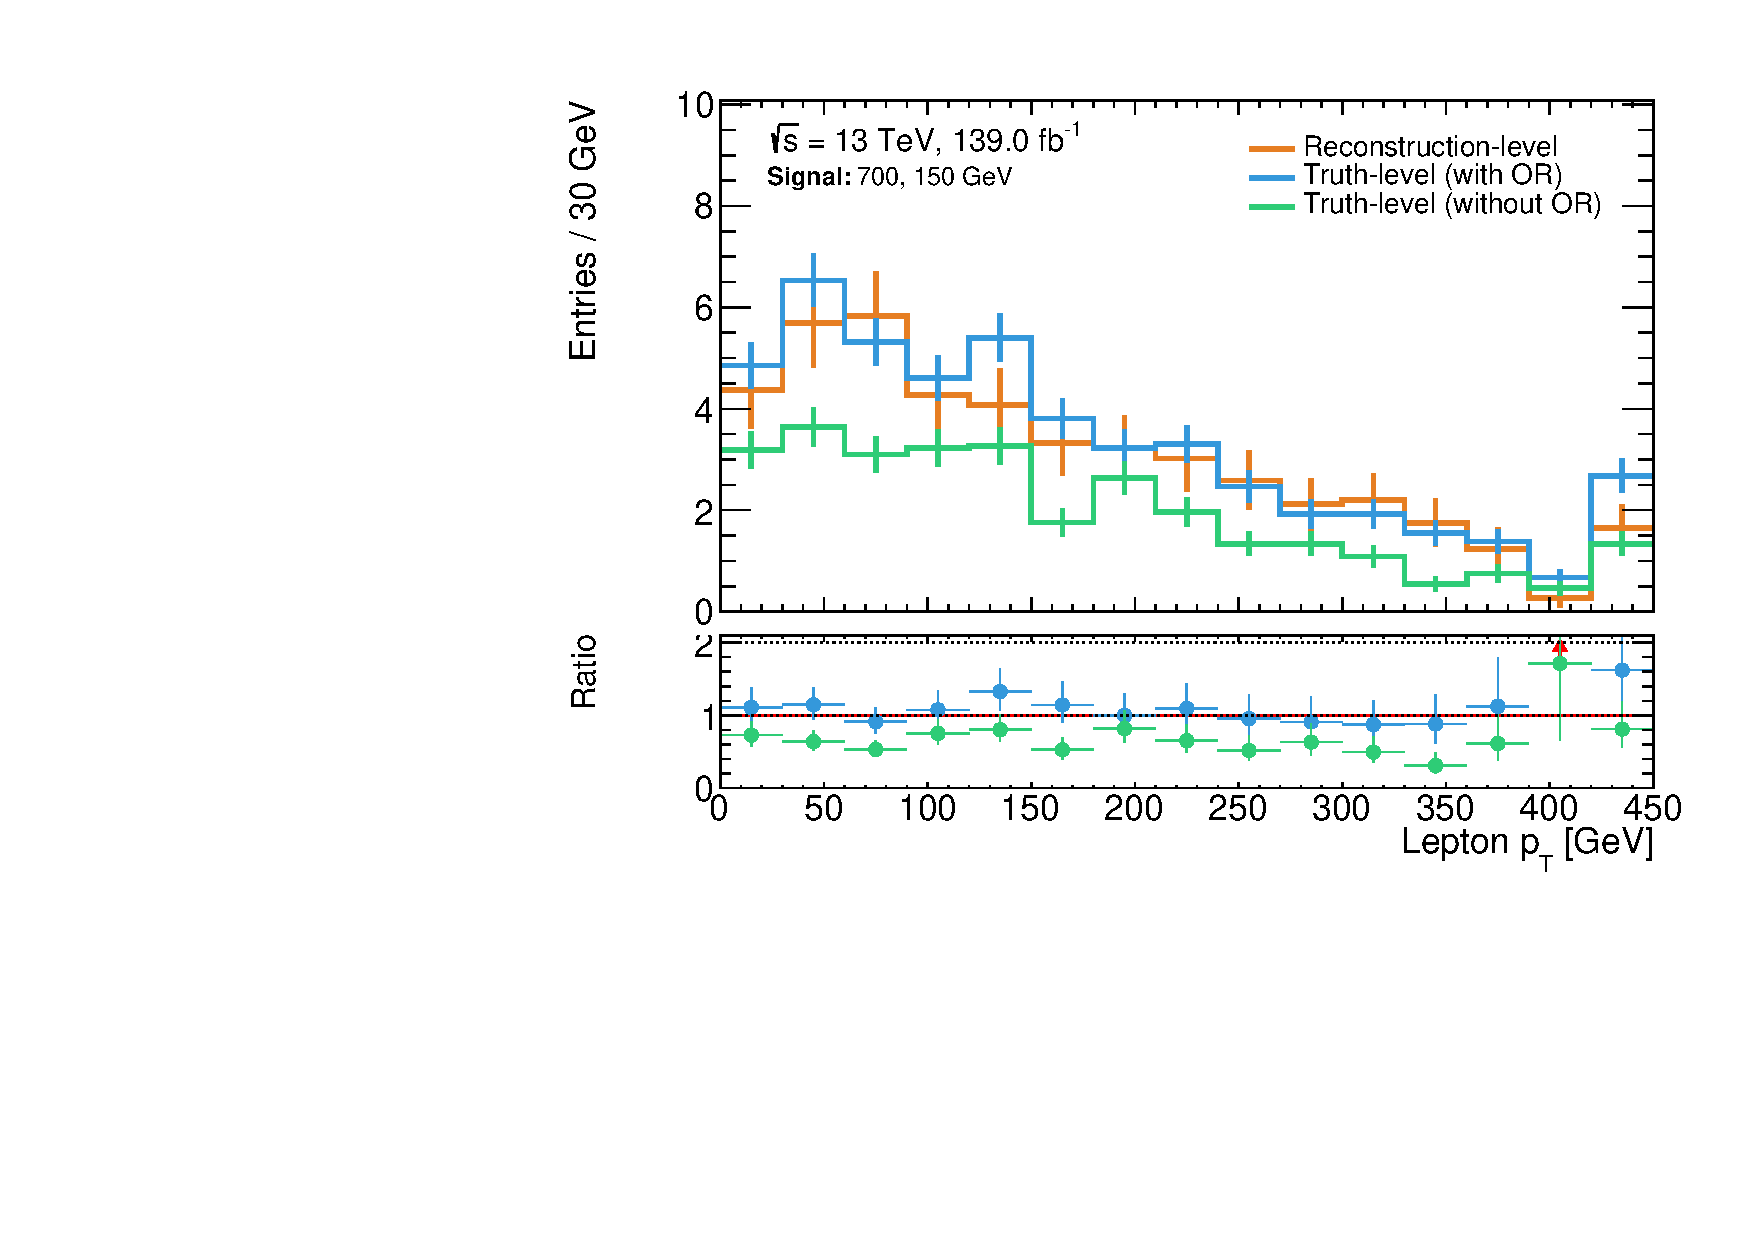
\includegraphics[width=\textwidth]{20210324_noLabel_noOR/700_150/lep1Pt_C1N2_Wh_hbb_700p0_150p0_smeared.pdf}
	\end{subfigure}\hfill
	\begin{subfigure}[b]{0.45\linewidth}
		\centering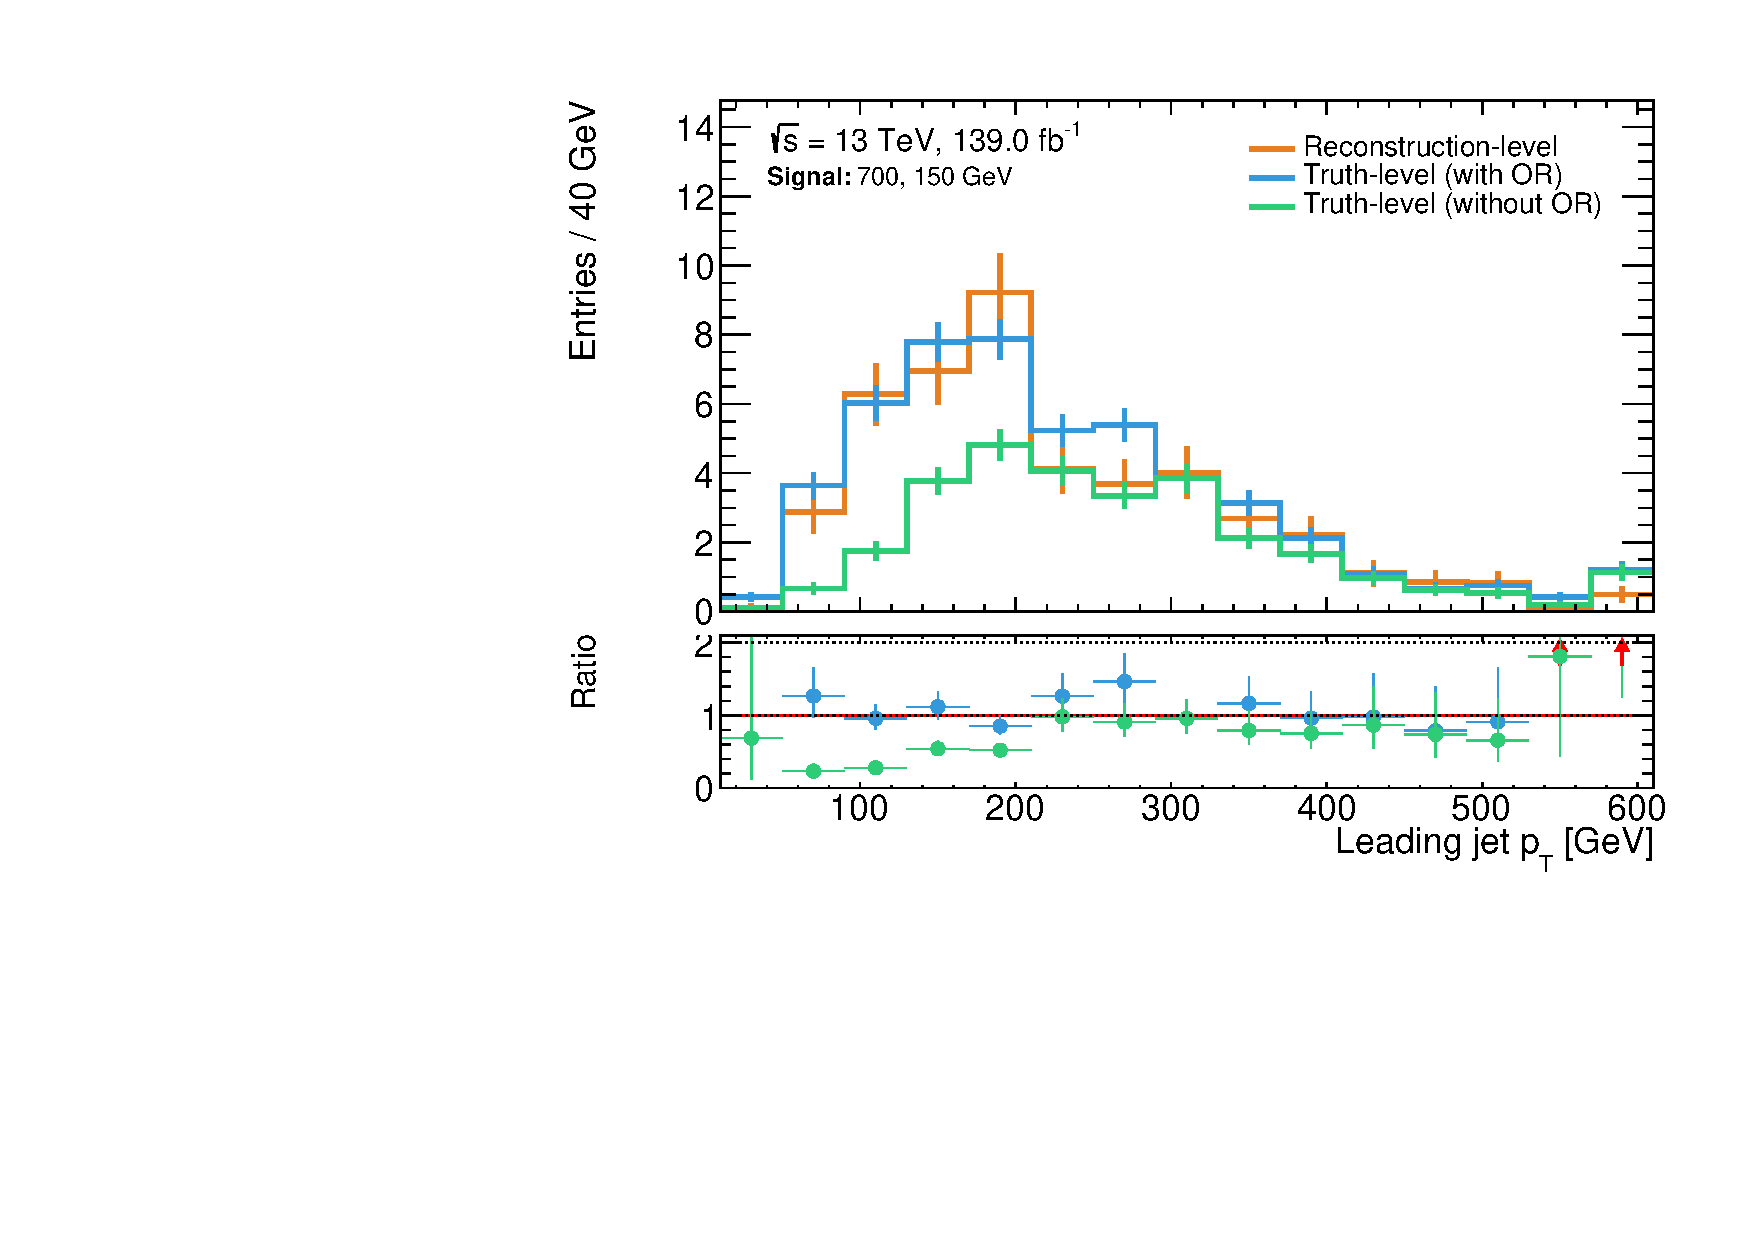
\includegraphics[width=\textwidth]{20210324_noLabel_noOR/700_150/jet1Pt_C1N2_Wh_hbb_700p0_150p0_smeared.pdf}
	\end{subfigure}\hfill
	\caption{Impact of the overlap removal procedure at truth-level illustrated in the lepton and leading jet transverse momenta distributions. The truth-distribution without overlap removal (green) generally underestimates the number of signal events at reconstruction-level (orange). Correct overlap removal procedure at truth-level (blue) improves the agreement. The exemplary benchmark signal point with $m(\charg/\neutr), m(\lsp) = 700, \SI{150}{\GeV}$ is shown in both plots (at truth- and reconstruction-level). All distributions are shown in a loose preselection requiring exactly one lepton, $\met>\SI{50}{\GeV}$, $\mt > \SI{50}{\GeV}$, and 2--3 jets, two of which need to be \textit{b}-tagged.}
	\label{fig:overlap_removal_truth}
\end{figure}

All signal and control regions considered in the original 1-lepton search are implemented at truth-level using \textsc{SimpleAnalysis}. The exact implementation is publicly available at \reference\cite{HEPdata_1Lbb} and was already used in~\cref{ch:uncertainties} for the derivation of some of the theory uncertainties in the full analysis.

The truth-level implementation full specifies all object definitions introduced in~\cref{sec:object_definitions} even though some of them, like \eg lepton isolation, are technically not well-defined at truth-level The subsequent smearing is in many cases implemented as a function of said object definitions and thus allows to consider them nonetheless. Additionally, as discussed in~\cref{sec:reinterpretations}, the full specification of the original analysis event selection including all object definitions allows for simpler reinterpretations by efforts outside of the ATLAS collaboration that generally do not have access to the original analysis software.

Following the object definitions, an overlap removal procedure following the same prescription as described for the reconstruction-level analysis is performed, \ie especially also using the same shrinking cone definitions introduced in~\cref{sec:overlap_removal}. Overlap removal step removing electrons sharing a track with a muon is approximated by using a distance parameter of $\Delta R = 0.01$ between the objects. Although often neglected\footnote{The overlap removal procedures in ATLAS \gls{susy} searches tend to be quite intricate, making them non-trivial to re-implement without ATLAS and analysis-specific knowledge.} in reinterpretation efforts outside of the collaboration, the correct implementation of the overlap removal procedure employed in the original analysis is typically crucial to reproduce the signal estimates of the original analysis, as illustrated in~\cref{fig:overlap_removal_truth}. Furthermore, the exact implementation of all analysis observables is explicitly given in the \textsc{SimpleAnalysis} implementation, followed by the full definition of all control and signal regions.

\subsection{Truth smearing}\label{sec:truth_smearing}

The general assumption of the truth smearing applied in the following is that the detector response roughly factorises into the responses of single particles. This allows to use detector performance results provided by ATLAS in order to construct detector response maps parameterised in different observables for each physics object. Detector response maps include object reconstruction and identification efficiencies as well as scale factors to correct for differences between \gls{mc} and observed data. Likewise, effects from the finite resolution of energy measurements in the detector are modelled through energy resolution maps. In the following, the 4-vector components of electrons, muons, jets and $\etmiss$ are smeared. The implementation of the smearing functions is internal to ATLAS and originates predominantly from various upgrade studies.

In the case of truth electrons, the identifications efficiencies considered are parameterised in $\eta$ and $\pt$ as well as the identification working point used. In $\eta$, nine fixed-width bins are used. In $\pt$, six bins are implemented and a linear interpolation between two adjacent $\pt$-bins is used to get the efficiency for the given $\pt$ of each truth electron. The probability of finding a fake electron in a truth jet is estimated through a similar two-dimensional map depending on the truth jet $\eta$ and $\pt$, again using fixed-width bins in $\eta$ and a linear interpolation in $\pt$. The range of the $\pt$ interpolation for identification efficiencies and fake rates extends from $\SI{7}{\GeV}$ to $\SI{120}{\GeV}$. If the truth $\pt$ of the electron is outside of that range, the identification efficiency and fake rate from the respective bound of the corresponding $\eta$-bin are used. The probability for misidentifying an electron as a photon is estimated using different fixed values for the barrel and end-cap regions. Finally, the transverse energy of the electron is smeared using a random number drawn from a Gaussian distribution with  standard deviation corresponding to the $\eta$- and $\pt$-dependent energy resolution.  

For truth muons, the identification efficiencies are also parameterised in $\eta$ and $\pt$ as well as the identification working point used. Similar to truth electrons, the  $\pt$ of the muon is smeared using a Gaussian distribution with standard deviation corresponding to the momentum resolution. The momentum resolution of combined truth muons, $\sigma_\mathrm{CB}$, is computed from the measured resolutions in the \gls{id},$\sigma_\mathrm{ID}$, and \gls{ms}, $\sigma_\mathrm{MS}$, as
\begin{equation}
	\sigma_\mathrm{CB} = \frac{\sigma_\mathrm{ID}\sigma_\mathrm{MS}}{\sqrt{\sigma_\mathrm{ID}^2 + \sigma_\mathrm{MS}^2}},
\end{equation}
where $\sigma_\mathrm{ID}$ and $\sigma_\mathrm{MS}$ are parameterised in $\eta$ and $\pt$.

The transverse momentum of truth jets is smeared using a Gaussian with standard deviation equal to the \gls{jer}, provided in a map parameterised in five bins in $\eta$ ranging from $\vert\eta\vert = 0$ to $\vert\eta\vert = 4.5$. Following~\cite{Aad:2020flx}, jet energy resolutions are provided using parameterisations of a noise $N$, stochastic $S$ and constant $C$ term for each of the seven bins in $\vert\eta\vert$, such that the resolution can be computed as
\begin{equation}
	\frac{\sigma(\pt)}{\pt} = \frac{N}{\pt}\oplus\frac{S}{\sqrt{\pt}}\oplus C.
\end{equation}
Only truth jets with $\SI{10}{\GeV} < \pt < \SI{1.5}{\TeV}$ are smeared. For truth jets with $\pt > \SI{20}{\GeV}$, the flavour tagging efficiency is considered using efficiencies parameterised in $\eta$, $\pt$ and the \textsc{MV2c10} working point (introduced in~\cref{sec:object_definitions}) used, measured in fully reconstructed simulated $\ttbar$ events~\cite{FTAG-2018-01}.

Finally, the smeared missing transverse energy is computed using the transverse momenta of all smeared truth objects in the event, including an approximation for the track soft term. The latter is approximated using results from $Z\rightarrow e^+e^-$ events, allowing to infer a distribution of the mean soft term projected in the direction longitudinal to the total transverse momentum of all hard objects in an event, $\boldsymbol{p}_\mathrm{T}^\mathrm{hard}$. The measured resolution parallel and perpendicular to $\boldsymbol{p}_\mathrm{T}^\mathrm{hard}$ is then used to smear the nominal soft track value.
 
  \begin{figure}
	\centering
	\begin{subfigure}[b]{0.45\linewidth}
		\centering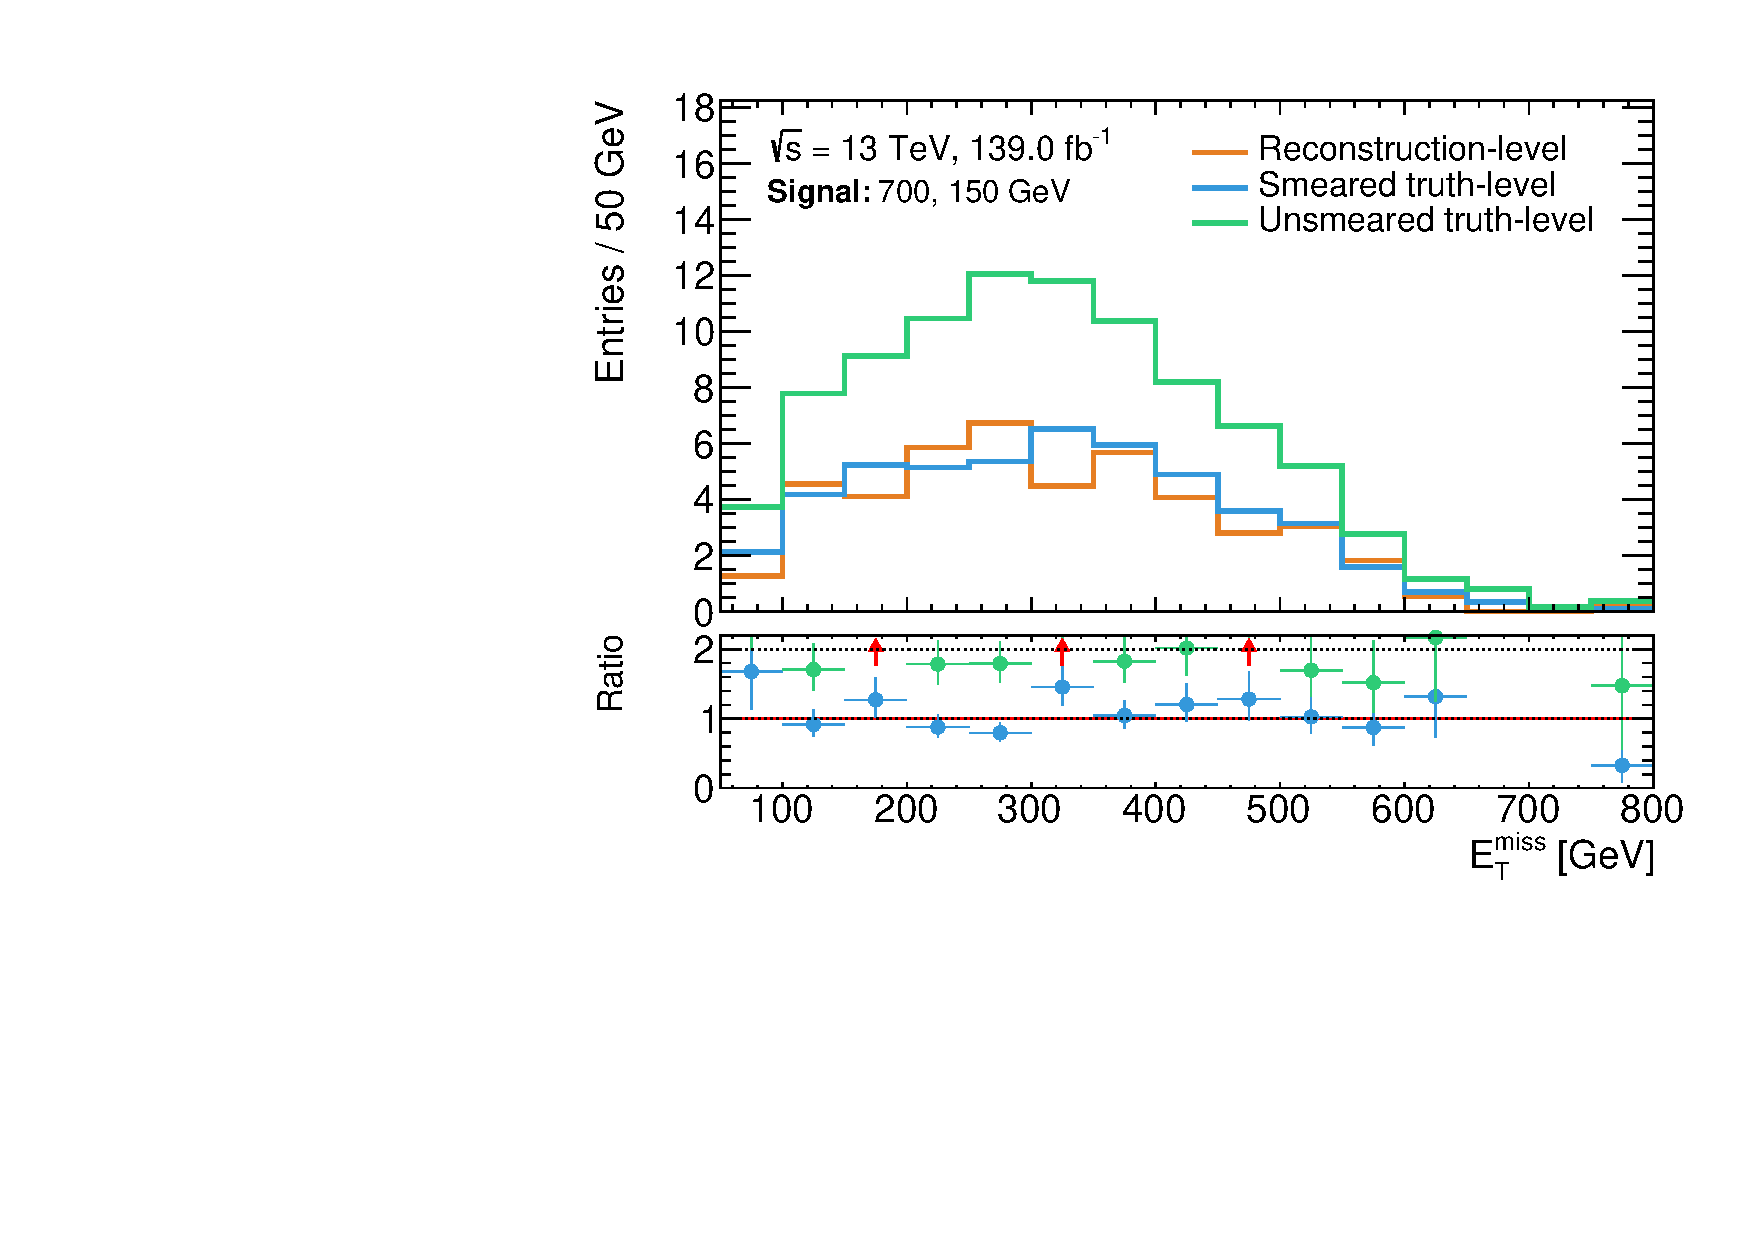
\includegraphics[width=\textwidth]{20210324/700_150/met_C1N2_Wh_hbb_700p0_150p0_smeared.pdf}
	\end{subfigure}\hfill
	\begin{subfigure}[b]{0.45\linewidth}
		\centering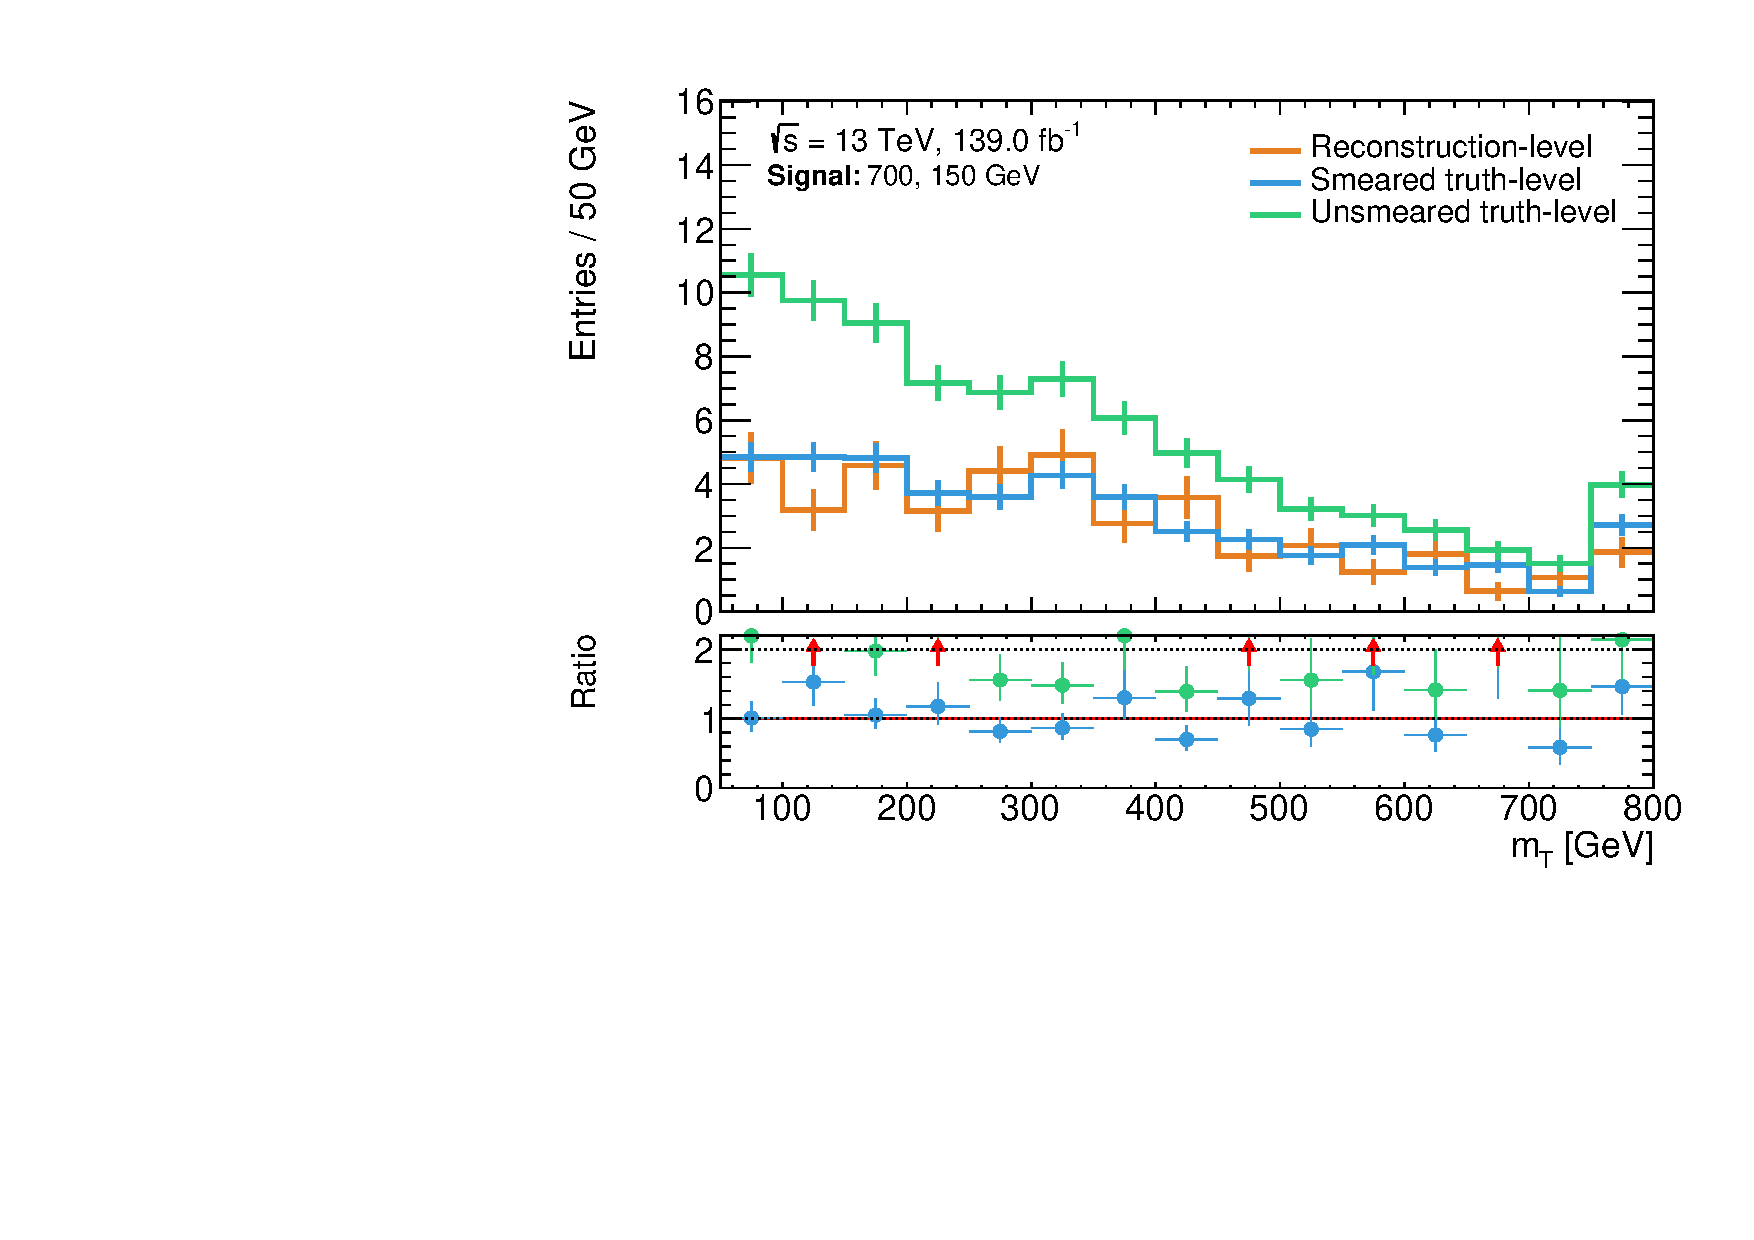
\includegraphics[width=\textwidth]{20210324/700_150/mt_C1N2_Wh_hbb_700p0_150p0_smeared.pdf}
	\end{subfigure}\hfill
	\begin{subfigure}[b]{0.45\linewidth}
		\centering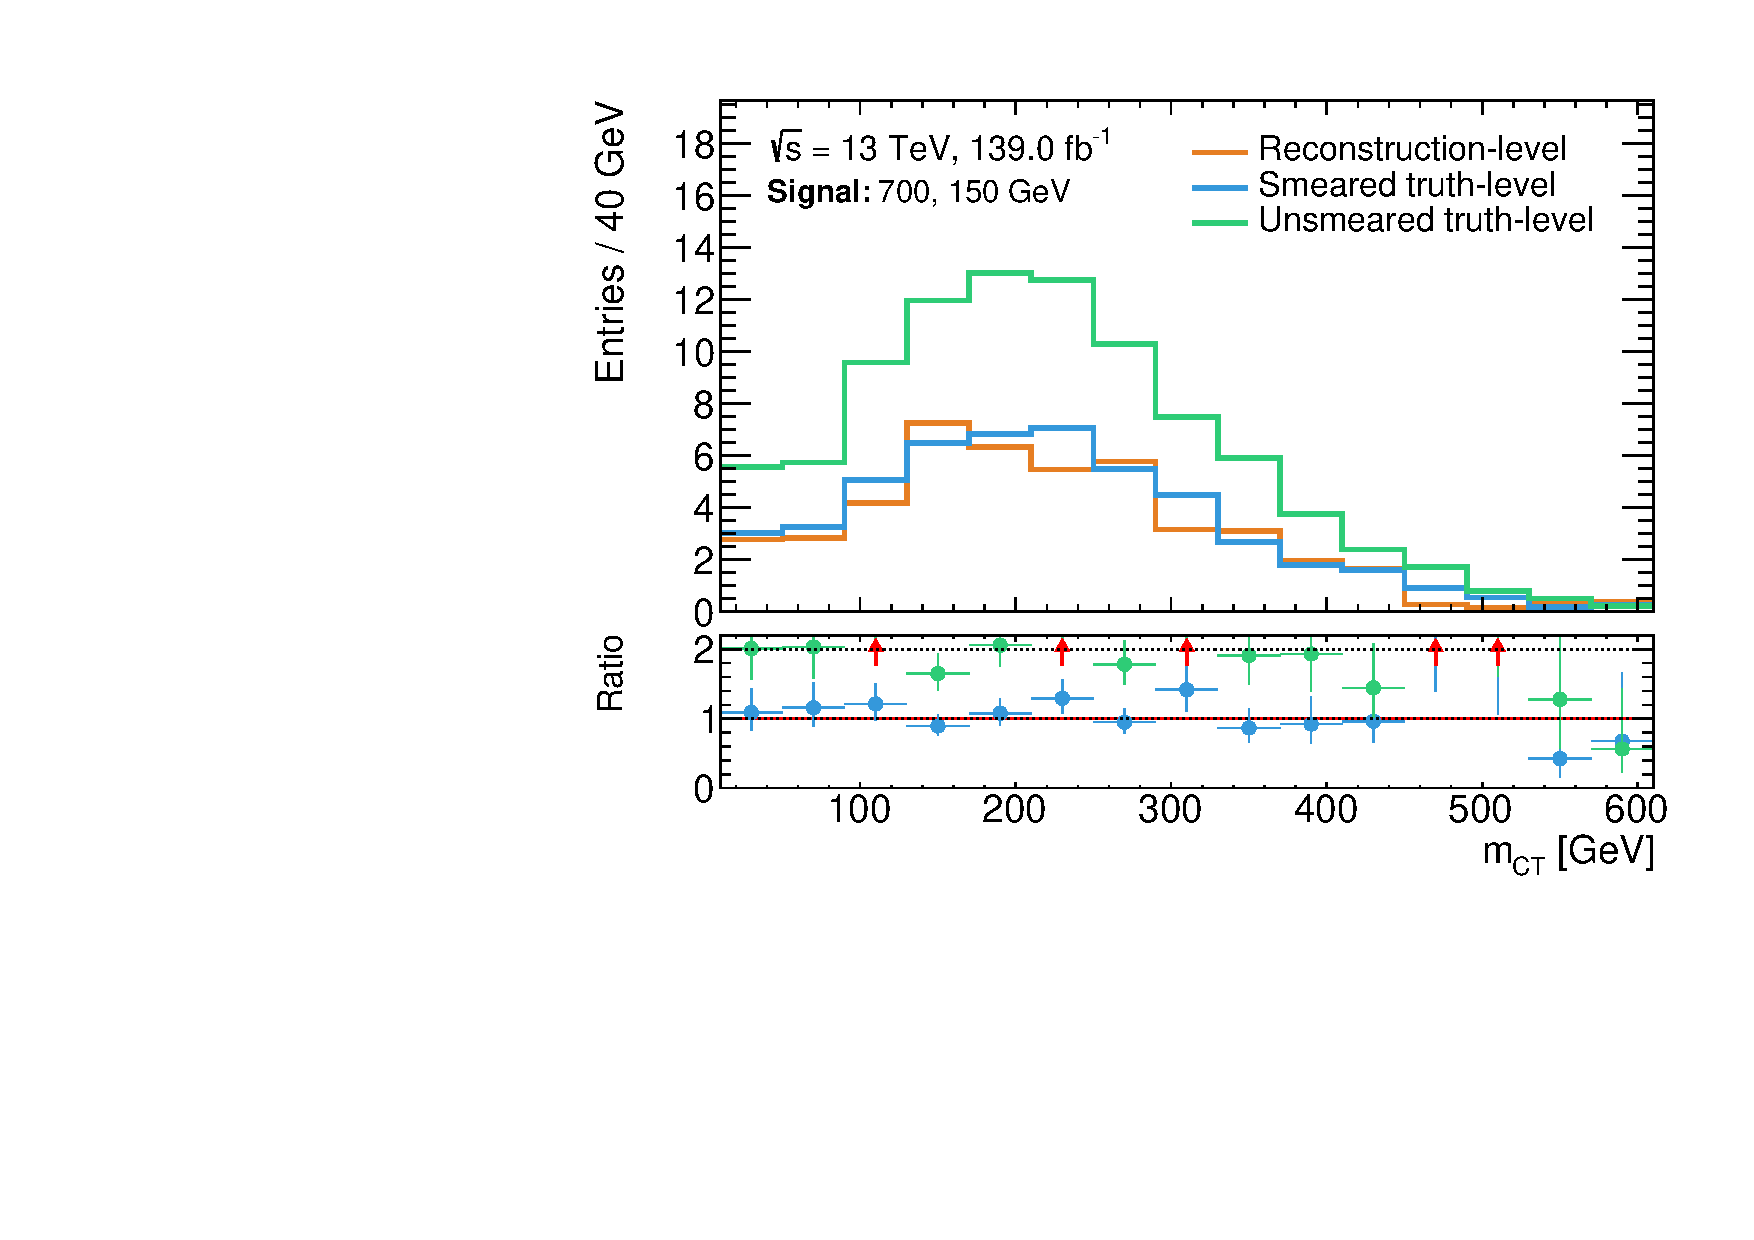
\includegraphics[width=\textwidth]{20210324/700_150/mct_C1N2_Wh_hbb_700p0_150p0_smeared.pdf}
	\end{subfigure}\hfill
	\begin{subfigure}[b]{0.45\linewidth}
		\centering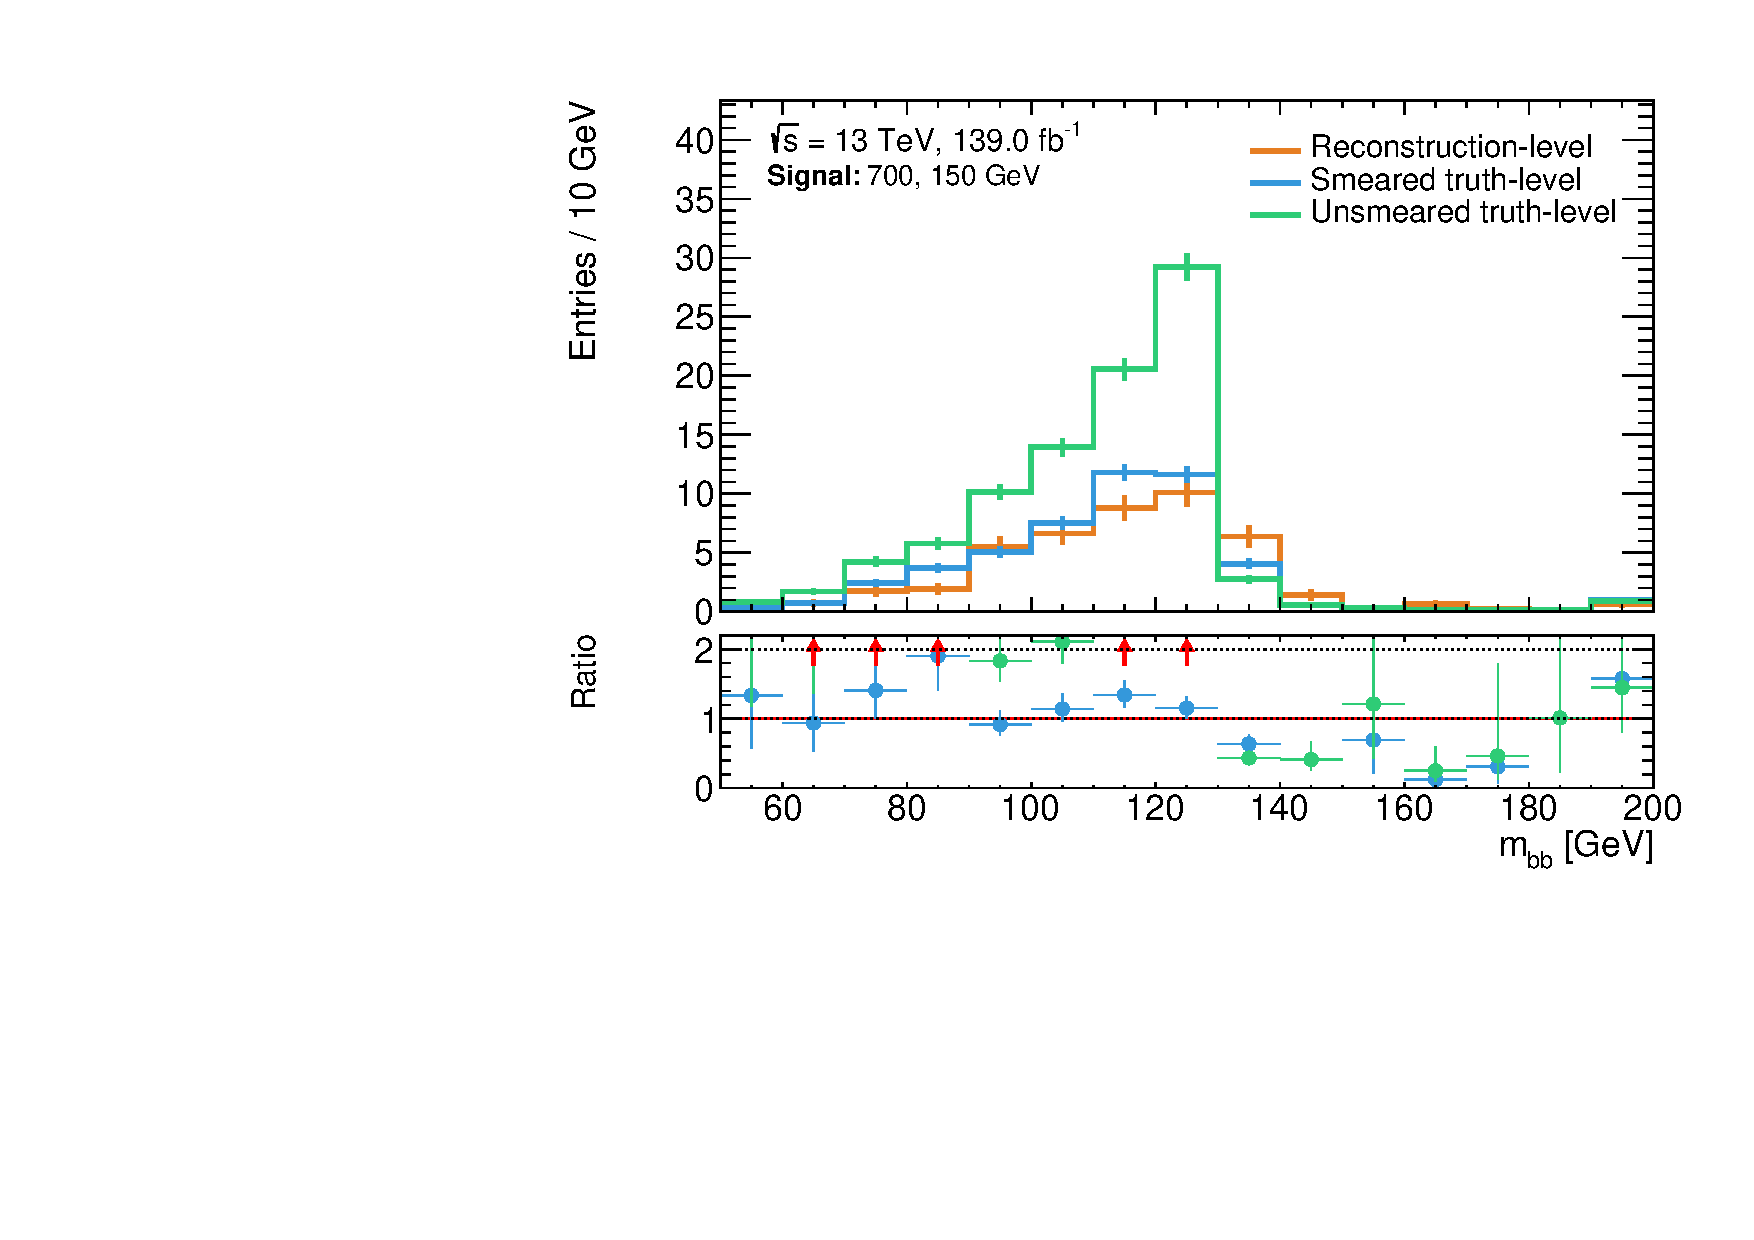
\includegraphics[width=\textwidth]{20210324/700_150/mbb_C1N2_Wh_hbb_700p0_150p0_smeared.pdf}
	\end{subfigure}\hfill
	\begin{subfigure}[b]{0.45\linewidth}
		\centering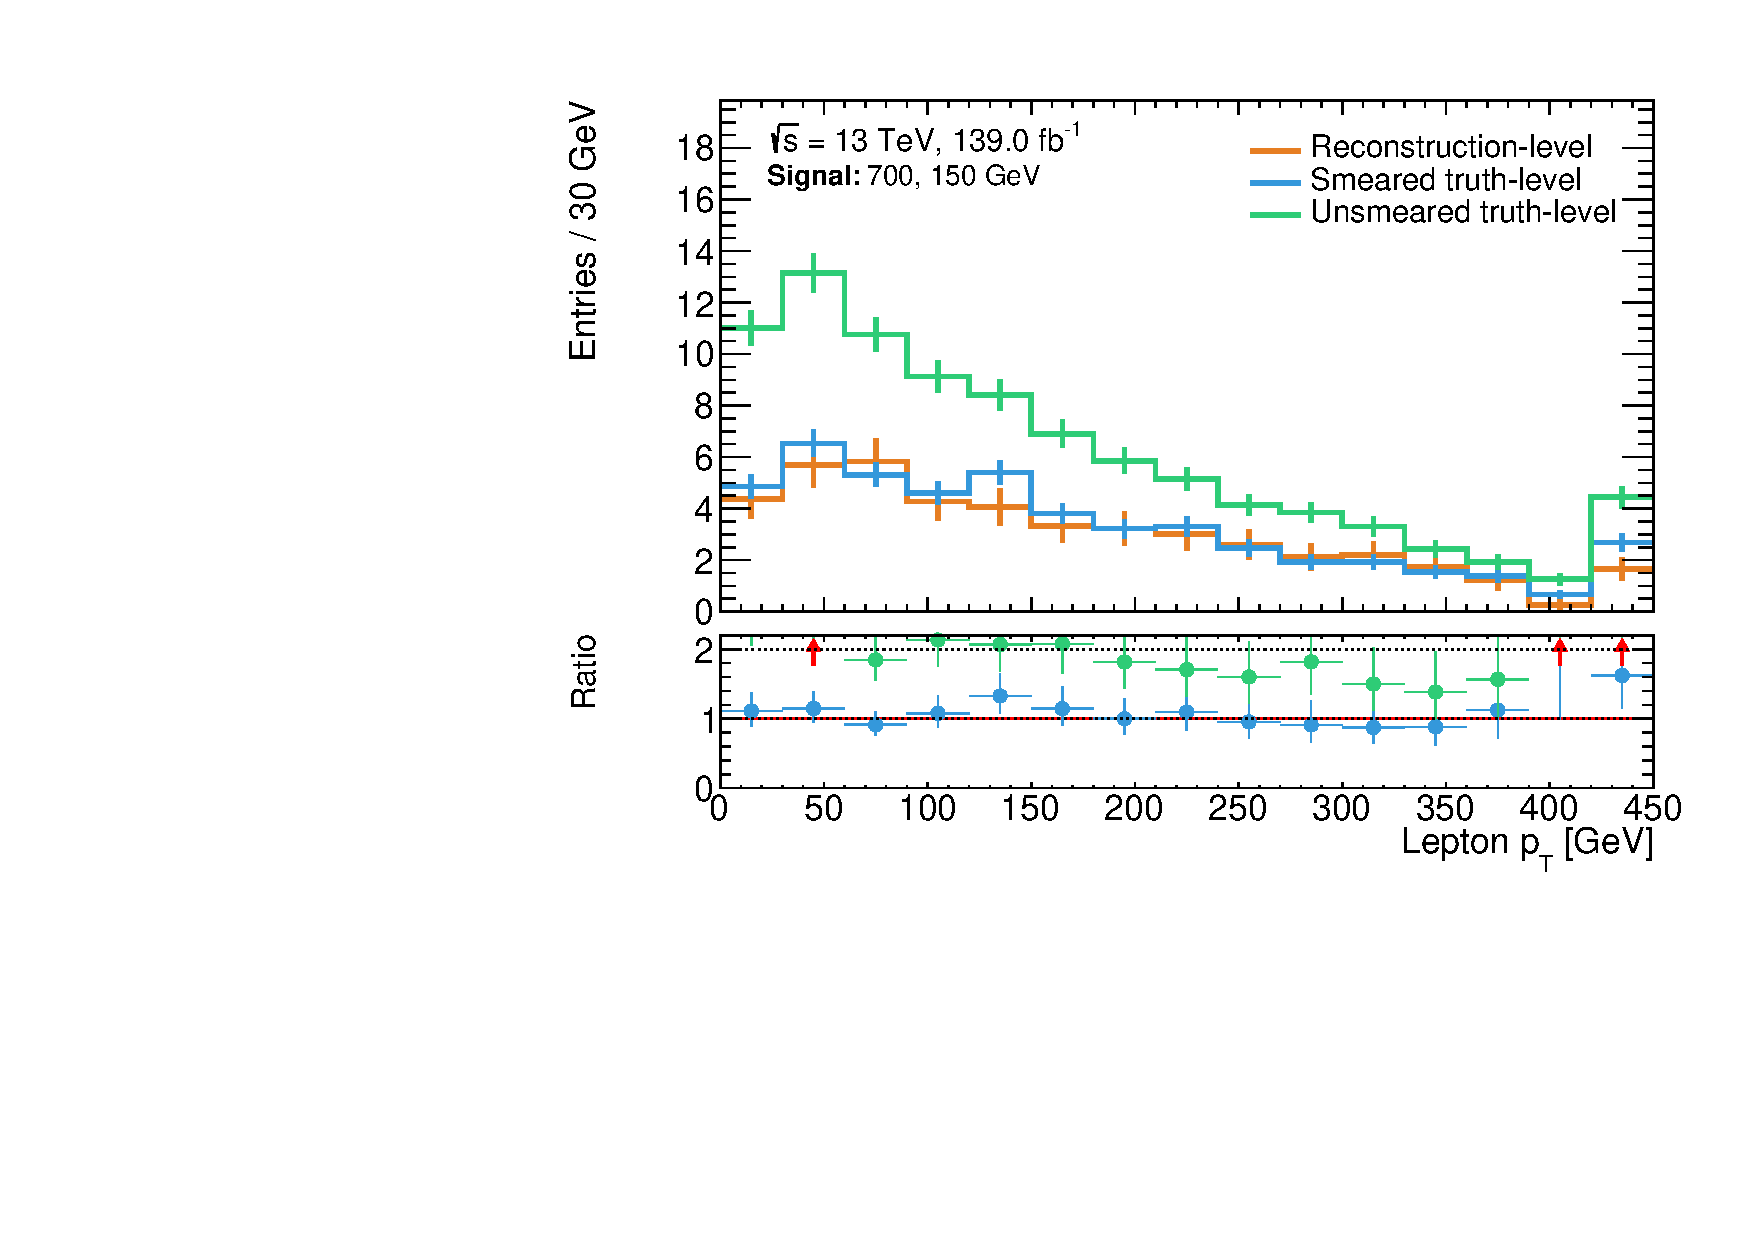
\includegraphics[width=\textwidth]{20210324/700_150/lep1Pt_C1N2_Wh_hbb_700p0_150p0_smeared.pdf}
	\end{subfigure}\hfill
	\begin{subfigure}[b]{0.45\linewidth}
		\centering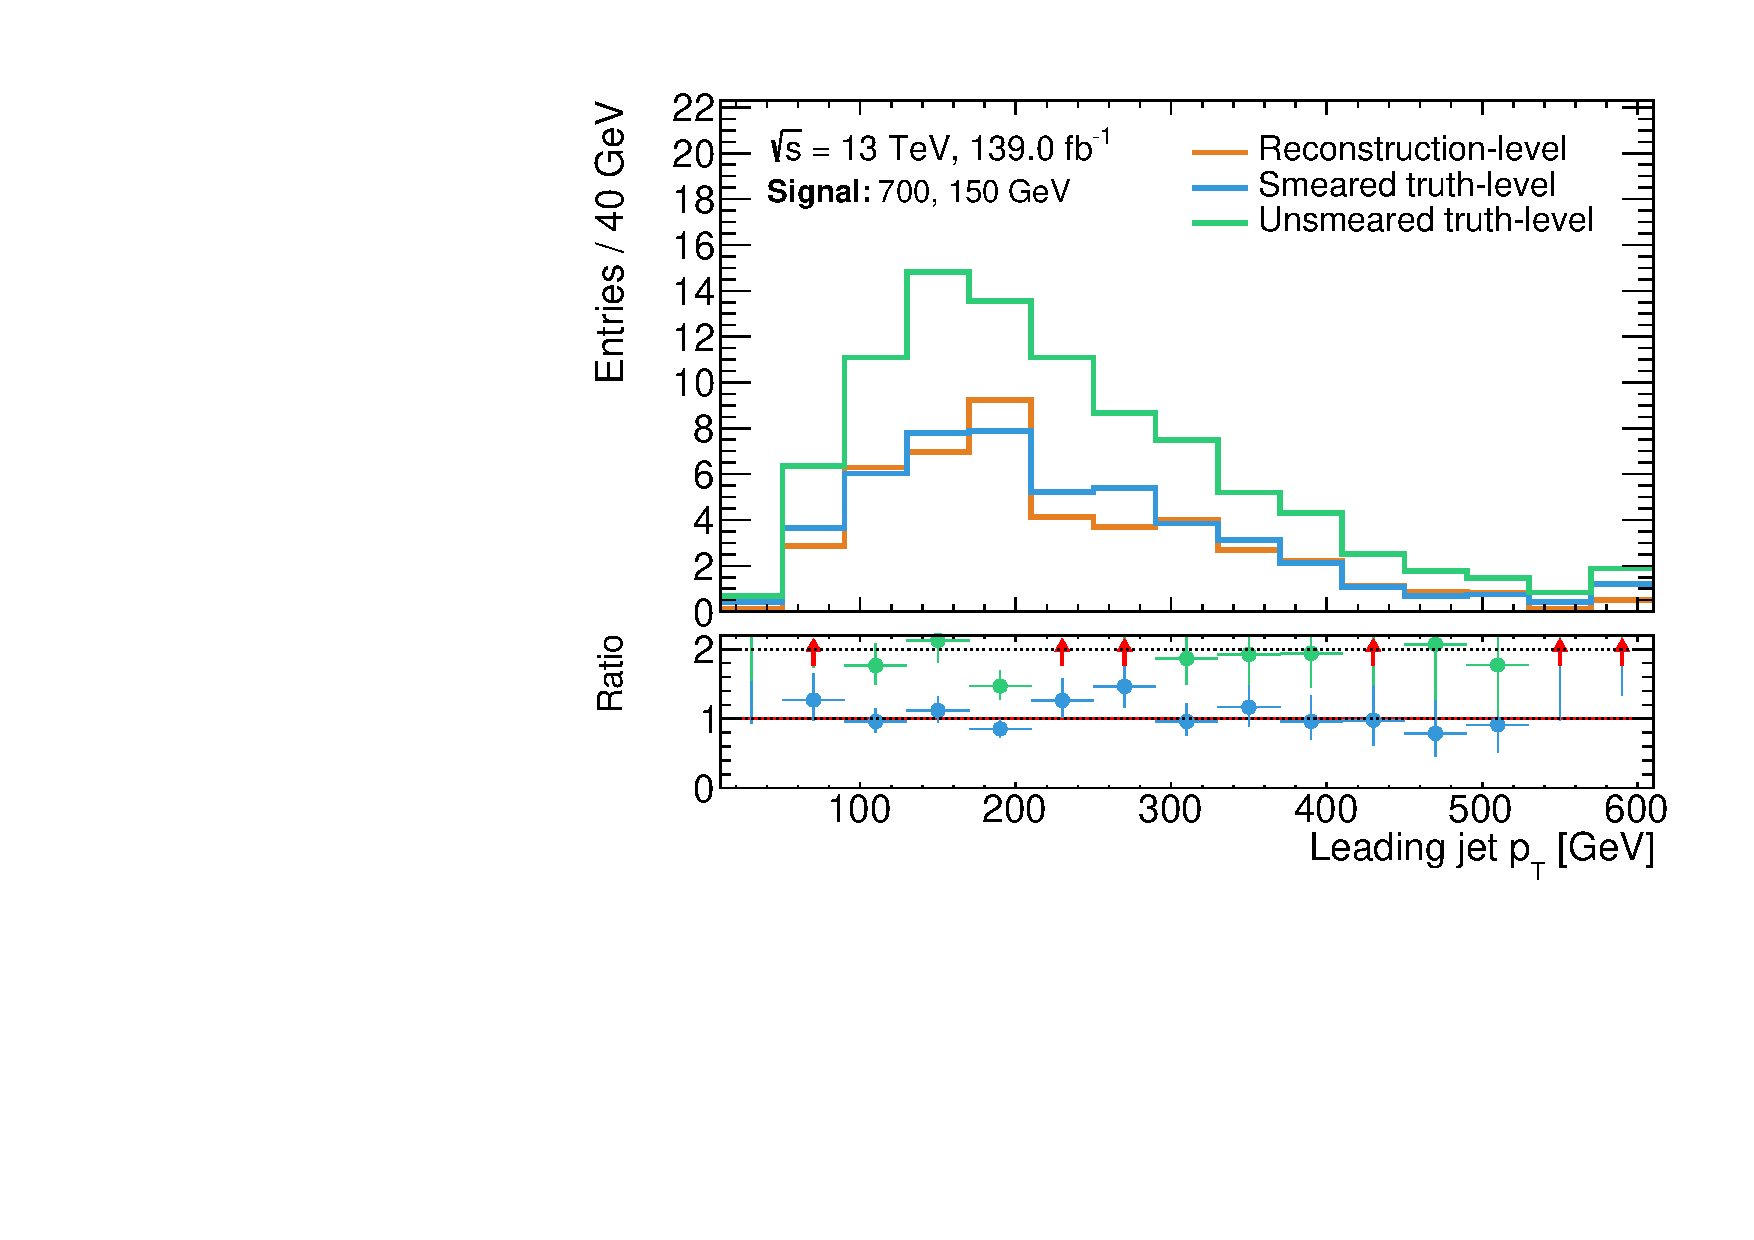
\includegraphics[width=\textwidth]{20210324/700_150/jet1Pt_C1N2_Wh_hbb_700p0_150p0_smeared.pdf}
	\end{subfigure}\hfill
	\begin{subfigure}[b]{0.45\linewidth}
		\centering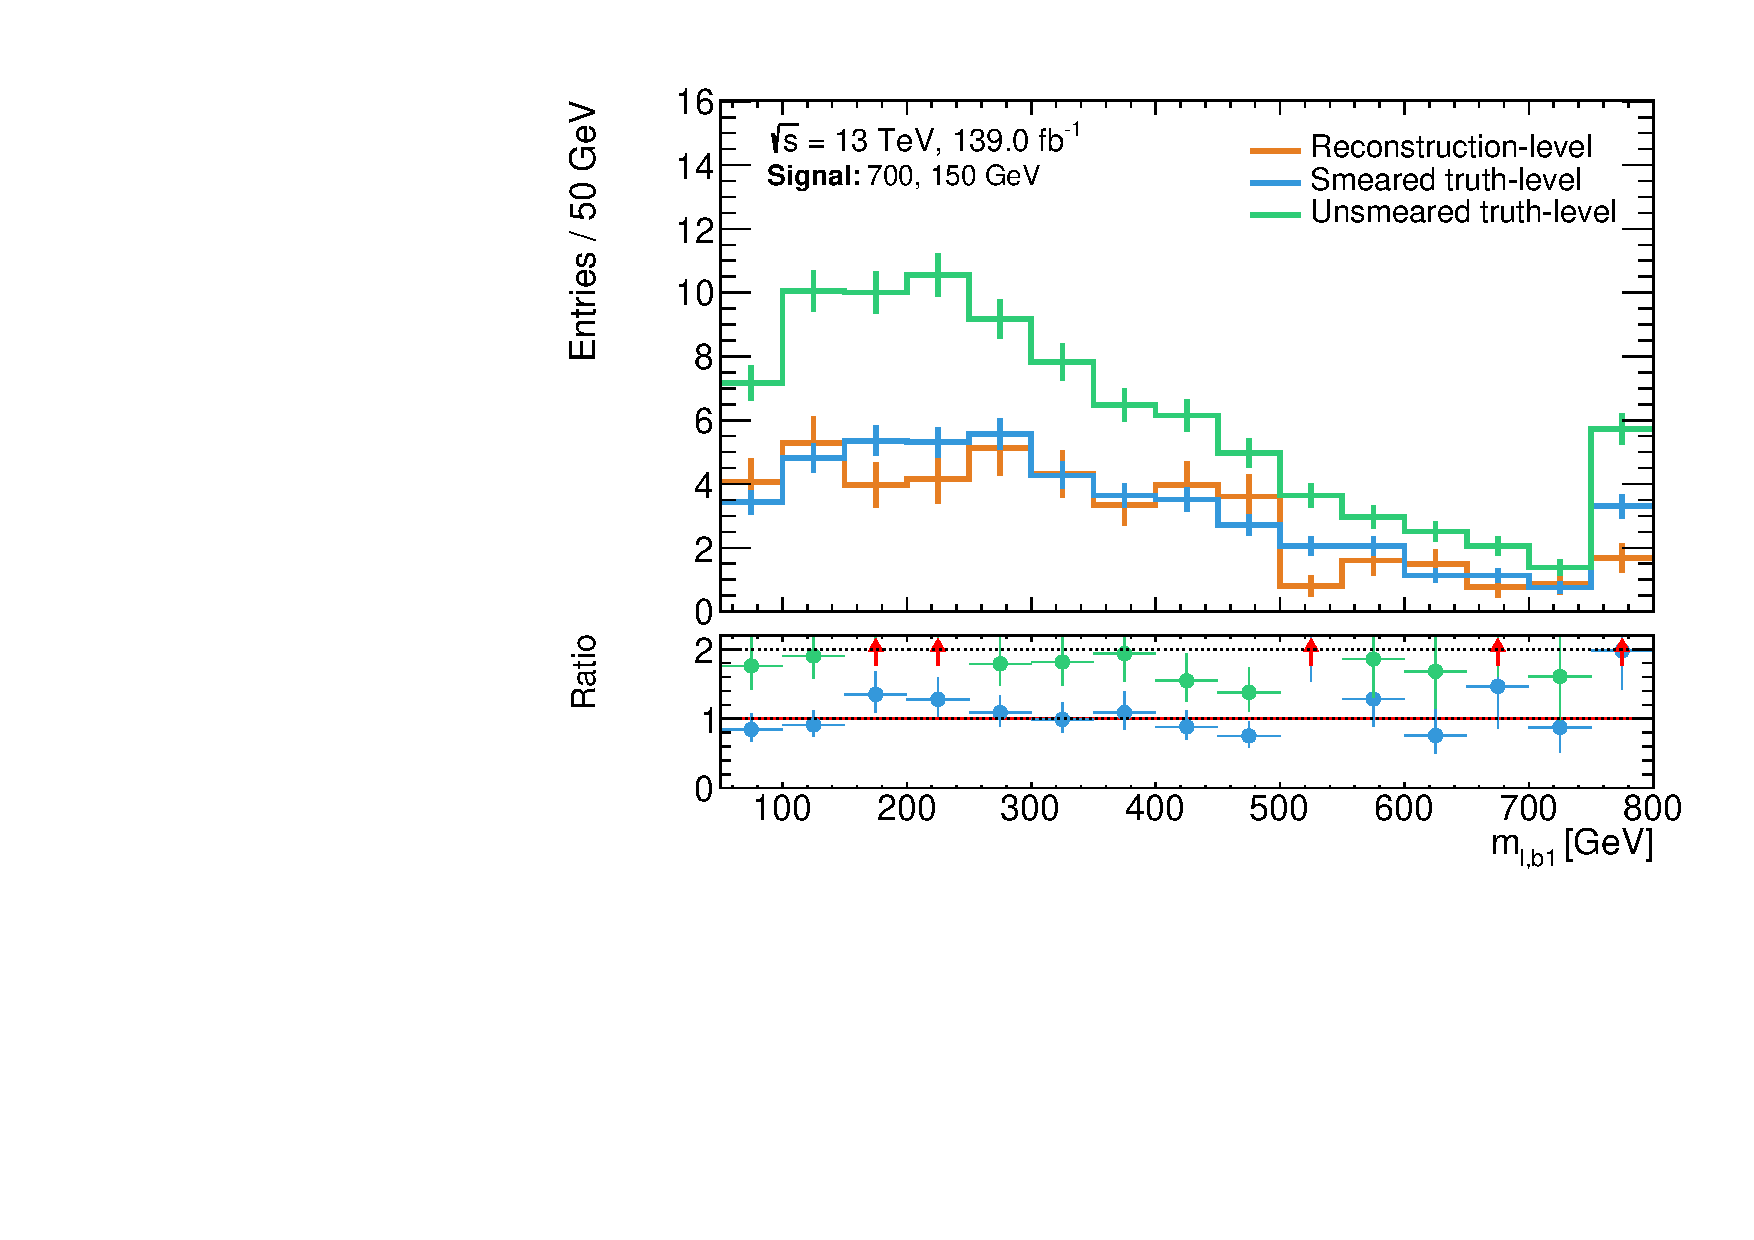
\includegraphics[width=\textwidth]{20210324/700_150/mlb1_C1N2_Wh_hbb_700p0_150p0_smeared.pdf}
	\end{subfigure}\hfill
	\begin{subfigure}[b]{0.45\linewidth}
		\centering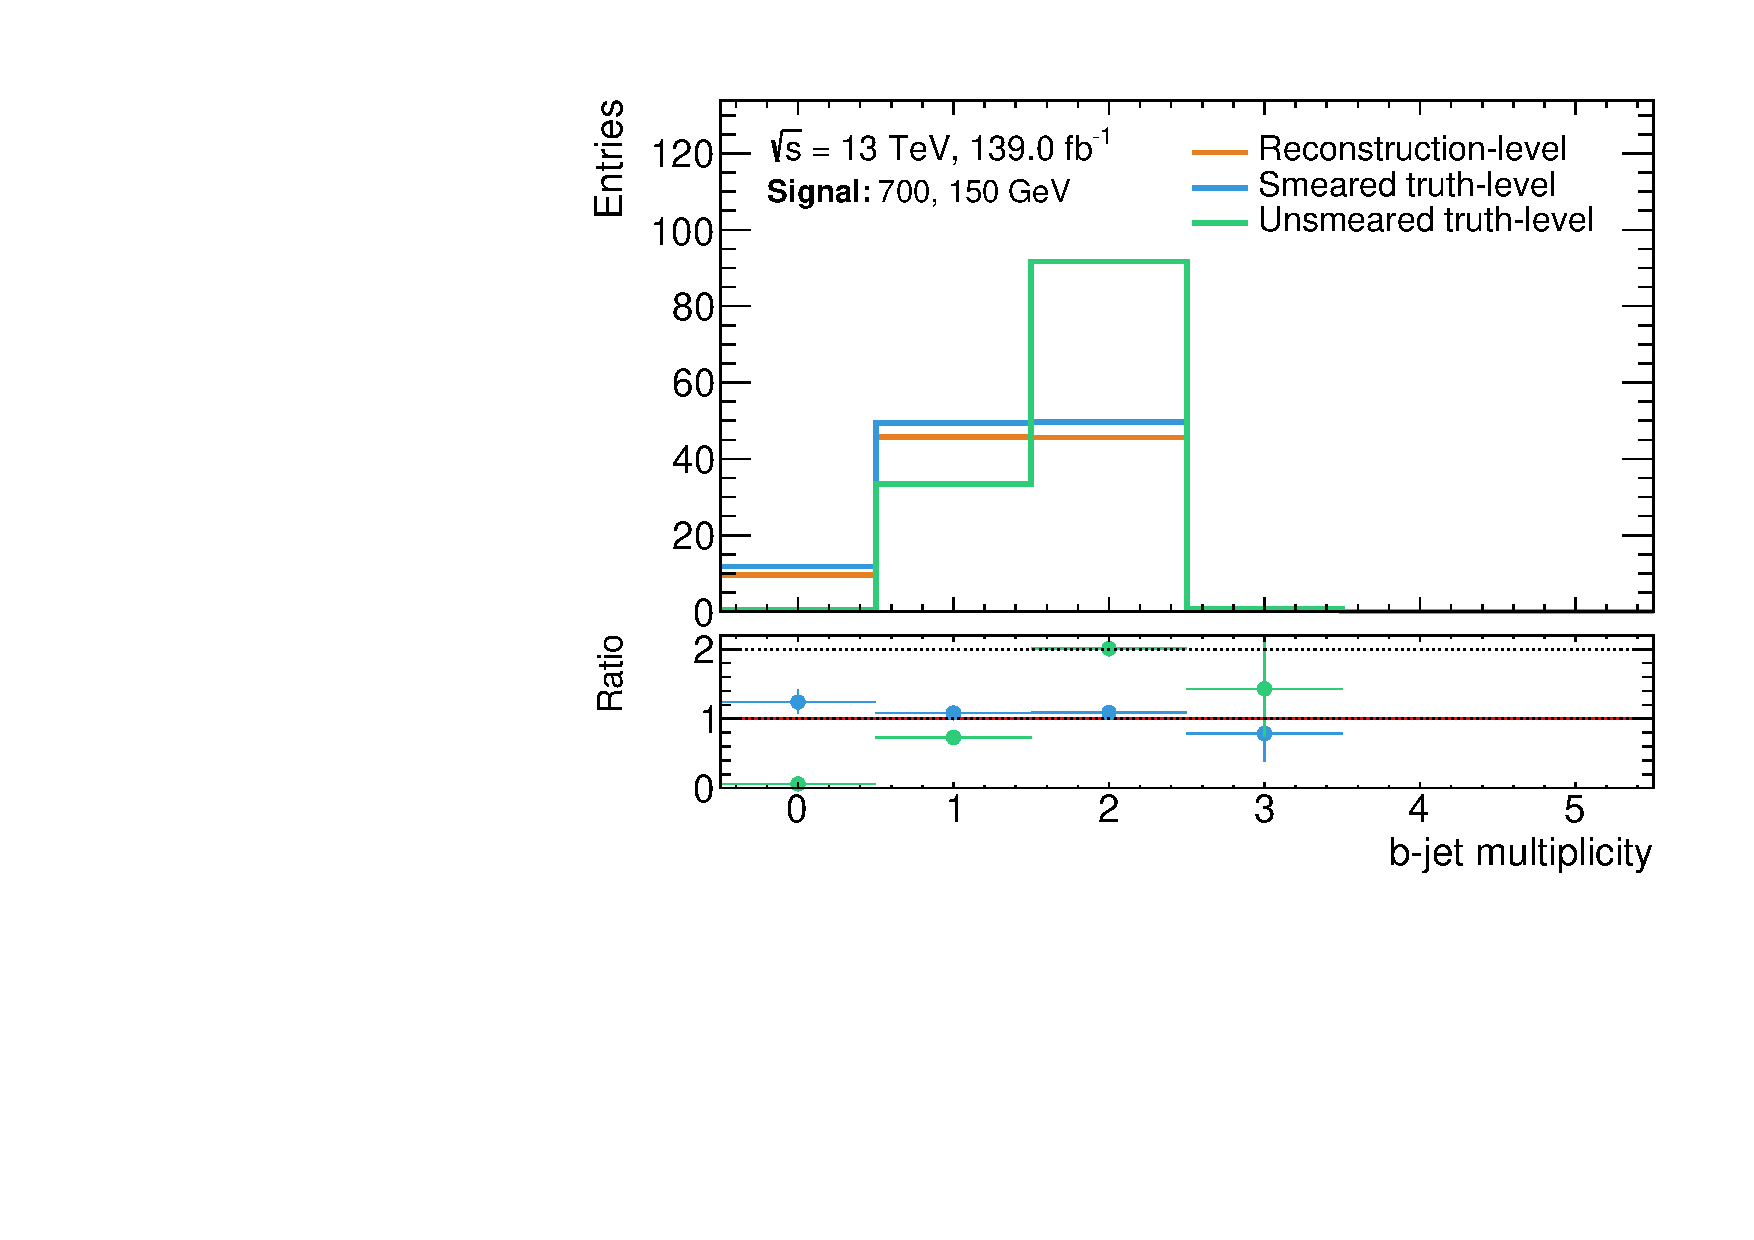
\includegraphics[width=\textwidth]{20210324/700_150/nBJet30_C1N2_Wh_hbb_700p0_150p0_smeared.pdf}
	\end{subfigure}\hfill
	\caption{Comparisons of the kinematic distributions of key observables at (smeared) truth- and reconstruction-level. The exemplary benchmark signal point with $m(\charg/\neutr), m(\lsp) = 700, \SI{150}{\GeV}$ is shown. The ratio pad shows the ratio between smeared and unsmeared truth-level distributions (blue and green) to reconstruction-level distributions (orange). Only \gls{mc} statistical uncertainty is included in the error bars. All distributions are shown in a loose preselection requiring exactly one lepton, $\met>\SI{50}{\GeV}$, $\mt > \SI{50}{\GeV}$, and 2--3 jets, two of which need to be \textit{b}-tagged. The latter requirement is dropped for the \textit{b}-jet multiplicity distribution.}
	\label{fig:smearing_preselection}
\end{figure}
 
\section{Validation of the truth-level analysis}

\subsection{Validation in loose preselection}

 The performance of the truth smearing is illustrated in a loose preselection for a single exemplary benchmark signal point in~\cref{fig:smearing_preselection}. The loose preselection applied requires exactly one lepton, $\met>\SI{50}{\GeV}$, $\mt > \SI{50}{\GeV}$, and 2--3 jets, two of which need to be \textit{b}-tagged. The reconstruction-level distributions are compared with the truth-level distributions before and after truth smearing. It can clearly be observed that the truth smearing noticeably improves the agreement between the truth- and reconstruction-level distributions. While the lepton and jet reconstruction and identification efficiencies are---due to their dependence on $\eta$, $\pt$ and individual working points---crucial for the overall agreement in shape, the inclusion of flavour-tagging efficiencies significantly improves the overall agreement in normalisation.
 
Although some minor differences remain, overall a good agreement is observed across all relevant kinematic distributions at loose preselection level. Most of the differences between smeared truth-level and reconstruction-level distributions in individual bins are well within the \gls{mc} statistical uncertainties arising from the relatively limited \gls{mc} statistics available.
 
 \subsection{Validation in signal regions}

 \begin{figure}
	\centering
	\begin{subfigure}[b]{0.49\linewidth}
		\centering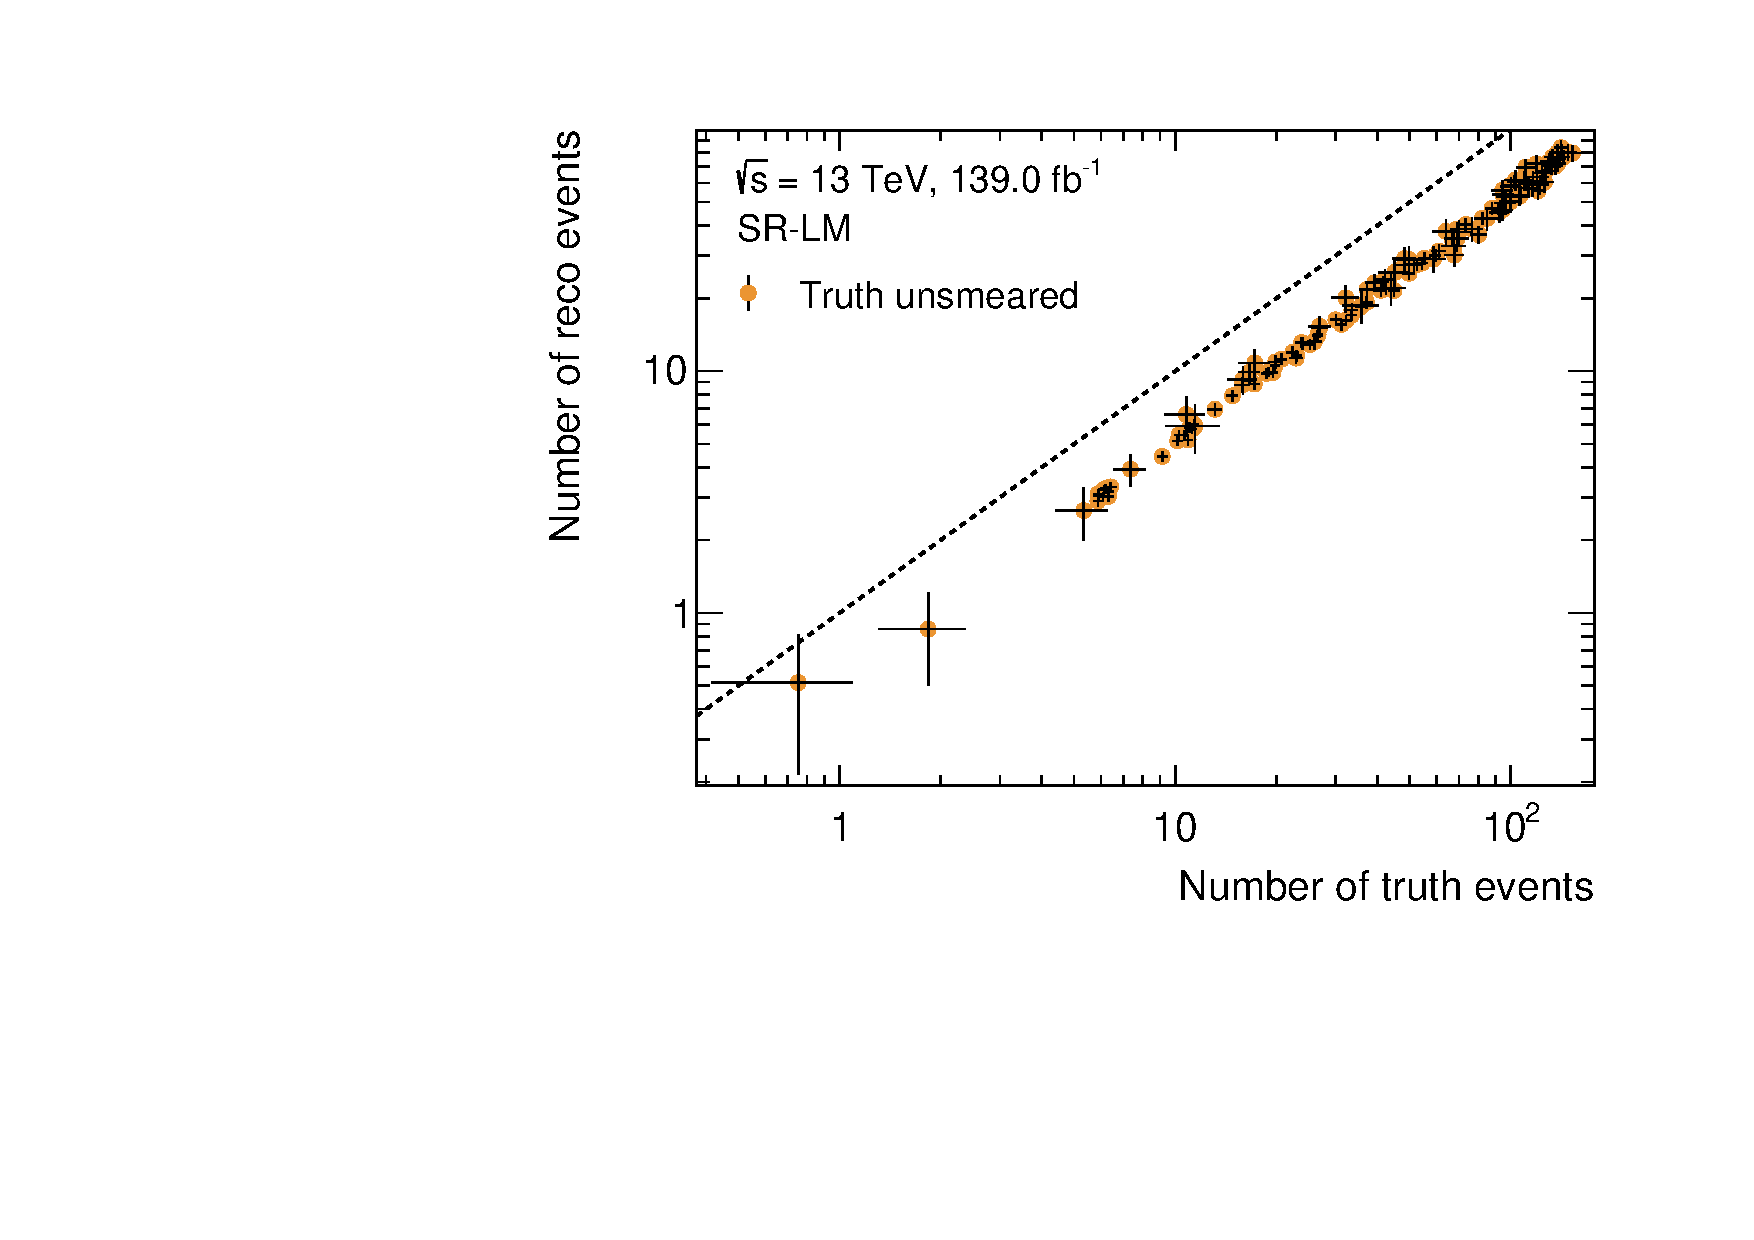
\includegraphics[width=\textwidth]{yields_SR-LM_unsmeared}
	\end{subfigure}\hfill
	\begin{subfigure}[b]{0.49\linewidth}
		\centering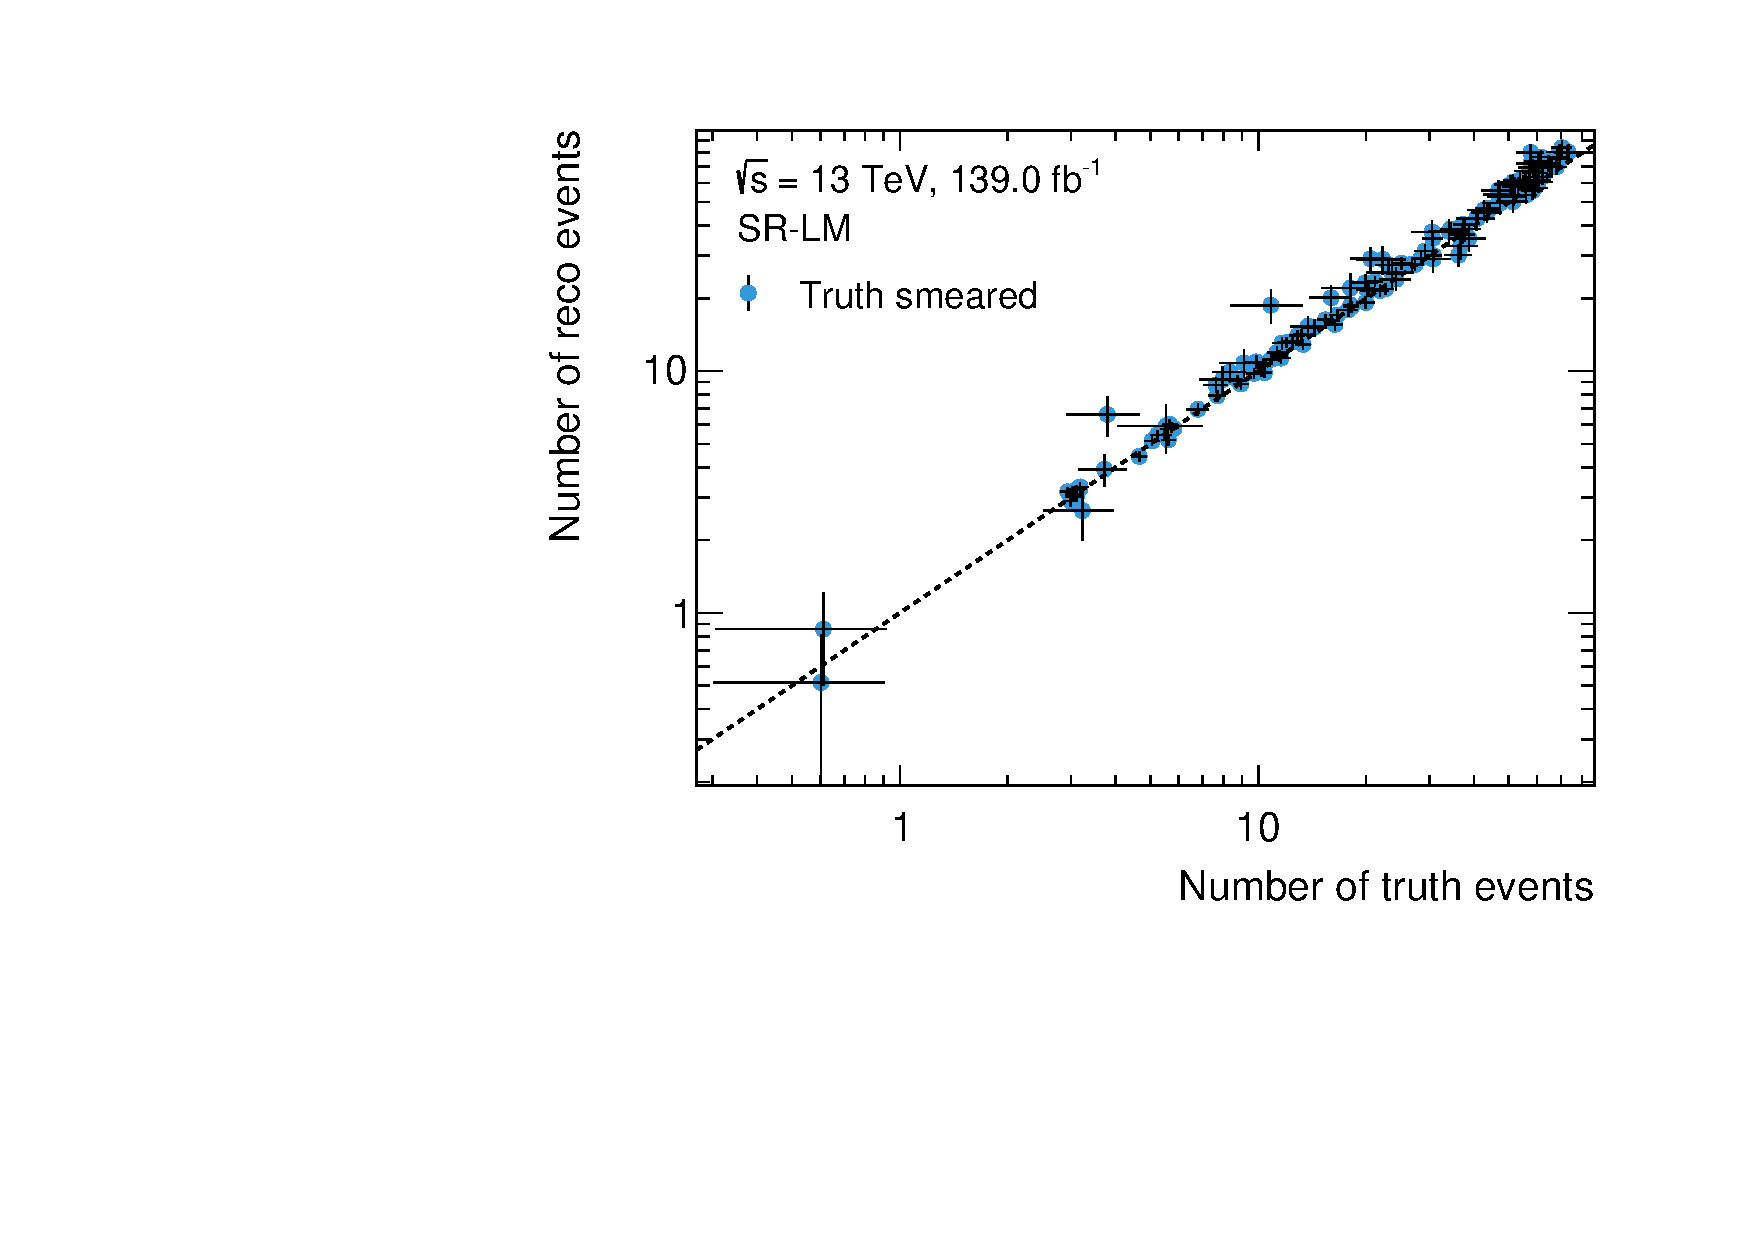
\includegraphics[width=\textwidth]{yields_SR-LM_smeared}
	\end{subfigure}\hfill
	\begin{subfigure}[b]{0.49\linewidth}
		\centering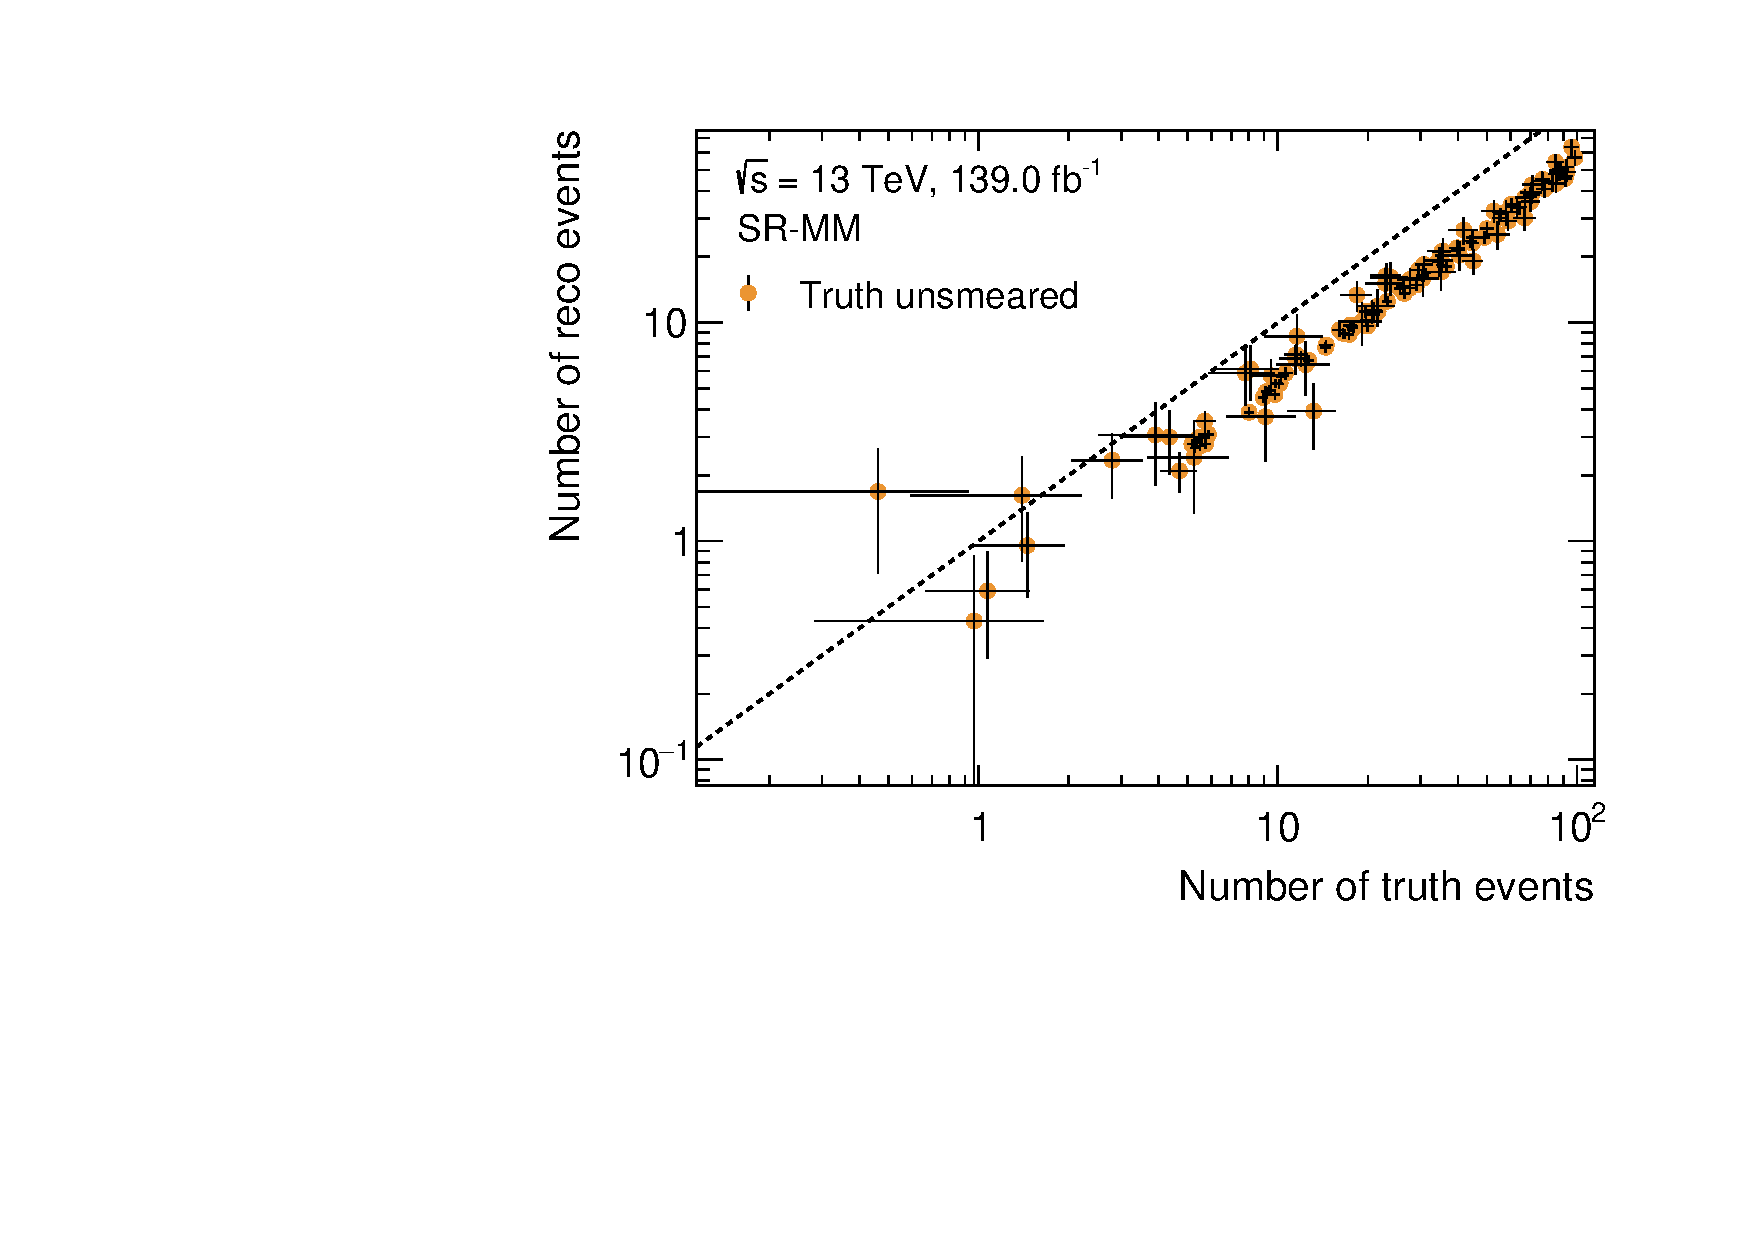
\includegraphics[width=\textwidth]{yields_SR-MM_unsmeared}
	\end{subfigure}\hfill
	\begin{subfigure}[b]{0.49\linewidth}
		\centering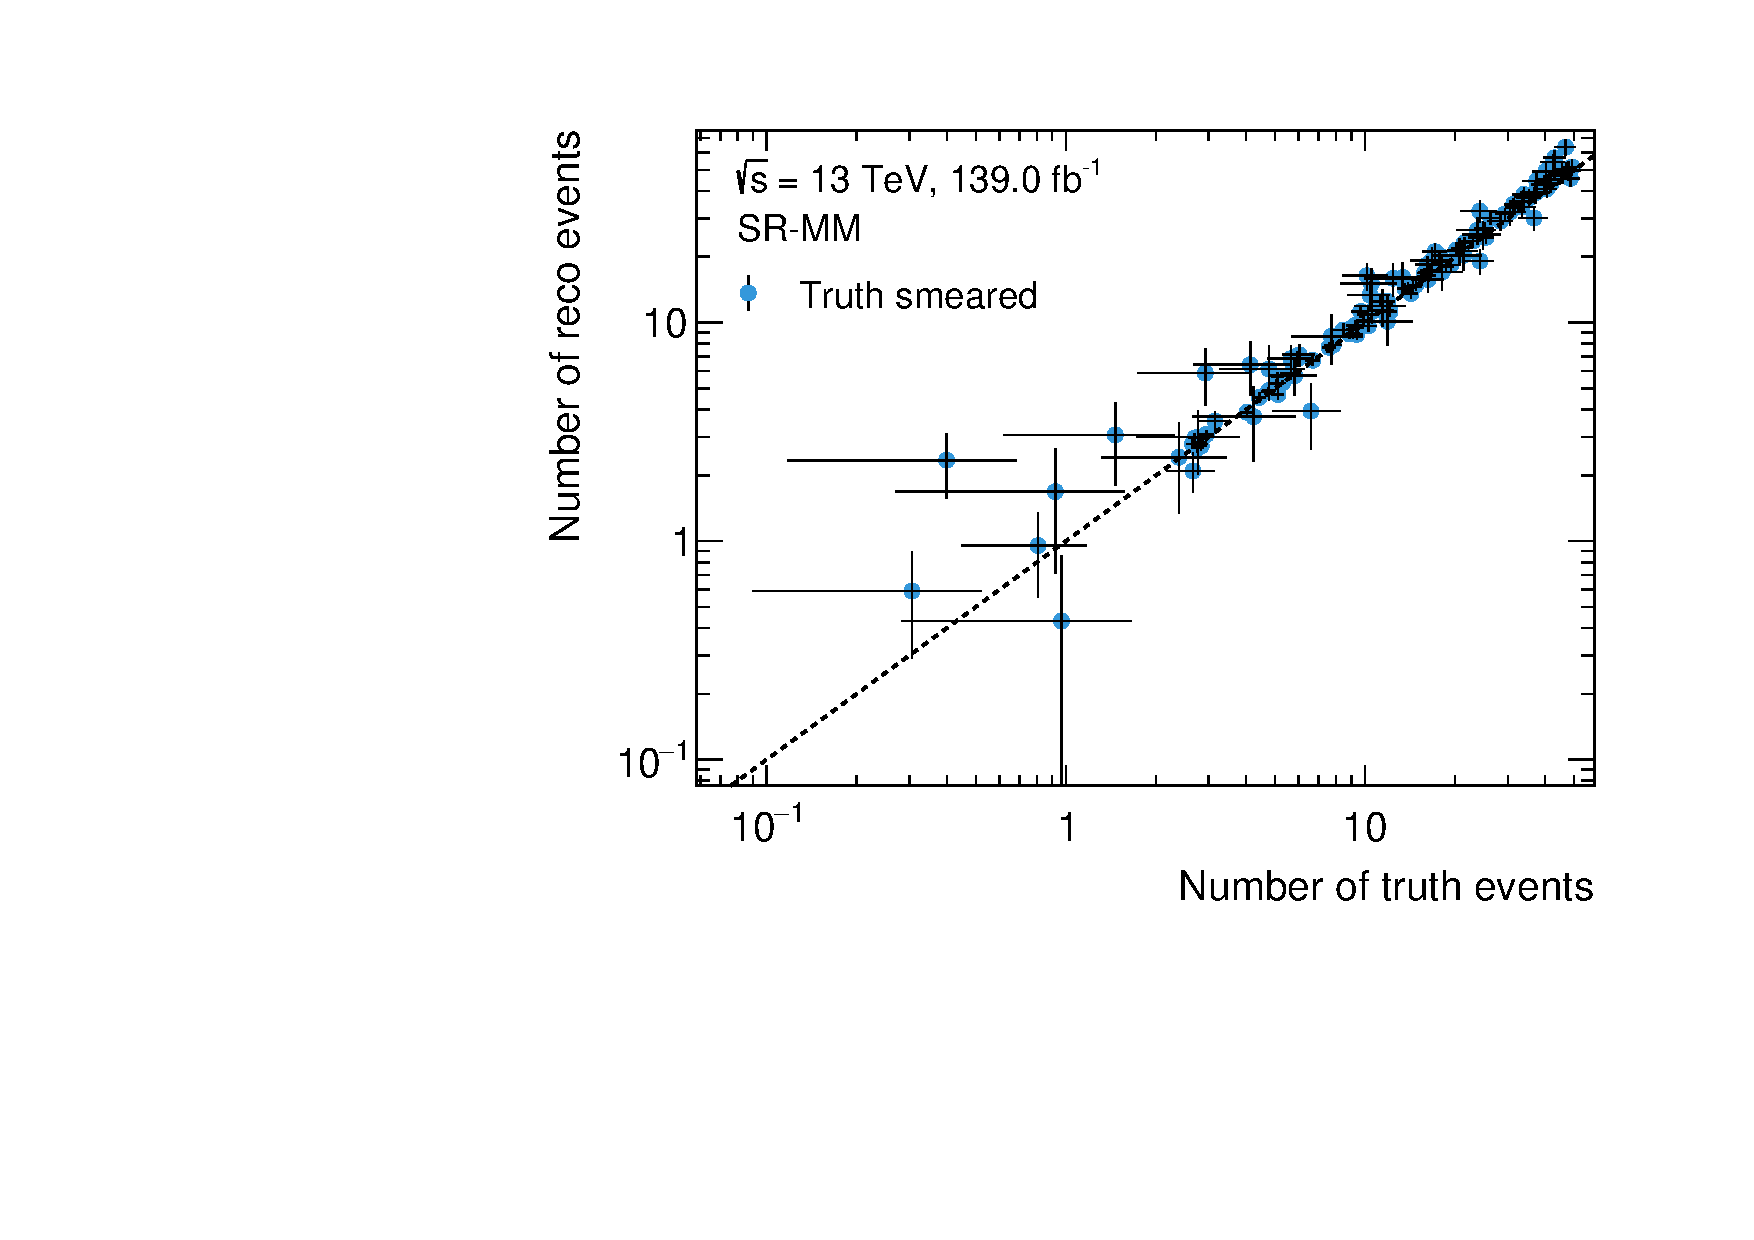
\includegraphics[width=\textwidth]{yields_SR-MM_smeared}
	\end{subfigure}\hfill
	\begin{subfigure}[b]{0.49\linewidth}
		\centering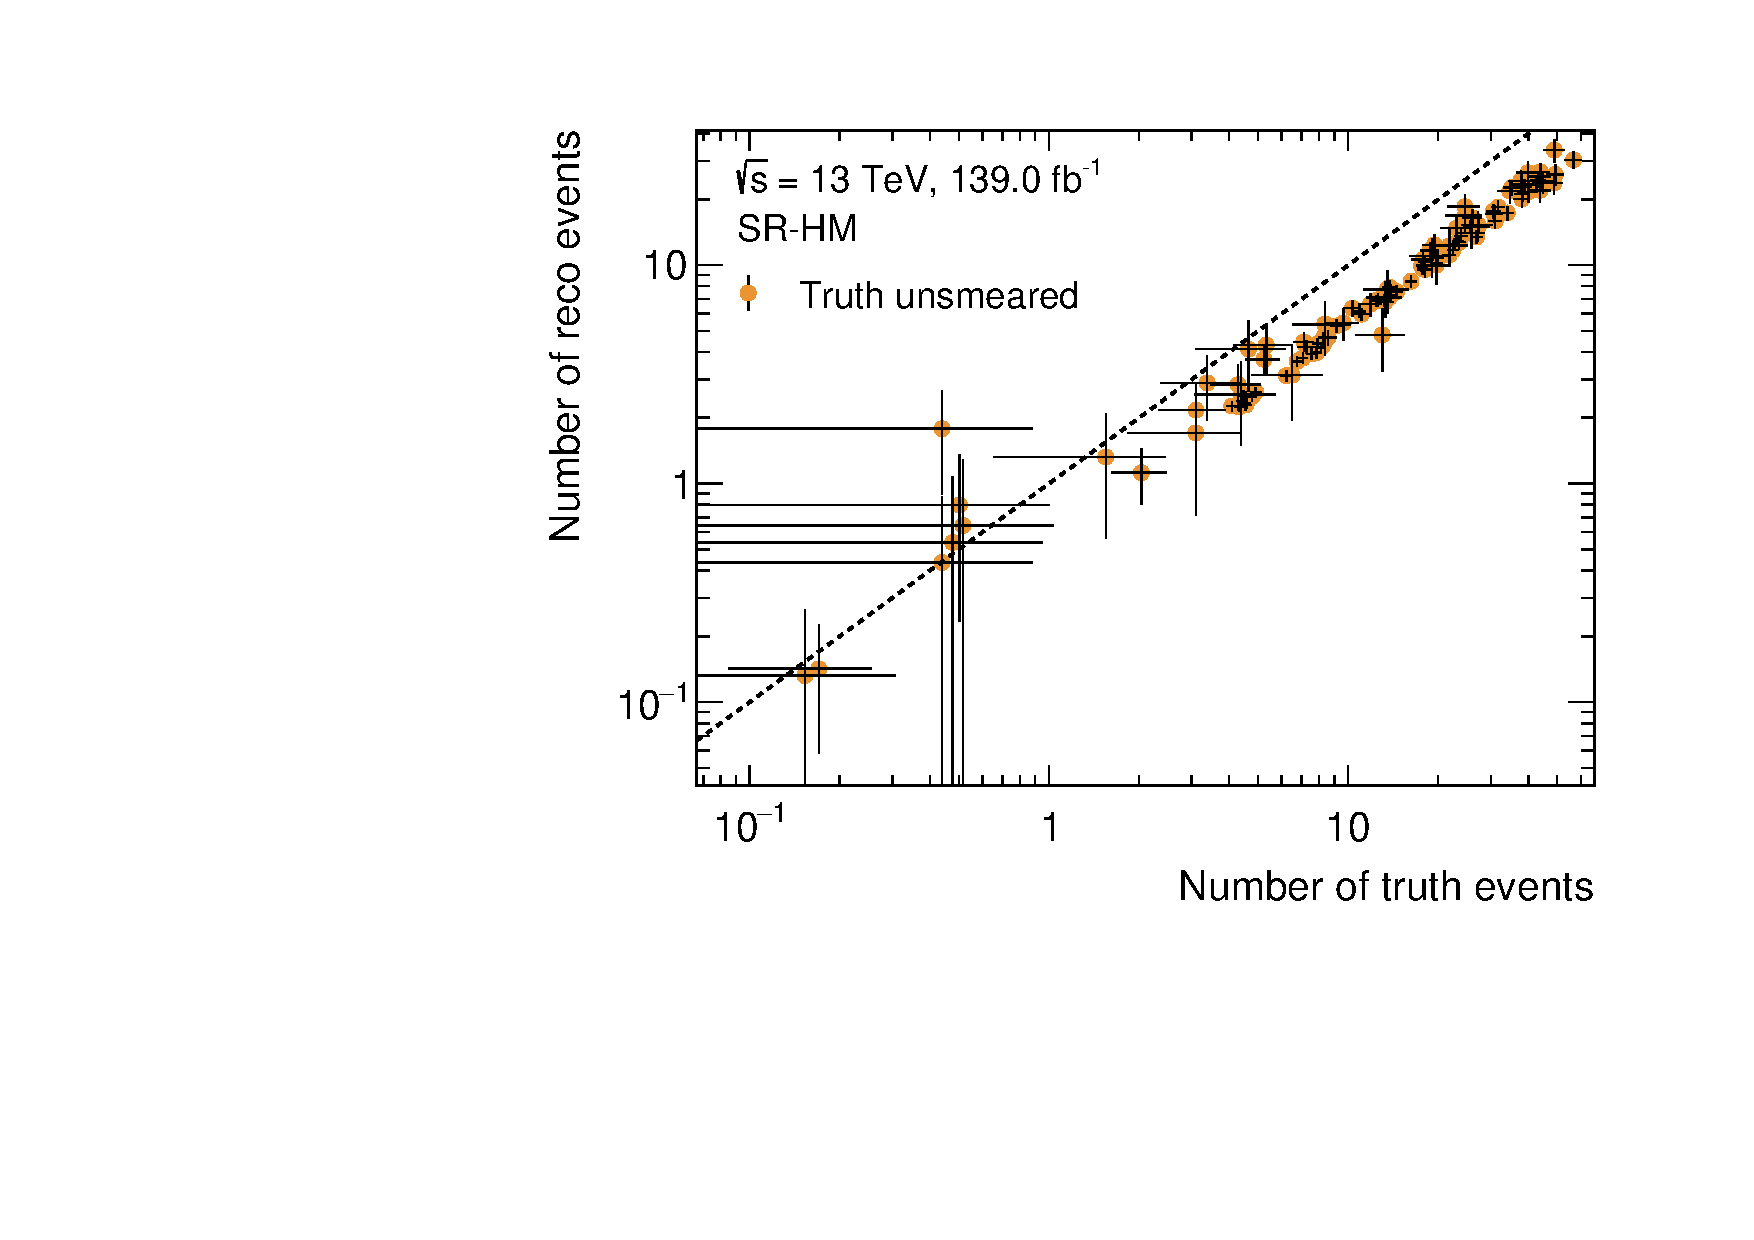
\includegraphics[width=\textwidth]{yields_SR-HM_unsmeared}
	\end{subfigure}\hfill
	\begin{subfigure}[b]{0.49\linewidth}
		\centering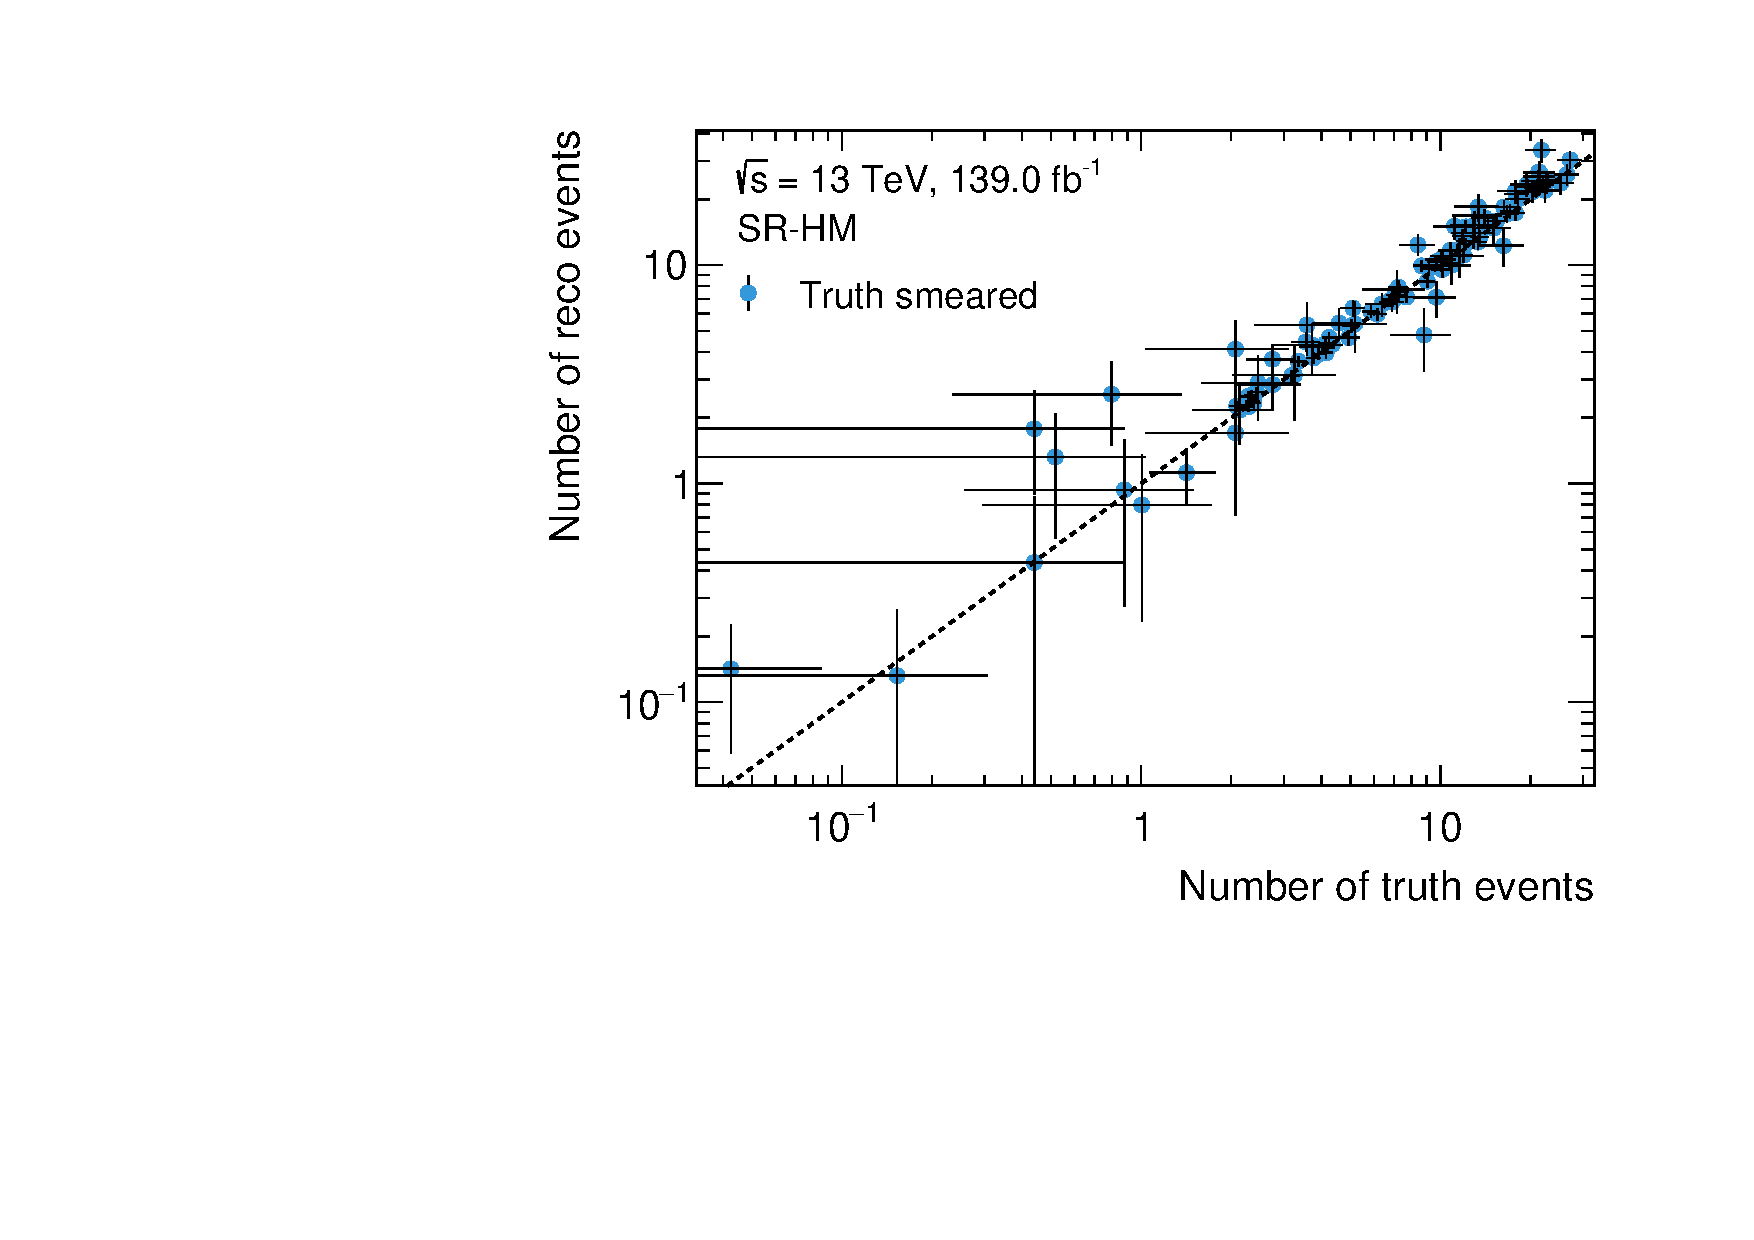
\includegraphics[width=\textwidth]{yields_SR-HM_smeared}
	\end{subfigure}
	\caption{Comparison of the event rates at truth- and reconstruction-level before (left) and after (right) truth smearing. From top to bottom, the SR-LM, SR-MM and SR-HM signal regions are shown, with cumulative (integrated) $\mct$ bins. Every single point in the scatter plots represents a single signal model considered in the original 1-lepton analysis. Uncertainties include \gls{mc} statistical uncertainties.}
	\label{fig:smearing_signal_regions}
\end{figure}
 
 As the expected signal rates in the signal regions are ultimately what is entering the (simplified) likelihood, it is important that the good agreement observed at preselection is still present in the kinematically tighter selections of the signal regions. Additionally, it is worth investigating the agreement across all signal models considered in the original analysis, as opposed to only validating specific benchmark points. A comparison of the reconstruction-level and truth-level event rates before and after smearing in the signal regions SR-LM, SR-MM and SR-HM is shown in~\cref{fig:smearing_signal_regions} for all signal models considered in the 1-lepton analysis. For the sake of conciseness, only the cumulative $\mct$ bins are shown in each \gls{sr} in~\cref{fig:smearing_signal_regions}. The agreement in the individual $\mct$ bins in each SR-LM, SR-MM and SR-HM is provided in~\cref{fig:smearing_signal_regions_1,fig:smearing_signal_regions_2,fig:smearing_signal_regions_3}.
 
The truth smearing drastically improves the agreement in event rate estimates at truth- and reconstruction-level across all \gls{sr} bins considered. While the event rates are generally overestimated at truth-level before smearing, compared to reconstruction-level, both tend to agree well within statistical uncertainties after smearing. 
 
\subsection{Validation using likelihood}


 \begin{figure}
	\centering
	\begin{subfigure}[b]{0.49\linewidth}
		\centering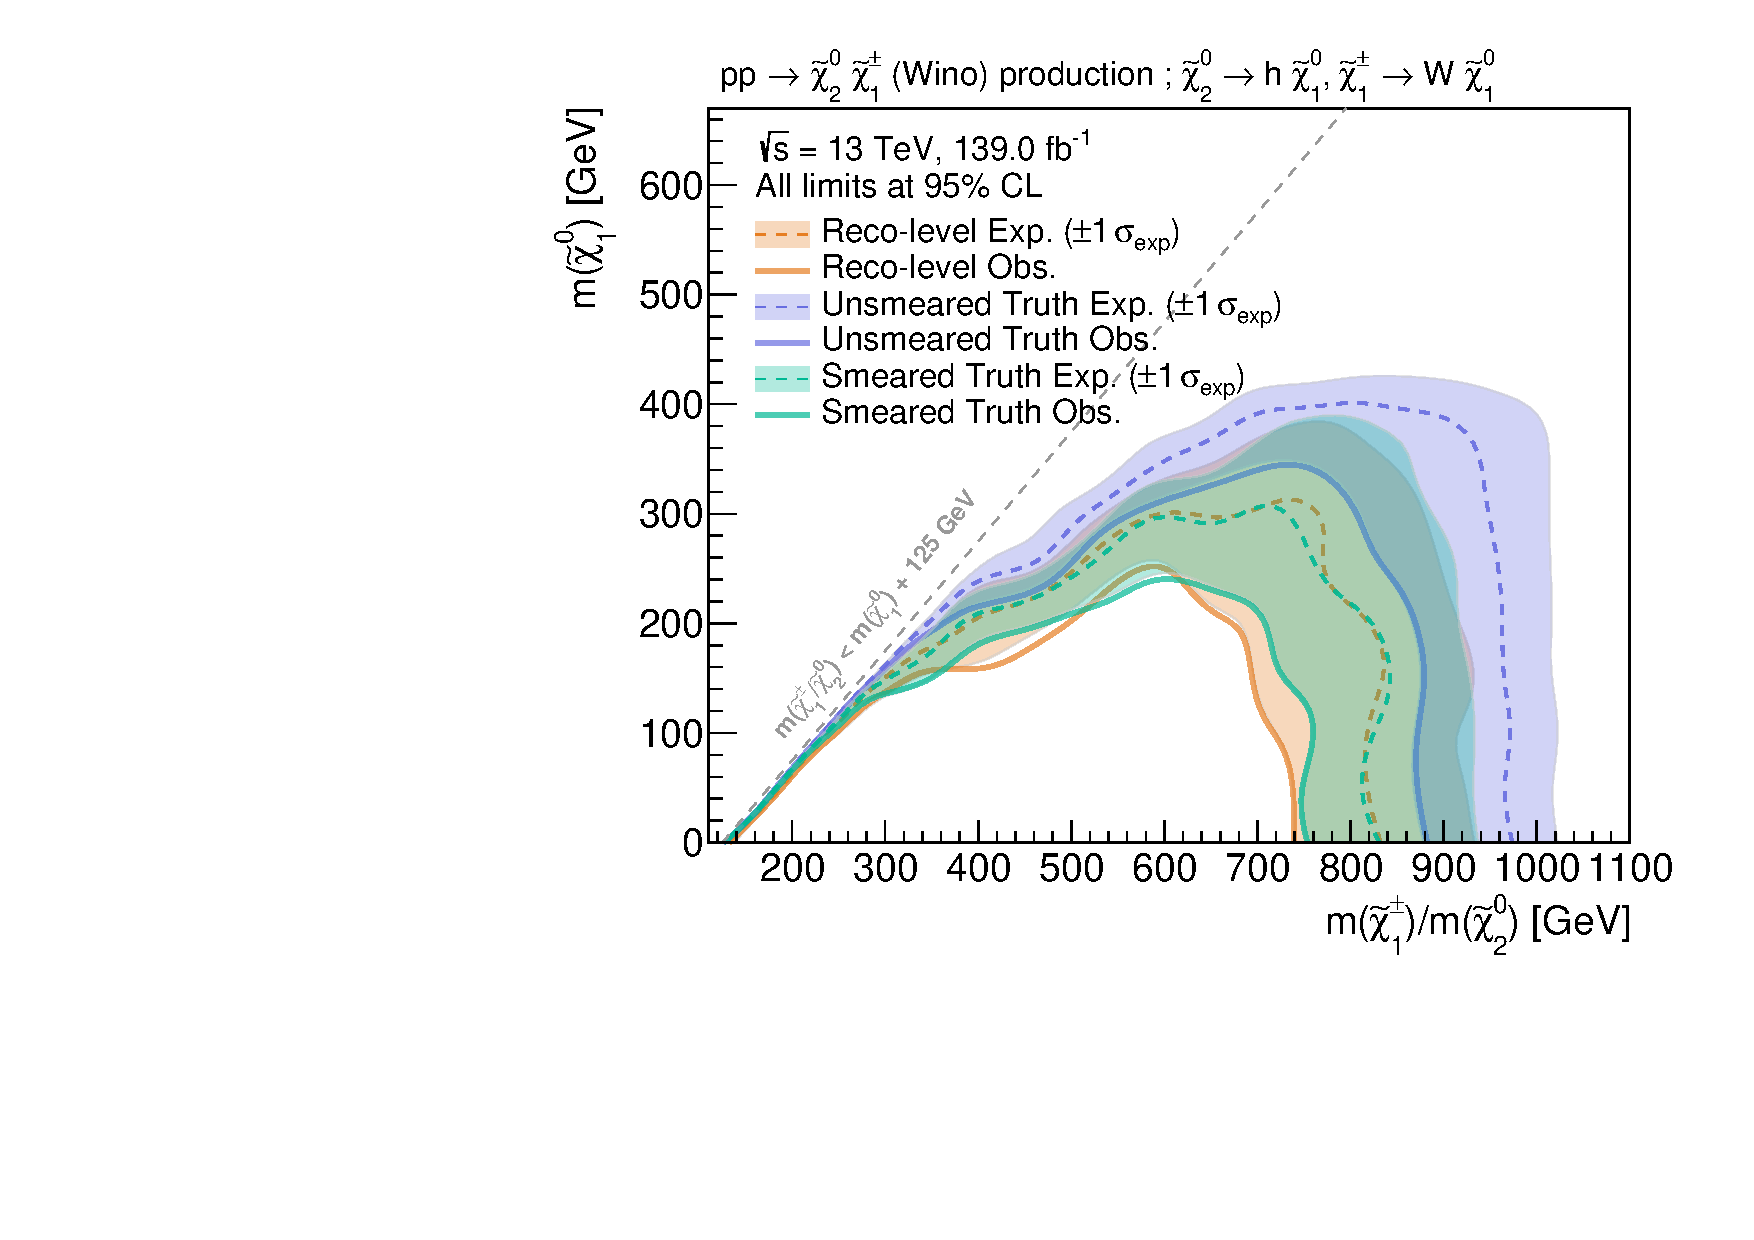
\includegraphics[width=\textwidth]{exclusion_1Lbb_truthInput_compareReco_BkgOnly_noLabel}
		\caption{\label{fig:full_truth_result}}
	\end{subfigure}\hfill
	\begin{subfigure}[b]{0.49\linewidth}
		\centering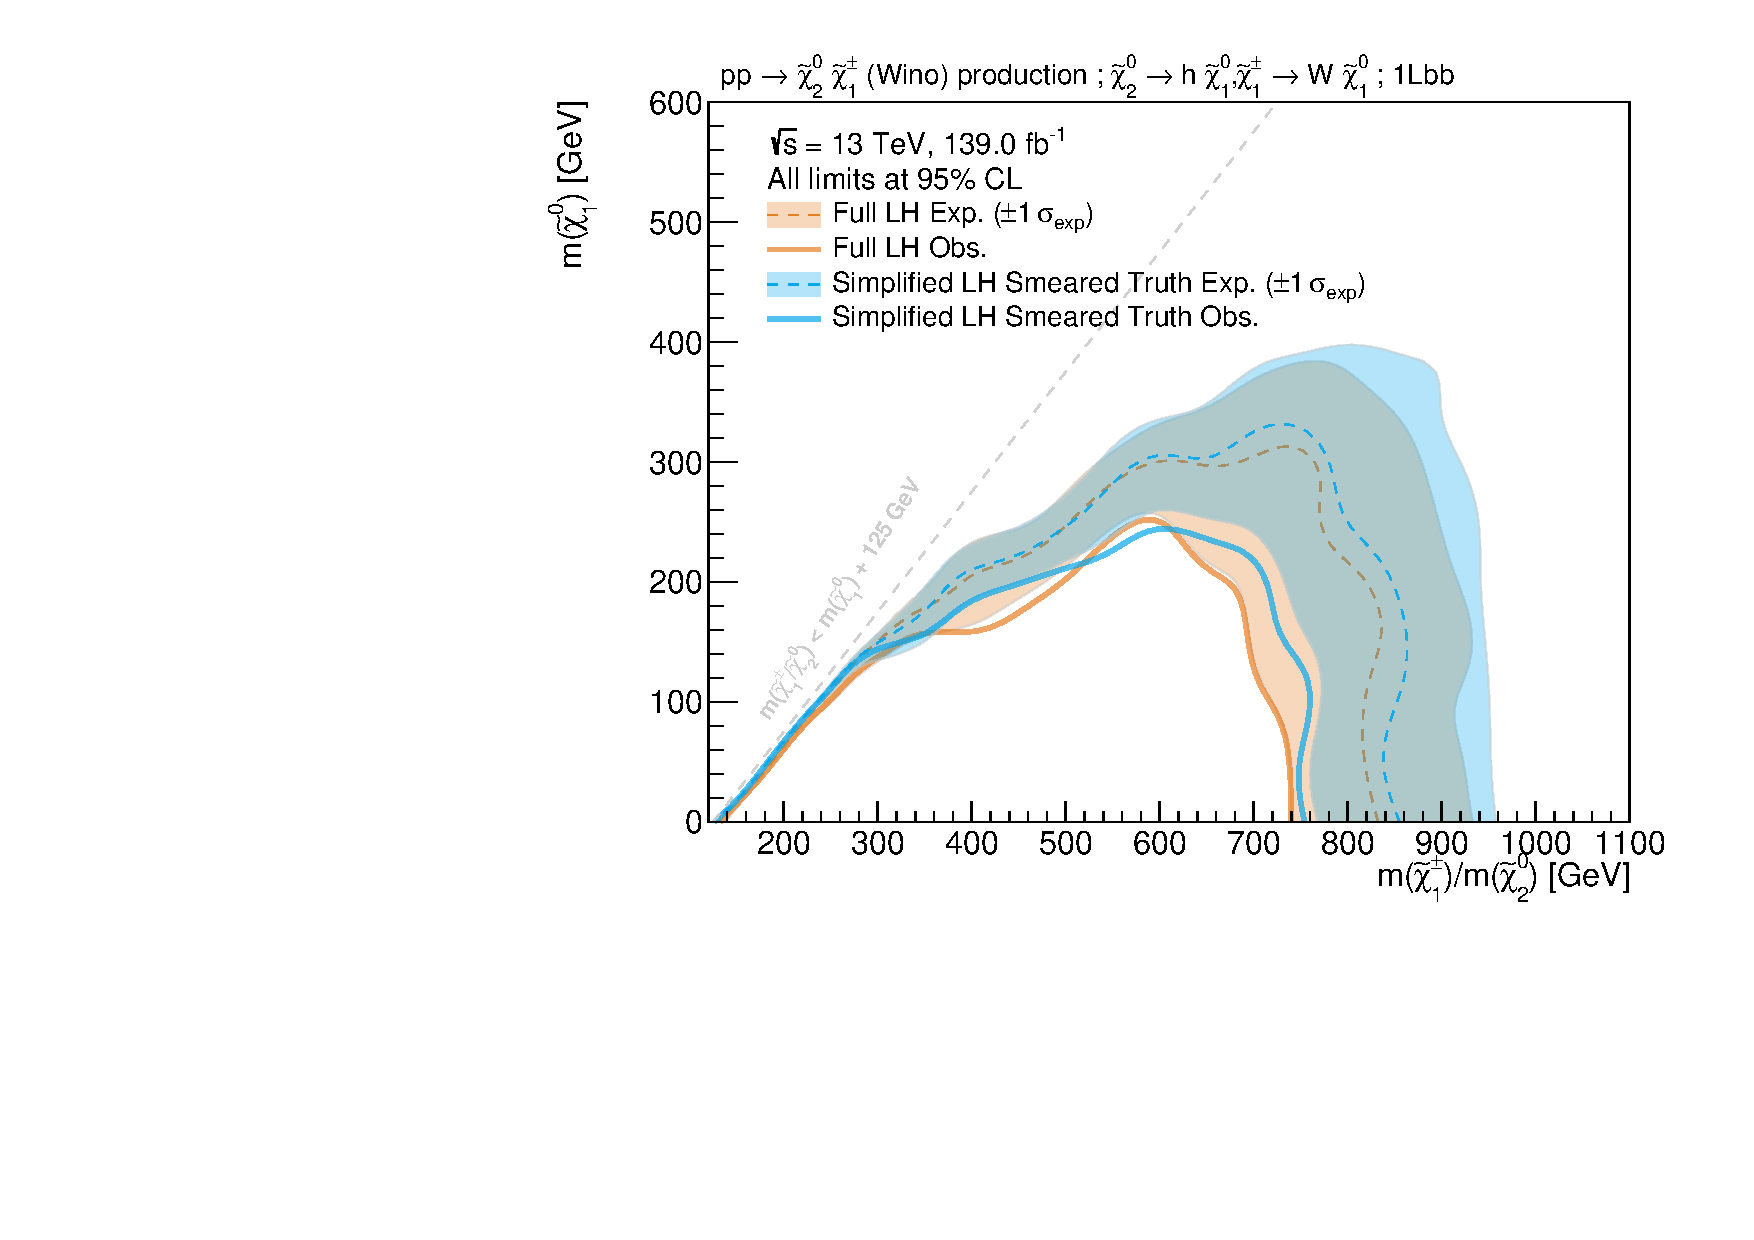
\includegraphics[width=\textwidth]{exclusion_1Lbb_truthInput_BkgSignal_700_200_noLabel}
		\caption{\label{fig:simplified_truth_result}}
	\end{subfigure}\hfill
	\caption{Expected and observed exclusion contours obtained with the full and simplified likelihoods. Fig.~\subref{fig:full_truth_result} compares the full likelihood contours obtained with the reconstruction-level inputs (orange) to results obtained with truth inputs before (purple) and after (green) smearing. Fig.~\subref{fig:simplified_truth_result} compares the full likelihood reconstruction-level contours (orange) with those obtained using the simplified likelihood and smeared truth-level inputs (blue). Uncertainties include all statistical and systematic uncertainties on the background and signal for the reconstruction-level contours, but only statistical and systematic uncertainties on the background for truth-level signal inputs.}
	\label{fig:smearing_signal_regions}
\end{figure}

Using the nominal expected event rates at smeared truth-level for every signal model in the original signal grid considered in the 1-lepton analysis, expected and observed CL$_s$ values can be computed and exclusion contours can be derived. \Cref{fig:full_truth_result} compares the expected and observed exclusion contours obtained using the full likelihood and reconstruction-level signal inputs with those obtained using the full likelihood and truth-level signal inputs before and after truth smearing. While all theory and systematic uncertainties on the signal are included in the reconstruction-level contours, no signal uncertainties are considered when obtaining both the smeared and unsmeared truth-level contours. As expected from the previous validation steps in the signal regions, the sensitivity using unsmeared truth-level signal inputs is significantly overestimated compared to the published analysis exclusion limit using reconstruction-level inputs. The smeared truth-level inputs, however, yield exclusion contours with an acceptable match compared to the reconstruction-level results.

With the truth smearing validated at multiple selection levels of the analysis, the full two-fold approximation of signal pipeline and statistical inference can be constructed. \Cref{fig:simplified_truth_result} compares the exclusion contours of the original analysis results with those obtained using smeared truth-level signal inputs as well as the simplified likelihood. Even with the approximations made, overall a good agreement is found and the original analysis results can be reproduced to a relatively high degree of precision.

In summary, this validation process shows that the signal pipeline in~\cref{fig:pipeline_analysis} can be efficiently approximated using truth-level analysis and a simplified treatment of the statistical model, allowing a considerably faster evaluation of \gls{bsm} models while still offering reliable results. In large-scale reinterpretations, this approach thus enables an efficient classification of models into safely excluded and non-excluded models as well as models where exclusion is in doubt and where the full analysis pipeline using \textsc{Recast} is needed.

\section{Model sampling and processing}\label{sec:pmssm_sampling}


\subsection{Sampling}

\begin{table}[h]
	\centering
	\small
	\caption{Scan ranges used for each of the 19 pMSSM parameters. For parameters written with a modulus sign, both the positive and negative values are allowed. The term ``gen(s)'' refers to generation(s).}
	\setlength\heavyrulewidth{0.2ex}
	\begin{tabular} {l r r l}
		\toprule
		Parameter & min & max & Note \\ 
		\midrule
		$m_{\tilde{L}_1}$ $(=m_{\tilde{L}_2})$ & $\SI{10}{\TeV}$ & $\SI{10}{\TeV}$ & Left-handed slepton (first two gens.) mass \\
		$m_{\tilde{e}_1}$ $(=m_{\tilde{e}_2})$ & $\SI{10}{\TeV}$ & $\SI{10}{\TeV}$ & Right-handed slepton (first two gens.) mass \\ 
		$m_{\tilde{L}_3}$ & $\SI{10}{\TeV}$ & $\SI{10}{\TeV}$ & Left-handed stau doublet mass \\
		$m_{\tilde{e}_3}$ & $\SI{10}{\TeV}$ & $\SI{10}{\TeV}$ & Right-handed stau mass \\
		\midrule
		$m_{\tilde{Q}_1}$ $(=m_{\tilde{Q}_2})$ & $\SI{10}{\TeV}$ & $\SI{10}{\TeV}$ & Left-handed squark (first two gens.) mass \\
		$m_{\tilde{u}_1}$ $(=m_{\tilde{u}_2})$ & $\SI{10}{\TeV}$ & $\SI{10}{\TeV}$ & Right-handed up-type squark (first two gens.) mass \\
		$m_{\tilde{d}_1}$ $(=m_{\tilde{d}_2})$ &$\SI{10}{\TeV}$ & $\SI{10}{\TeV}$ & Right-handed down-type squark (first two gens.) mass \\
		$m_{\tilde{Q}_3}$ & $\SI{2}{\TeV}$ & $\SI{5}{\TeV}$ & Left-handed squark (third gen.) mass \\
		$m_{\tilde{u}_3}$ & $\SI{2}{\TeV}$ & $\SI{5}{\TeV}$ & Right-handed top squark mass \\
		$m_{\tilde{d}_3}$ & $\SI{2}{\TeV}$ & $\SI{5}{\TeV}$ & Right-handed bottom squark mass \\
		\midrule
		$\vert M_1\vert$ & $\SI{0}{\TeV}$ & $\SI{2}{\TeV}$ & Bino mass parameter \\
		$\vert M_2\vert$ & $\SI{0}{\TeV}$ & $\SI{2}{\TeV}$ & Wino mass parameter \\
		$\vert\mu\vert$ & $\SI{0}{\TeV}$ & $\SI{2}{\TeV}$ & Bilinear Higgs mass parameter \\
		$M_3$ & $\SI{1}{\TeV}$ & $\SI{5}{\TeV}$ & Gluino mass parameter \\
		\midrule
		$\vert A_t\vert$ & $\SI{0}{\TeV}$ & $\SI{8}{\TeV}$ & Trilinear top coupling \\
		$\vert A_b\vert$ & $\SI{0}{\TeV}$ & $\SI{2}{\TeV}$ & Trilinear bottom coupling \\
		$\vert A_\tau\vert$ & $\SI{0}{\TeV}$ & $\SI{2}{\TeV}$ & Trilinear $\tau$ lepton coupling \\
		$M_A$ & $\SI{0}{\TeV}$ & $\SI{5}{\TeV}$ & Pseudoscalar Higgs boson mass \\
		$\tan\beta$ & $1$ & $60$ & Ratio of the Higgs vacuum expectation values \\
		\bottomrule
	\end{tabular}

	\label{fig:pmssm_scan_ranges}   
\end{table}

All signal models considered in the following are sampled from the \gls{pmssm} using the parameter ranges shown in~\cref{fig:pmssm_scan_ranges}. Flat probability distributions are used to draw random values within the given ranges for each parameter and each unique set of \gls{pmssm} parameters generated that way is referred to as an independent \gls{susy} model. 

As this work discusses a search for electroweakinos, the \gls{susy} models drawn from the \gls{pmssm} are sampled with a special focus on said supersymmetric particles. This is achieved by setting the mass parameters of the first and second generation squarks as well as those of the sleptons to values much higher than those accessible at \gls{lhc} energies, effectively decoupling them. For naturalness arguments, third generation squarks and the gluino are not strictly decoupled but set to sufficiently high values such as not to affect the electroweak sector too much. The lower and upper bounds on the 12 scanned parameters are chosen to yield a high density of models with electroweakino masses accessible at \gls{lhc} energies. 

Once a value for each of the 19 \gls{pmssm} parameters has been chosen, a number of publicly available software packages are executed in order to compute the properties of each model point. In a first step, \textsc{SPheno}~v4.0.5~\cite{spheno_1:2003um,spheno_2:2011nf} is used to calculate the spectrum of the sparticles. The result of \textsc{SPheno} is used to determine the masses and mixings of the Higgs bosons using \textsc{FeynHiggs}~v2.15.0~\cite{FeynHiggs:1998yj,FeynHiggs_1:2018qog,FeynHiggs_2:2013ria}. An additional \gls{susy} spectrum calculation is performed with \textsc{SoftSusy}~v4.1.8~\cite{softsusy:2001kg}. Although the masses, mixings and branching fractions from \textsc{SoftSusy} will not directly be used in the following, the program is still required to complete successfully in order to reduce the number of \gls{pmssm} models with pathological properties. After the complete model spectrum has calculated, additional properties are determined. The dark matter relic abundance of each model is calculated with \textsc{micrOMEGAs}~v5.0.8~\cite{micromegas_1:2006is,micromegas_2:2010pz}. Finally, flavour physics and precision electroweak observables like $\Delta\rho$, $\Delta(g-2)_\mu$, $\mathrm{BR}(b\rightarrow s\gamma)$ and $\mathrm{BR}(B_s\rightarrow \mu^+\mu^-)$ are determined using  \textsc{SuperIso}~v4.0~\cite{superiso:2008tp}.

%\textsc{GM2Calc}~v1.7.1~\cite{gm2:2015rva} and

\subsection{Selection and processing}

In order to avoid models with pathological properties, all spectrum generators are required to finish execution without error. The cross section for surviving models is computed at \gls{nlo} using \textsc{Prospino}~v2.1~\cite{prospino:314229, prospino_2:1999xh}. Models with an inclusive cross sections for all electroweak production processes below $\SI{0.07}{\femto\barn}$ are discarded as they would result in less than 10 expected signal events with an integrated luminosity of \onethirtynineifb, not enough to be sensitive to with current electroweak \gls{susy} searches. 
%For the sake of experimental sensitivity, models are also required to have a lightest chargino with mass below $\SI{1.2}{\TeV}$ and produce a neutralino \gls{lsp}. 
Finally, models with long-lived or even stable (on the time scale needed for traversing the ATLAS detector) sparticles\footnote{Not considering the \gls{lsp}.} are discarded as \gls{susy} searches targeting prompt electroweakino decays (like the 1-lepton search), are not expected to be sensitive to these models. 

%As only $R$-parity conserving models are considered, the \gls{lsp} is stable and thus has a non-vanishing cosmological abundance. The resulting \gls{lsp} abundance is calculated but no upper limit is required in order to allow   required to be below the experimentally observed value of the cold dark matter relic density of $\Omega_c h^2 = 0.12$, thus not making a statement about whether or not the \gls{lsp} is the only \gls{dm} particle. 
No constraints on the computed cosmological \gls{lsp} abundance and precision electroweak and flavour observables are applied at this stage in order to give a more general view after the models are evaluated using the \onelepton search. Experimental constraints from \eg \gls{lep} are also not applied at this stage. 

Of the \num[group-separator={,}]{10000} unique models sampled from the \gls{pmssm} using the above prescription, \num[group-separator={,}]{5152} models survive the constraints and requirements discussed in this section and are analysed using the \onelepton search. The majority of the models rejected due to the cross section constraints.

\subsection{Event generation}

Event generation is performed using the software centrally provided by the ATLAS production system. The initial pair of sparticles with two one parton in the \gls{me} are generated using the \textsc{MadGraph5\_aMC@NLO} v2.6.1.~\cite{MGaMCNLO:2014hca,Frederix:2012ps} generator. Next, \textsc{Pythia8.230}~\cite{Pythia8:2007gs}  with the \textsc{A14} tune is used for the hadronisation and \gls{ps}, together with the NNPDF 2.3 LO~\cite{Ball:2012cx} \gls{PDF} set. The number of events generated scales with the cross section of the model, starting at $10^4$ and capping out at $10^6$ truth-level events.
		
\subsection{Truth-level analysis}

All models passing event generation are evaluated using the truth-level analysis described in~\cref{sec:truth_analysis}. This is the only evaluation done for the models considered in this work. A full scan over the \gls{pmssm} including multiple ATLAS \gls{susy} searches would most likely include an additional processing step reverting to reconstruction-level analysis including the original analysis pipelines and full detector reconstruction for model points where (non-)exclusion is uncertain based on truth-level analysis only.

\section{Phenomenology of the LSP}\label{sec:lsp_pheno}

The composition of the $\lsp$ in each \gls{pmssm} model sampled is shown in the $m(\charg)$--$m(\lsp)$ and $m(\neutr)$--$m(\lsp)$ plane in~\cref{fig:lsp_types,fig:lsp_types_N2}, respectively. The $\lsp$ is considered to be bino-like ($\tilde{B}$-like), wino-like ($\tilde{W}$-like) or higgsino-like ($\tilde{H}$-like) if the corresponding fraction from the neutralino mass mixing matrix is at least 80\%. If more than one component has a fraction of more than 20\%, then the $\lsp$ is considered to be of mixed nature. 

In the bulk of the $m(\charg)$--$m(\lsp)$ plane, \ie the parameter space targeted by the \onelepton search using the simplified model, the large majority of the models produce a bino-like \gls{lsp} with nearly mass-degenerate $\charg$ and $\neutr$. These models correspond to cases where $M_1 \ll M_2, \mu$ and are closest to the canonical simplified model considered in the \onelepton search. Some sensitivity can be expected towards these models using the \onelepton search, provided that the branching fractions of the decays $\charg \rightarrow W^\pm \lsp$ and especially $\neutr \rightarrow h \lsp$ are large enough and produce on-shell bosons.

Towards the diagonal of $m(\charg)$--$m(\lsp)$ plane, \ie for models where the $\charg$ and $\lsp$ are nearly mass-degenerate, the nature of the \gls{lsp} shows a larger variation. In a large set of models, the \gls{lsp} has a significant wino component, leading to a mass spectrum where the $\charg$ and $\lsp$ are nearly mass-degenerate while the mass of the $\neutr$ can take on higher values. In models where the \gls{lsp} has a large higgsino component, \ie $\mu \ll M_1, M_2$, all three sparticles ($\charg$, $\neutr$ and $\lsp$) are nearly mass-degenerate and result in very soft decay products, making these models inherently difficult to target.

 \begin{figure}
	\centering
	\begin{subfigure}[b]{0.5\linewidth}
		\centering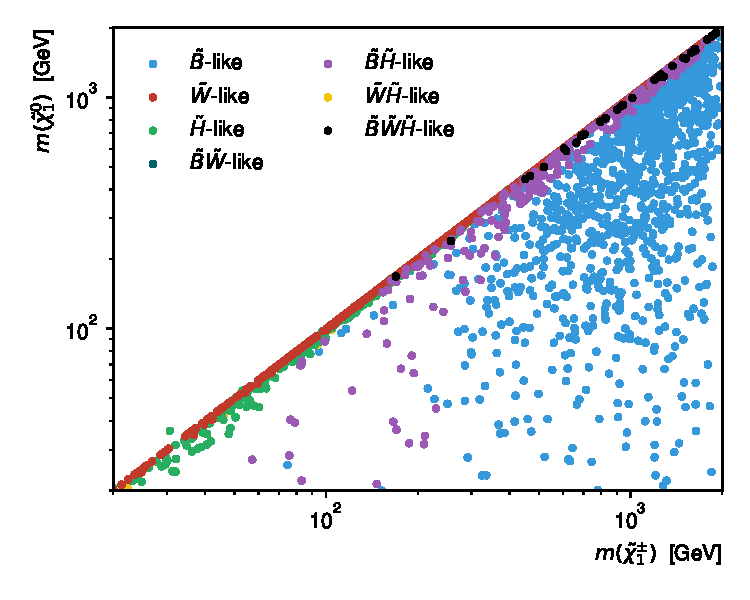
\includegraphics[width=\textwidth]{scatter/lsp_types.pdf}
		\caption{\label{fig:lsp_types}}
	\end{subfigure}\hfill
	\begin{subfigure}[b]{0.5\linewidth}
		\centering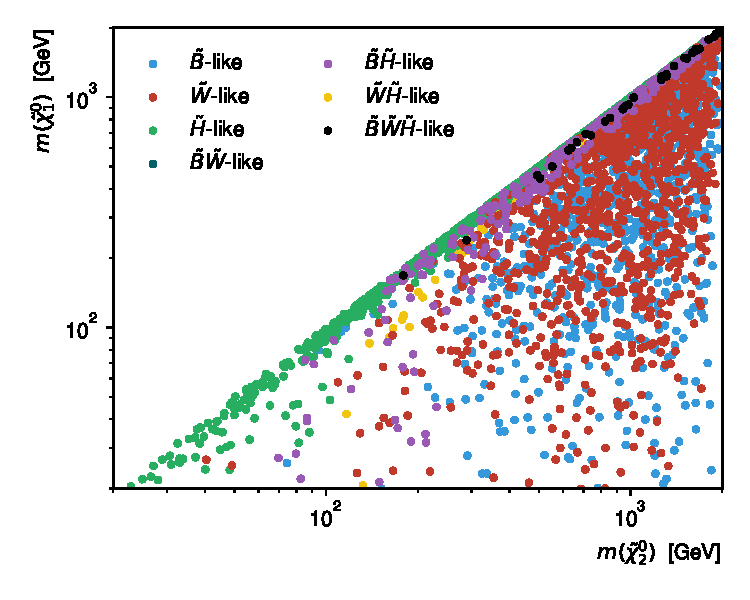
\includegraphics[width=\textwidth]{scatter/lsp_types_N2.pdf}
		\caption{\label{fig:lsp_types_N2}}
	\end{subfigure}\hfill
	\caption{Scatter plot of all models sampled in the \subref{fig:lsp_types} $m(\charg)$--$m(\lsp)$ and \subref{fig:lsp_types_N2} $m(\neutr)$--$m(\lsp)$ planes. The colour encodes the composition of the $\lsp$ in each model. The $\lsp$ is considered to be bino-like ($\tilde{B}$-like), wino-like ($\tilde{W}$-like) or higgsino-like ($\tilde{H}$-like) if the corresponding fraction from the neutralino mass mixing matrix is at least 80\%. Additionally, the $\lsp$ is considered to be of mixed nature if more than one component has a fraction of 20\%. For example, a $\tilde{B}\tilde{W}$-like $\lsp$ has more than 20\% bino and wino components, but less than 20\% higgsino component.}
	\label{fig:lsp_phenomenology}
\end{figure}

\section{Impact of the 1-lepton search on the pMSSM}

The impact of the 1-lepton search on the \gls{pmssm} is discussed using one-dimensional and two-dimensional distributions in the following sections. As usual, a model is considered to be excluded if the observed CL$_s$ value obtained from the simplified likelihood using the smeared truth-level inputs is below 0.05. Of the 7264 models evaluated, the \onelepton search excludes a total of 98, or about 1.3\%, of the models.

For the one-dimensional distributions shown in the following, the total number of models is compared against the number of models excluded by the \onelepton search. An additional pad indicates the ratio between models excluded and total models sampled in each bin of the distribution. In the two-dimensional distributions, the numbers in the bins indicate the number of \gls{pmssm} models falling into each respective bin. In these distributions, the fraction of models excluded with the \onelepton search is encoded using the $z$-axis, represented by a colour bar.

\subsection{Impact on electroweakino masses}

 \begin{figure}
	\centering
	\begin{subfigure}[b]{0.5\linewidth}
		\centering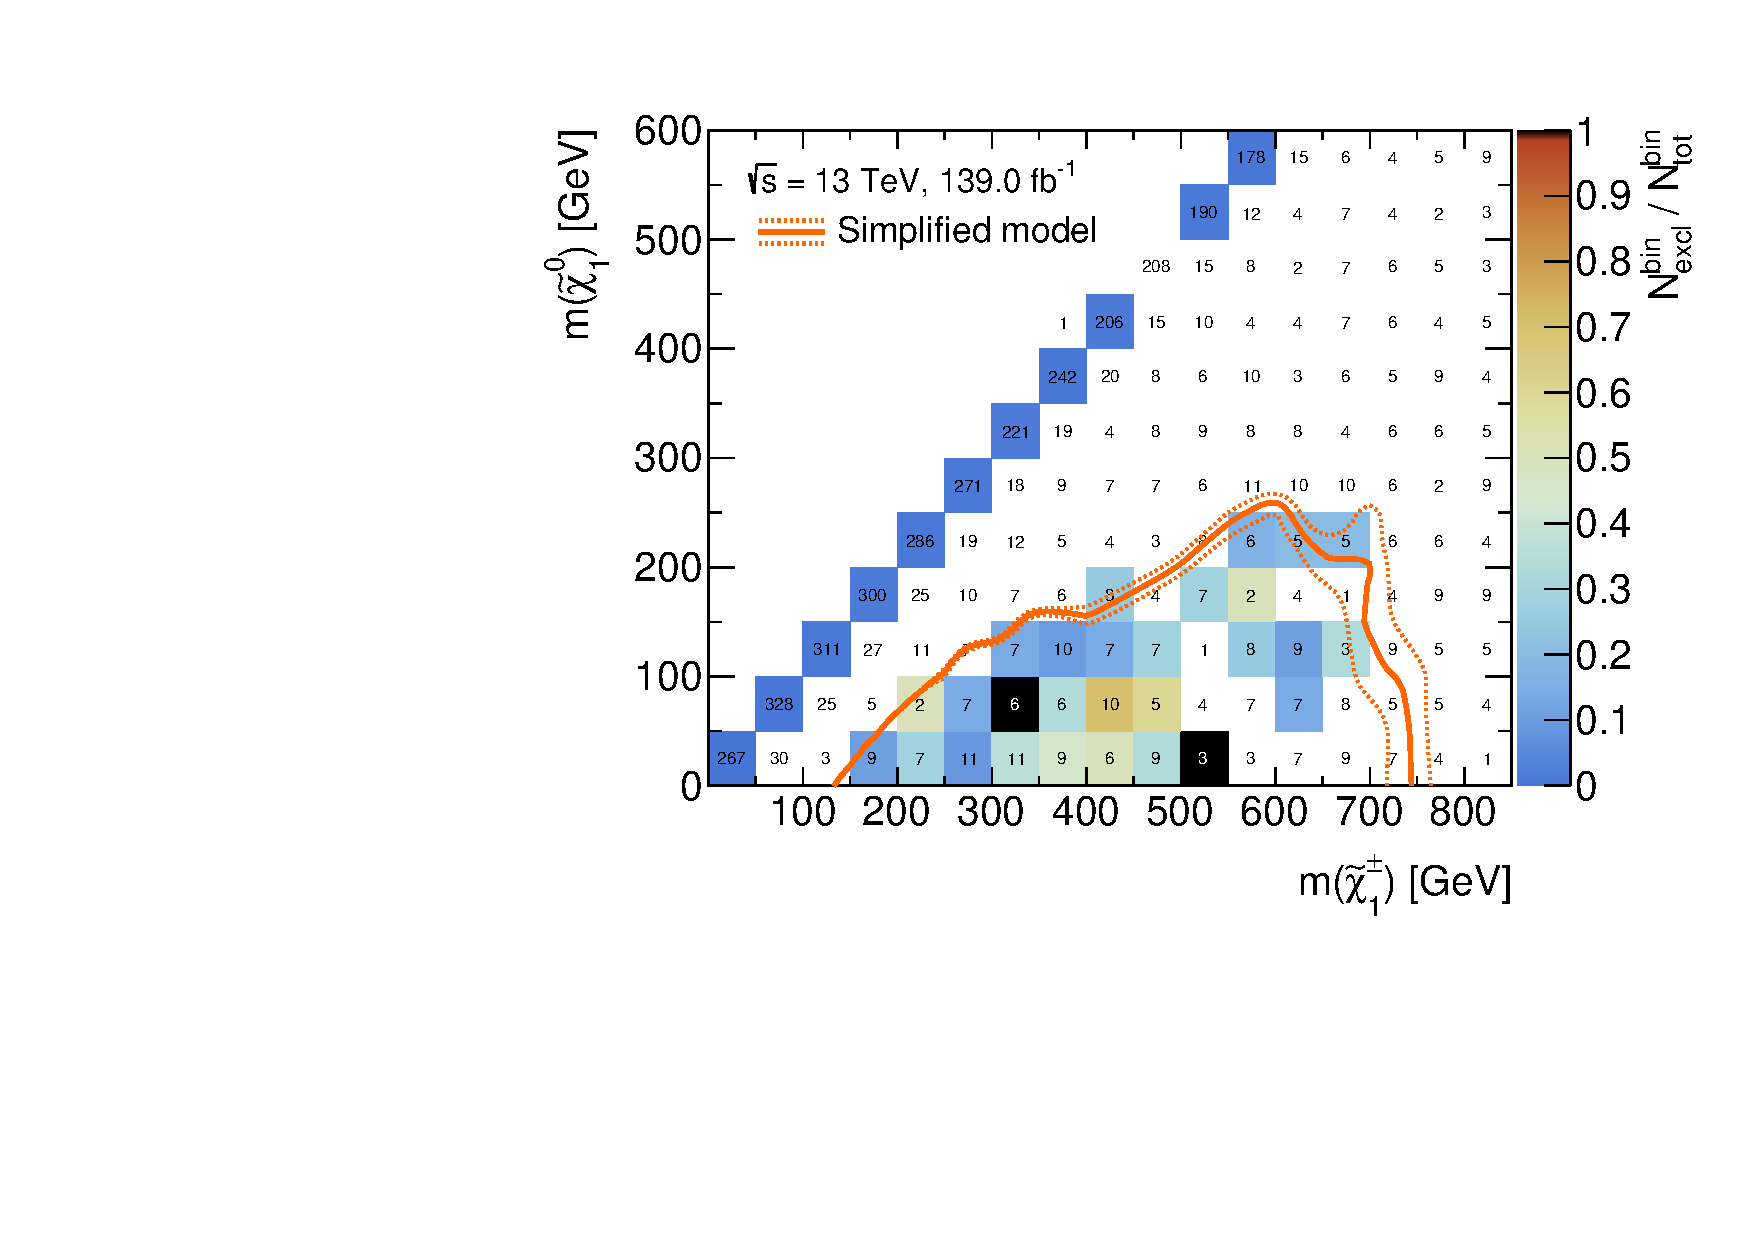
\includegraphics[width=\textwidth]{cut_none/mchi1p_mlsp_contour}
		\caption{\label{fig:mchi1p_mlsp_contour}}
	\end{subfigure}\hfill
	\begin{subfigure}[b]{0.5\linewidth}
		\centering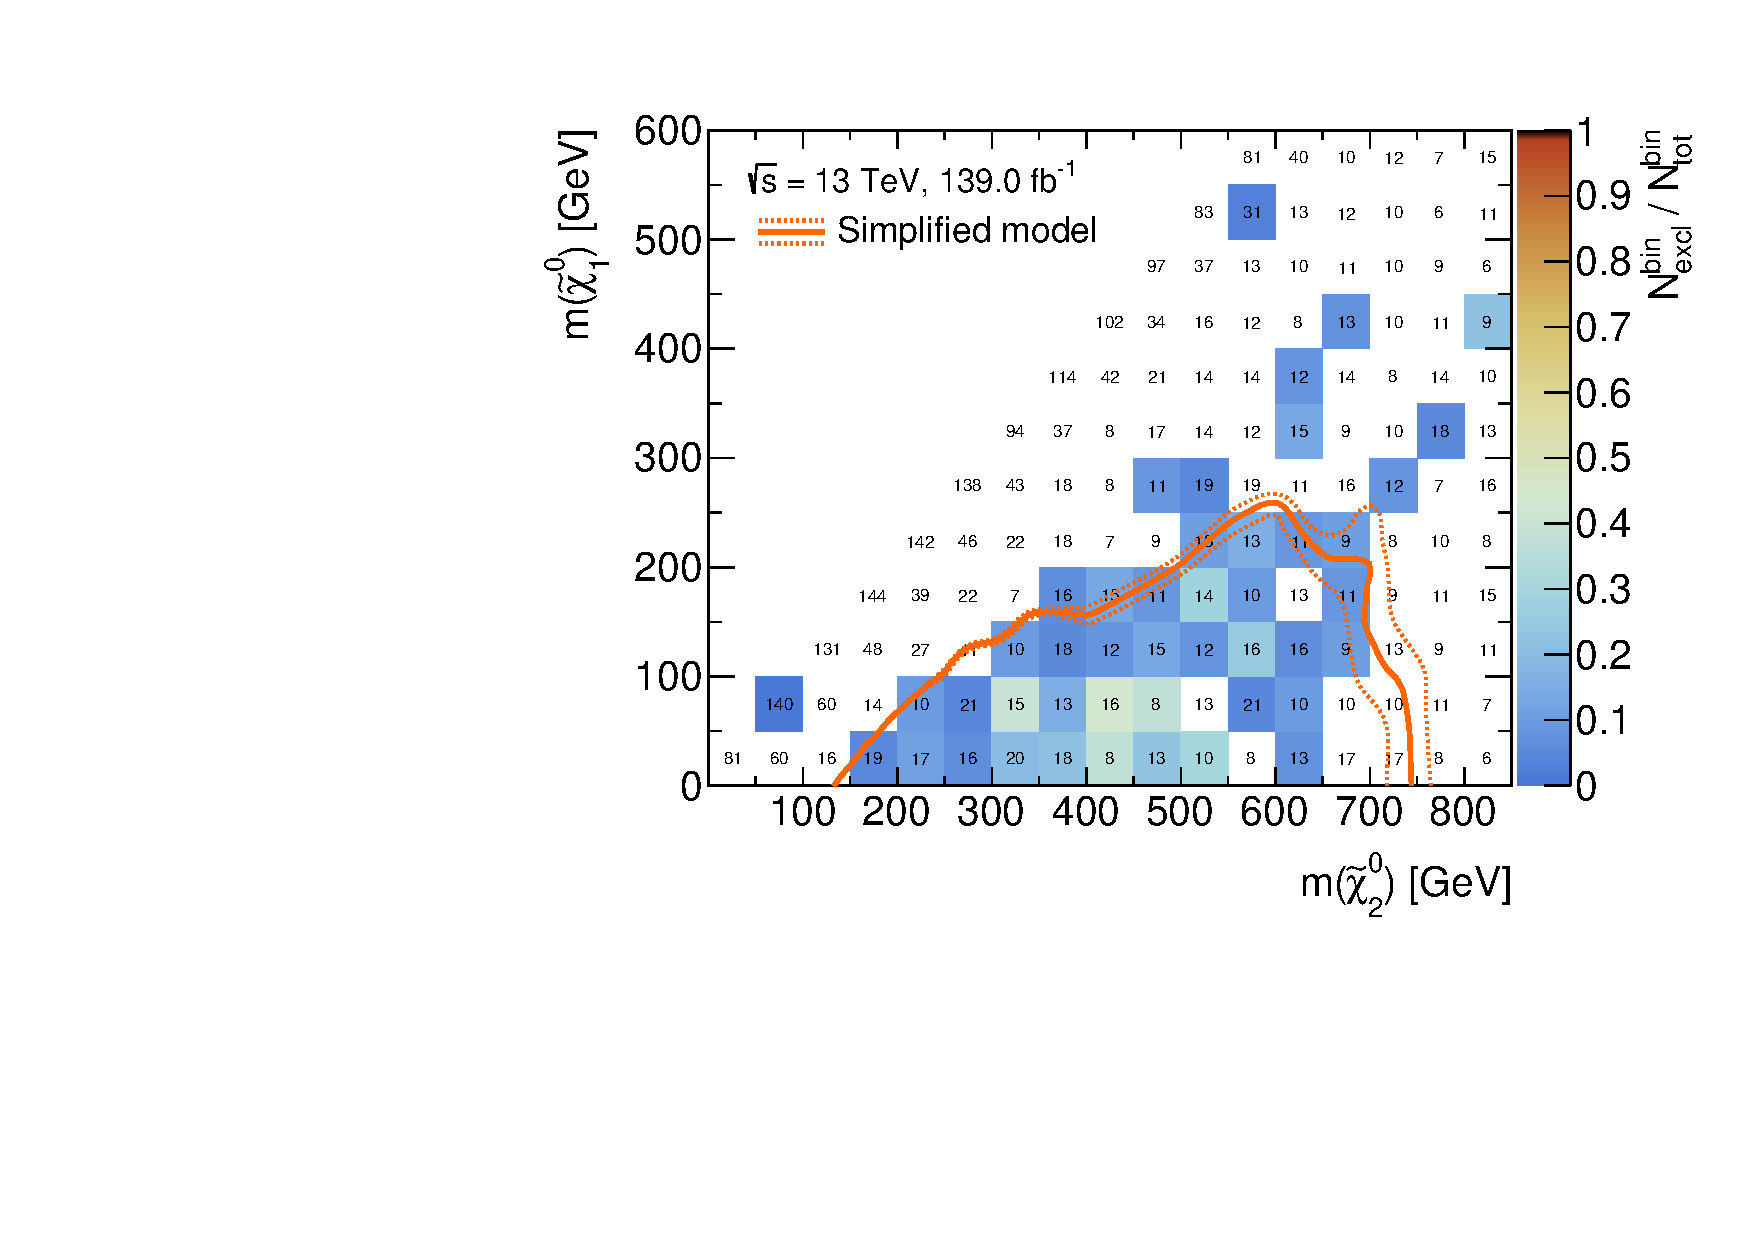
\includegraphics[width=\textwidth]{cut_none/mchi20_mlsp_contour}
		\caption{\label{fig:mchi20_mlsp_contour}}
	\end{subfigure}\hfill
	\begin{subfigure}[b]{0.5\linewidth}
		\centering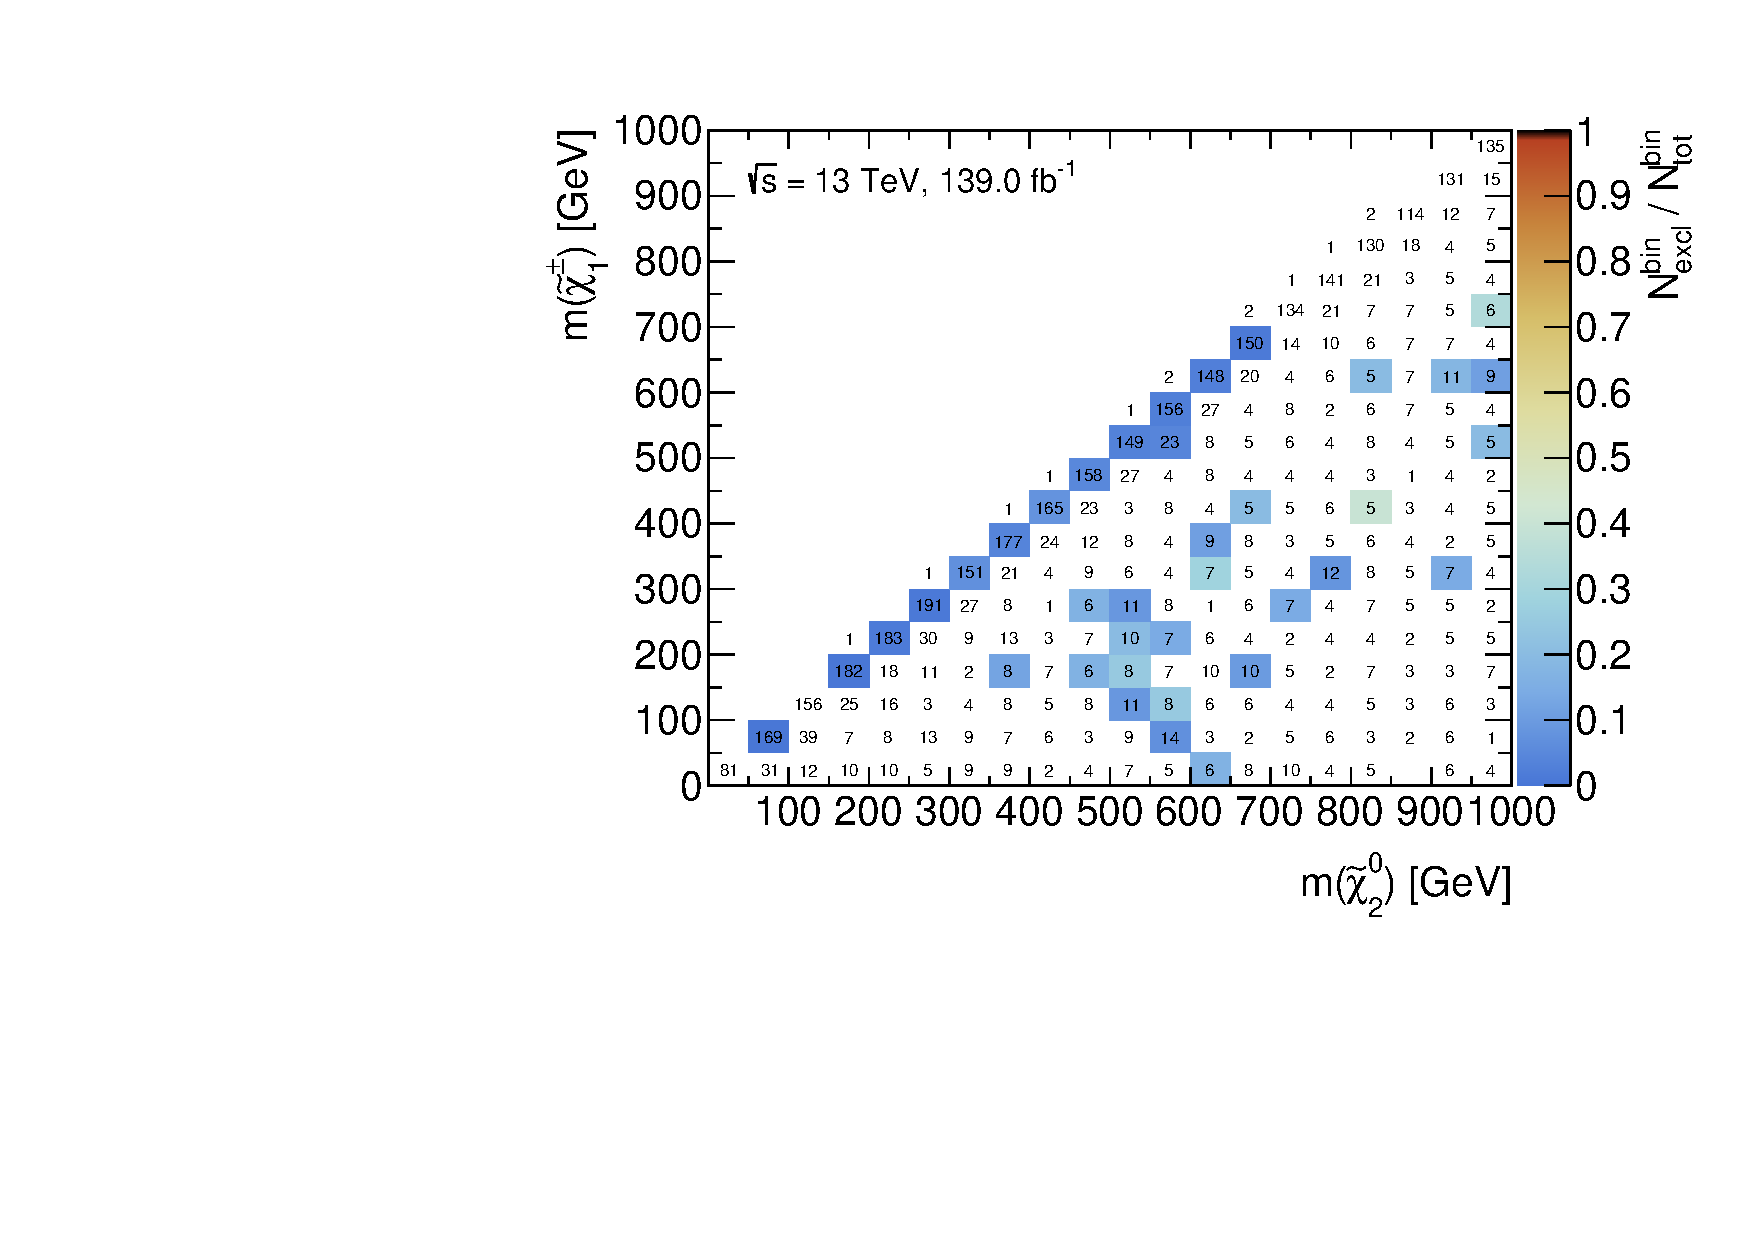
\includegraphics[width=\textwidth]{cut_none/mchi1p_mchi20_contour}
		\caption{\label{fig:mchi1p_mchi20_contour}}
	\end{subfigure}\hfill
	\caption{Bin-by-bin fraction of excluded models as a function of the relevant sparticle masses. The numbers in the bins correspond to the total number of models sampled falling into the respective bin. The number of models excluded by the 1-lepton analysis is encoded with a colour bar ranging from 0 to 1. Where all models in a given bin are excluded, the bin is coloured in black. Bins without any models excluded are left white. Models are evaluated using the simplified likelihood of the 1-lepton analysis. The simplified model contour is shown in orange.}
	\label{fig:impact_electroweakinos_2D}
\end{figure}


 \begin{figure}
	\centering
	\begin{subfigure}[b]{0.5\linewidth}
		\centering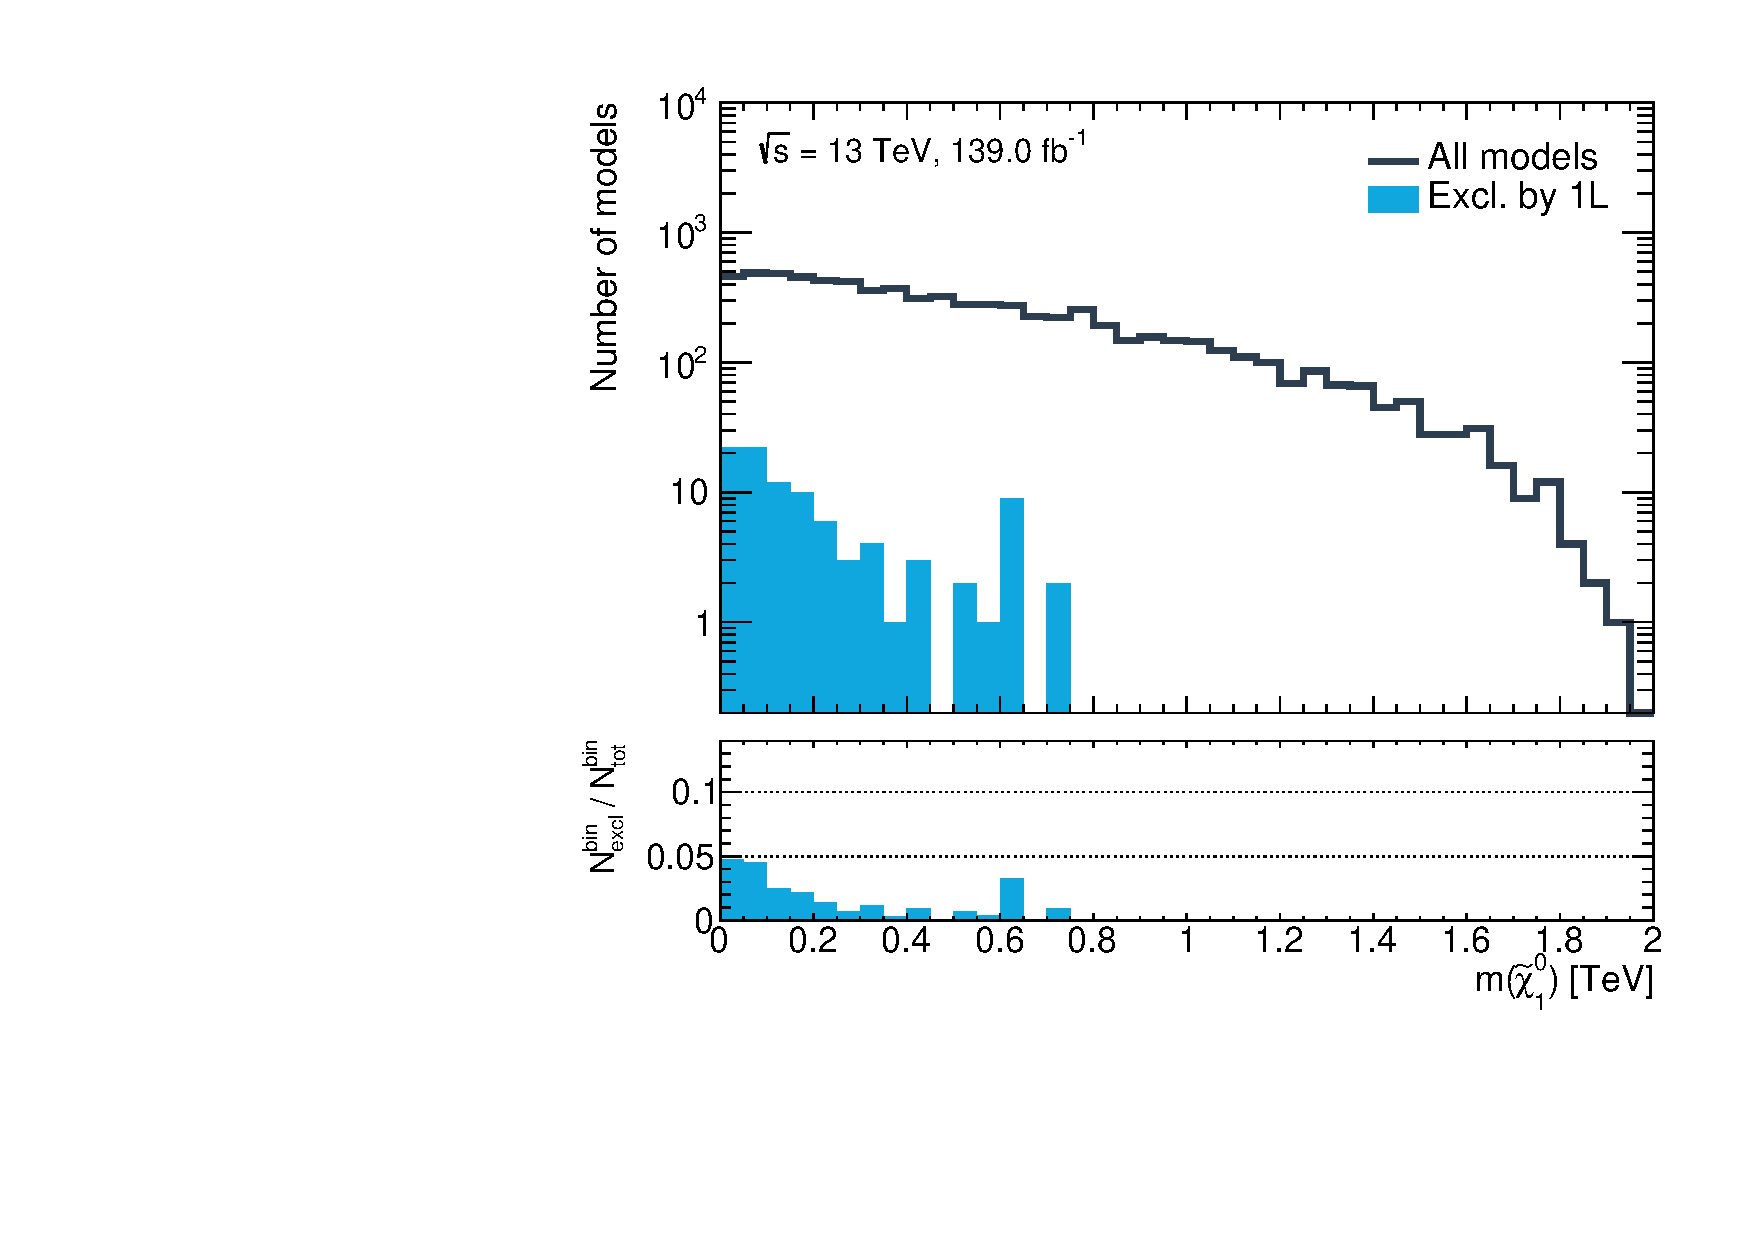
\includegraphics[width=\textwidth]{1D/m_chi_10}
	\end{subfigure}\hfill
	\begin{subfigure}[b]{0.5\linewidth}
		\centering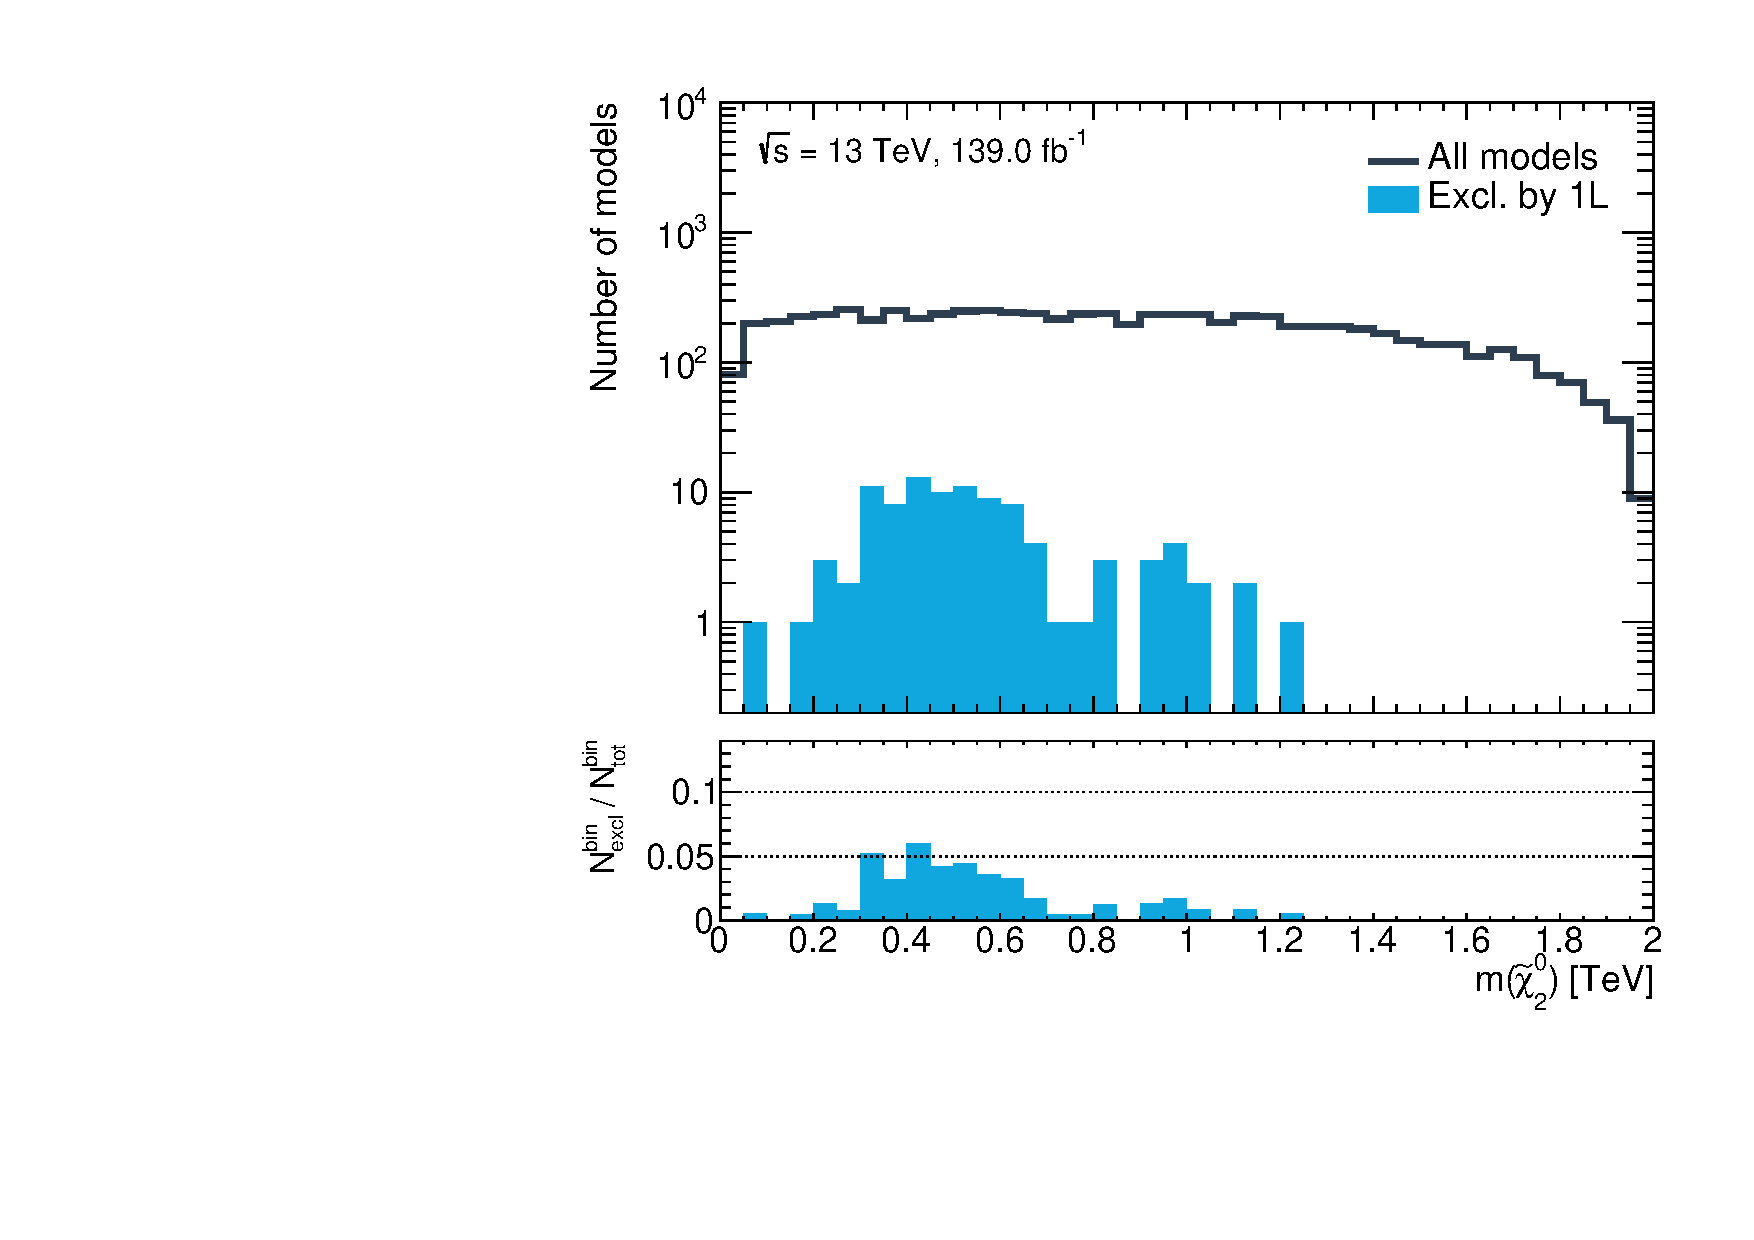
\includegraphics[width=\textwidth]{1D/m_chi_20}
	\end{subfigure}\hfill
	\begin{subfigure}[b]{0.5\linewidth}
		\centering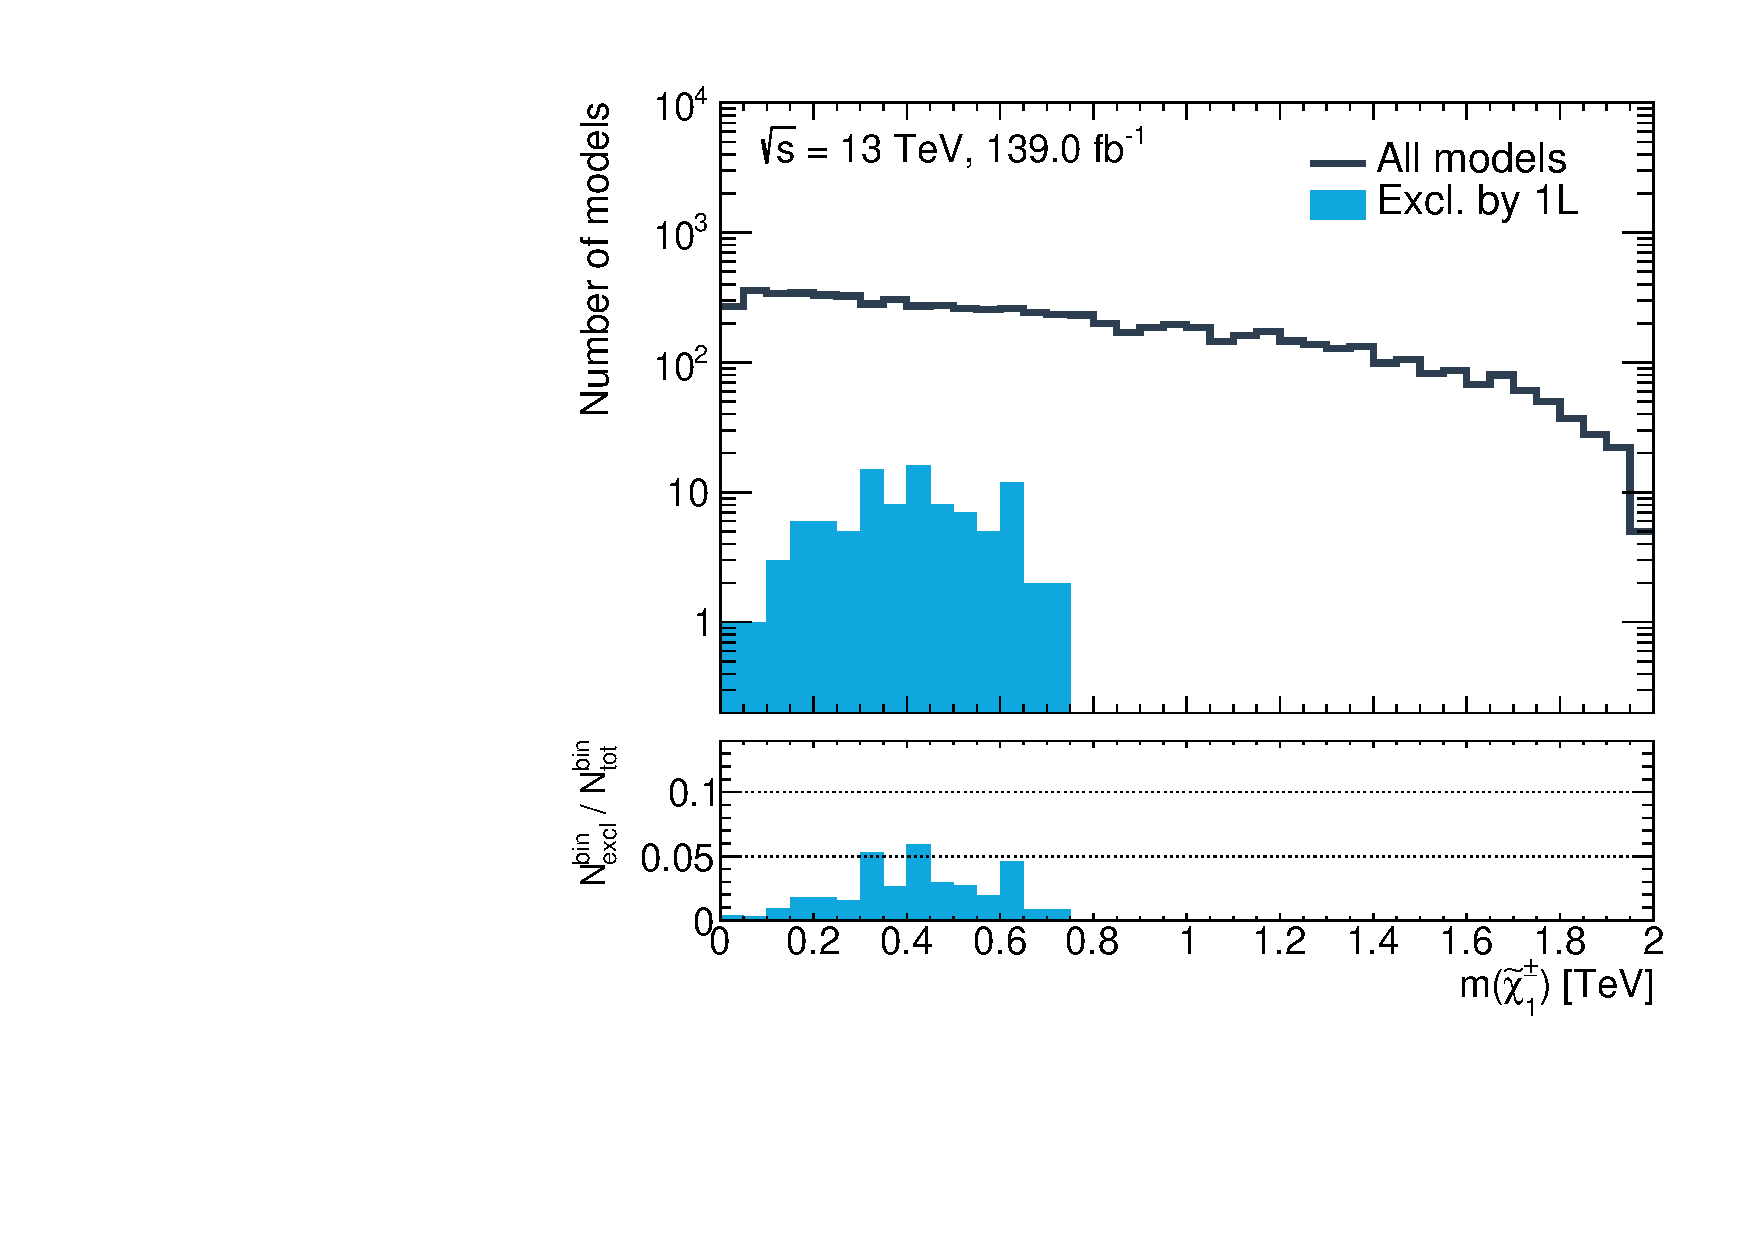
\includegraphics[width=\textwidth]{1D/m_chi_1p}
	\end{subfigure}\hfill
	\caption{}
	\label{fig:impact_electroweakinos_1D}
\end{figure}


\Cref{fig:impact_electroweakinos_2D,fig:impact_electroweakinos_1D} show the bin-by-bin fractions of models excluded by the \onelepton search as two- and one-dimensional distributions, respectively. From the $\charg$--$\lsp$ plane in \cref{fig:mchi1p_mlsp_contour}, it can be seen that the \onelepton search is most sensitive to \gls{pmssm} models in mass ranges similar to those excluded in the context of the simplified model. Most of the models excluded have $\charg$/$\neutr$ masses ranging from roughly $\SI{200}{\GeV}$ to about $\SI{700}{\GeV}$ and \gls{lsp} ranging masses from $\SI{0}{\GeV}$ to about $\SI{300}{\GeV}$. The proportion of excluded models peaks at $m(\charg,\neutr) \approx \SI{450}{\GeV}$ and light \glspl{lsp} with $\lsp < \SI{150}{\GeV}$, as visible in~\cref{fig:impact_electroweakinos_1D}. 

The models excluded by the \onelepton search can roughly be classified in two categories: models lying within the simplified model exclusion contour and models with nearly mass-degenerate $\charg$ and $\neutr$. As discussed in \cref{sec:lsp_pheno}, most models within the simplified model exclusion contour produce a bino-like \gls{lsp} and result in nearly mass-degenerate $\charg$ and $\neutr$. \Cref{fig:impact_electroweakinos_2D_bino_lsp} illustrates this behaviour further. Expectedly, the \onelepton search is thus most sensitive to $\charg\neutr$ production with wino-like electroweakinos and a bino-like $\lsp$, corresponding to models with a spectrum close to that of the canonical simplified model signature originally considered in the search. 

The second category of models excluded comprises cases where the \gls{lsp} is wino-like and nearly mass-degenerate with the $\charg$, corresponding to the diagonal in~\cref{fig:mchi1p_mlsp_contour} As the mass difference between the \gls{lsp} and the $\charg$ is typically much smaller than the \textit{W} boson mass, the $\charg$-decay  primarily proceeds through off-shell \textit{W} bosons, $\charg \rightarrow W^* \lsp$, resulting in soft leptons that often cannot be reconstructed in the analysis. Even though no sensitivity to these models is expected from the \onelepton search, a small set of models with a wino-like \gls{lsp} can still be excluded. These correspond to cases where the $\tilde{\chi}^\pm_2$ is not too heavy such that the \onelepton search is sensitive to $\tilde{\chi}^\pm_2\neutr$ production with cross sections of $\mathcal{O}(\SI{1}{\femto\barn})$. If the $\tilde{\chi}^\pm_2$ decays directly into the \gls{lsp} via $\tilde{\chi}^\pm_2 \rightarrow W^\pm \lsp$, enough events with an isolated lepton can occur, allowing to exclude the model. (see \eg~\cref{fig:mchi10_mchi2p_contour_wino_lsp}).

No sensitivity is observed for \gls{pmssm} models with higgsino-like electroweakinos and thus compressed mass spectra. This is expected, as such scenarios typically produce off-shell \textit{W}, \textit{Z} and \textit{h} bosons, resulting in very soft final state objects the \onelepton search is not optimised for. Dedicated searches (see \eg \reference\cite{SUSY-2018-16}) exist in ATLAS to target such compressed scenarios and work is ongoing to include these in the scans of the \gls{pmssm}.

 \begin{figure}
	\centering
	\begin{subfigure}[b]{0.5\linewidth}
		\centering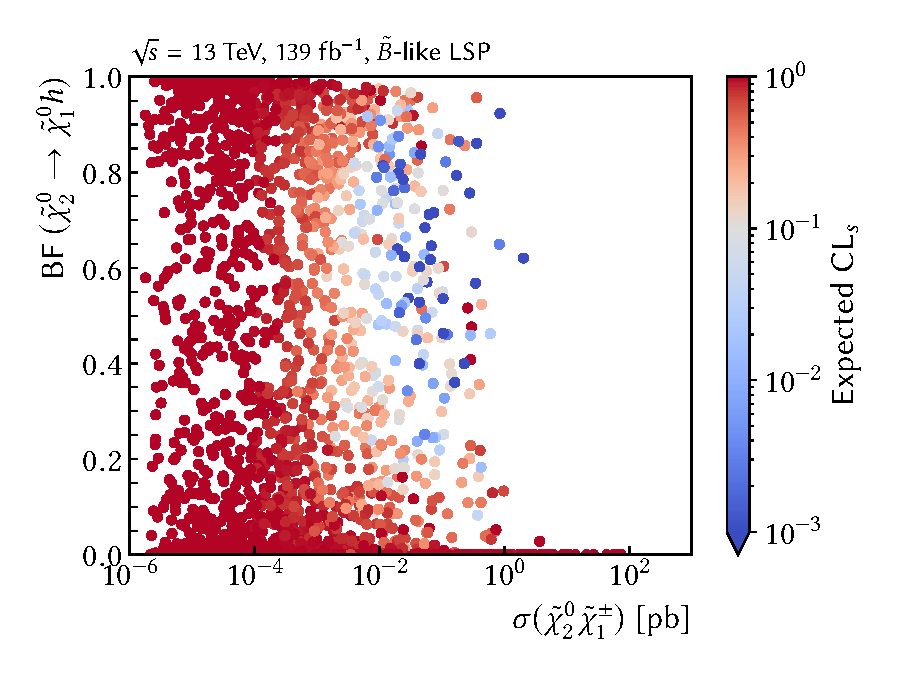
\includegraphics[width=\textwidth]{scatter/fig_scatter_xsec_BFHiggs_bino}
		\caption{\label{fig:fig_scatter_xsec_BFHiggs_bino}}
	\end{subfigure}\hfill
	\begin{subfigure}[b]{0.5\linewidth}
		\centering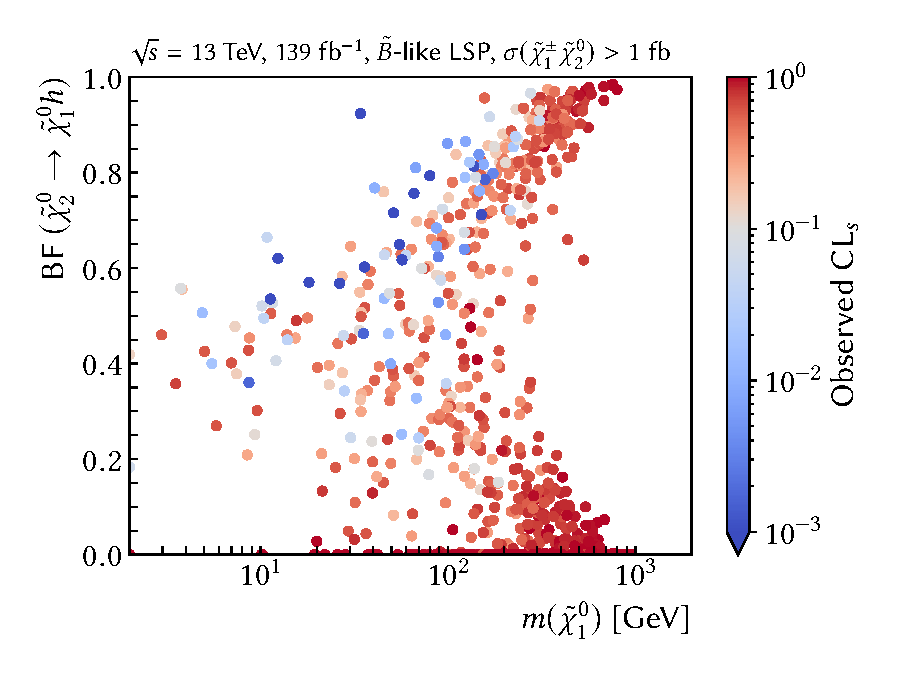
\includegraphics[width=\textwidth]{scatter/fig_scatter_mchi10_BFHiggs_bino_withXsecCut}
		\caption{\label{fig:fig_scatter_mchi10_BFHiggs_bino_withXsecCut}}
	\end{subfigure}\hfill
	\caption{}
	\label{fig:bino_sensitivity}
\end{figure}

In general, the sensitivity to \gls{pmssm} models is significantly reduced compared to the simplified model exclusion contour, even in the parameter space generating models similar to the simplified model. The crucial difference, responsible for the loss in sensitivity, is the fact that the simplified model assumes branching ratios of 100\% of the $\charg \rightarrow W^\pm \lsp$ and $\neutr \rightarrow h \lsp$ decays. While the former is in general a good assumption in \gls{pmssm} models where $m(\charg)\lesssim m(\neutr)$, the latter often is not the dominant decay of the $\neutr$ which may decay through $\neutr \rightarrow Z \lsp$ instead. The couplings of the $\neutr$ to the Higgs boson are suppressed by powers of $\vert\mu\vert/M_2$ in the gaugino-like regions~\cite{Arbey:2012fa}, meaning that the branching fraction of $\neutr \rightarrow h \lsp$ takes on reasonably high values only in models with an \gls{lsp} containing a substantial bino component. The Higgs coupling suppression is illustrated in \cref{fig:higgs_coupling_neutralino}. As can be seen from~\cref{fig:mchi1p_mlsp_contour}, even in the bulk of the $\charg$--$\lsp$ plane---containing mostly models with a bino-like \gls{lsp}---not all models can be excluded by the \onelepton search. \Cref{fig:fig_scatter_xsec_BFHiggs_bino} shows that many of these models have either a too small $\charg\neutr$ pair-production cross section or too low values for $\mathrm{BF}(\neutr \rightarrow h \lsp)$. For the few non-excluded models with reasonable $\charg\neutr$ pair-production cross section ($> \mathcal{O}(\SI{1}{\femto\barn})$) and high enough Higgs coupling to $\neutr$, the mass of the \gls{lsp} turns out to be too high (see \cref{fig:fig_scatter_mchi10_BFHiggs_bino_withXsecCut}), typically resulting in final states with insufficient $\etmiss$ and soft objects.  

As a cross-check, a significant portion of the models with bino-like \gls{lsp} were reprocessed with $\mathrm{BF}(\neutr \rightarrow h \lsp)$ fixed to unity and subsequently analysed with the \onelepton search. The results can be seen in \Cref{fig:mchi1p_mchi20_contour_bino_lsp_wh_only}, revealing that significantly more models can be excluded within the simplified model contour when the simplified model branching fraction assumption is restored. As the $\neutr$ decay into a $Z$ boson and $\lsp$ is the competing decay to $\neutr \rightarrow h \lsp$, combining searches targeting these decay modes could recover the loss in sensitivity. Likewise, the development of searches targeting both decay modes at the same time would also recover the full sensitivity\footnote{Provided that they are targeted with disjoint signal regions such that a combined likelihood can be built.}.  

\subsection{Impact on pMSSM parameters}


 \begin{figure}
	\centering
	\begin{subfigure}[b]{0.5\linewidth}
		\centering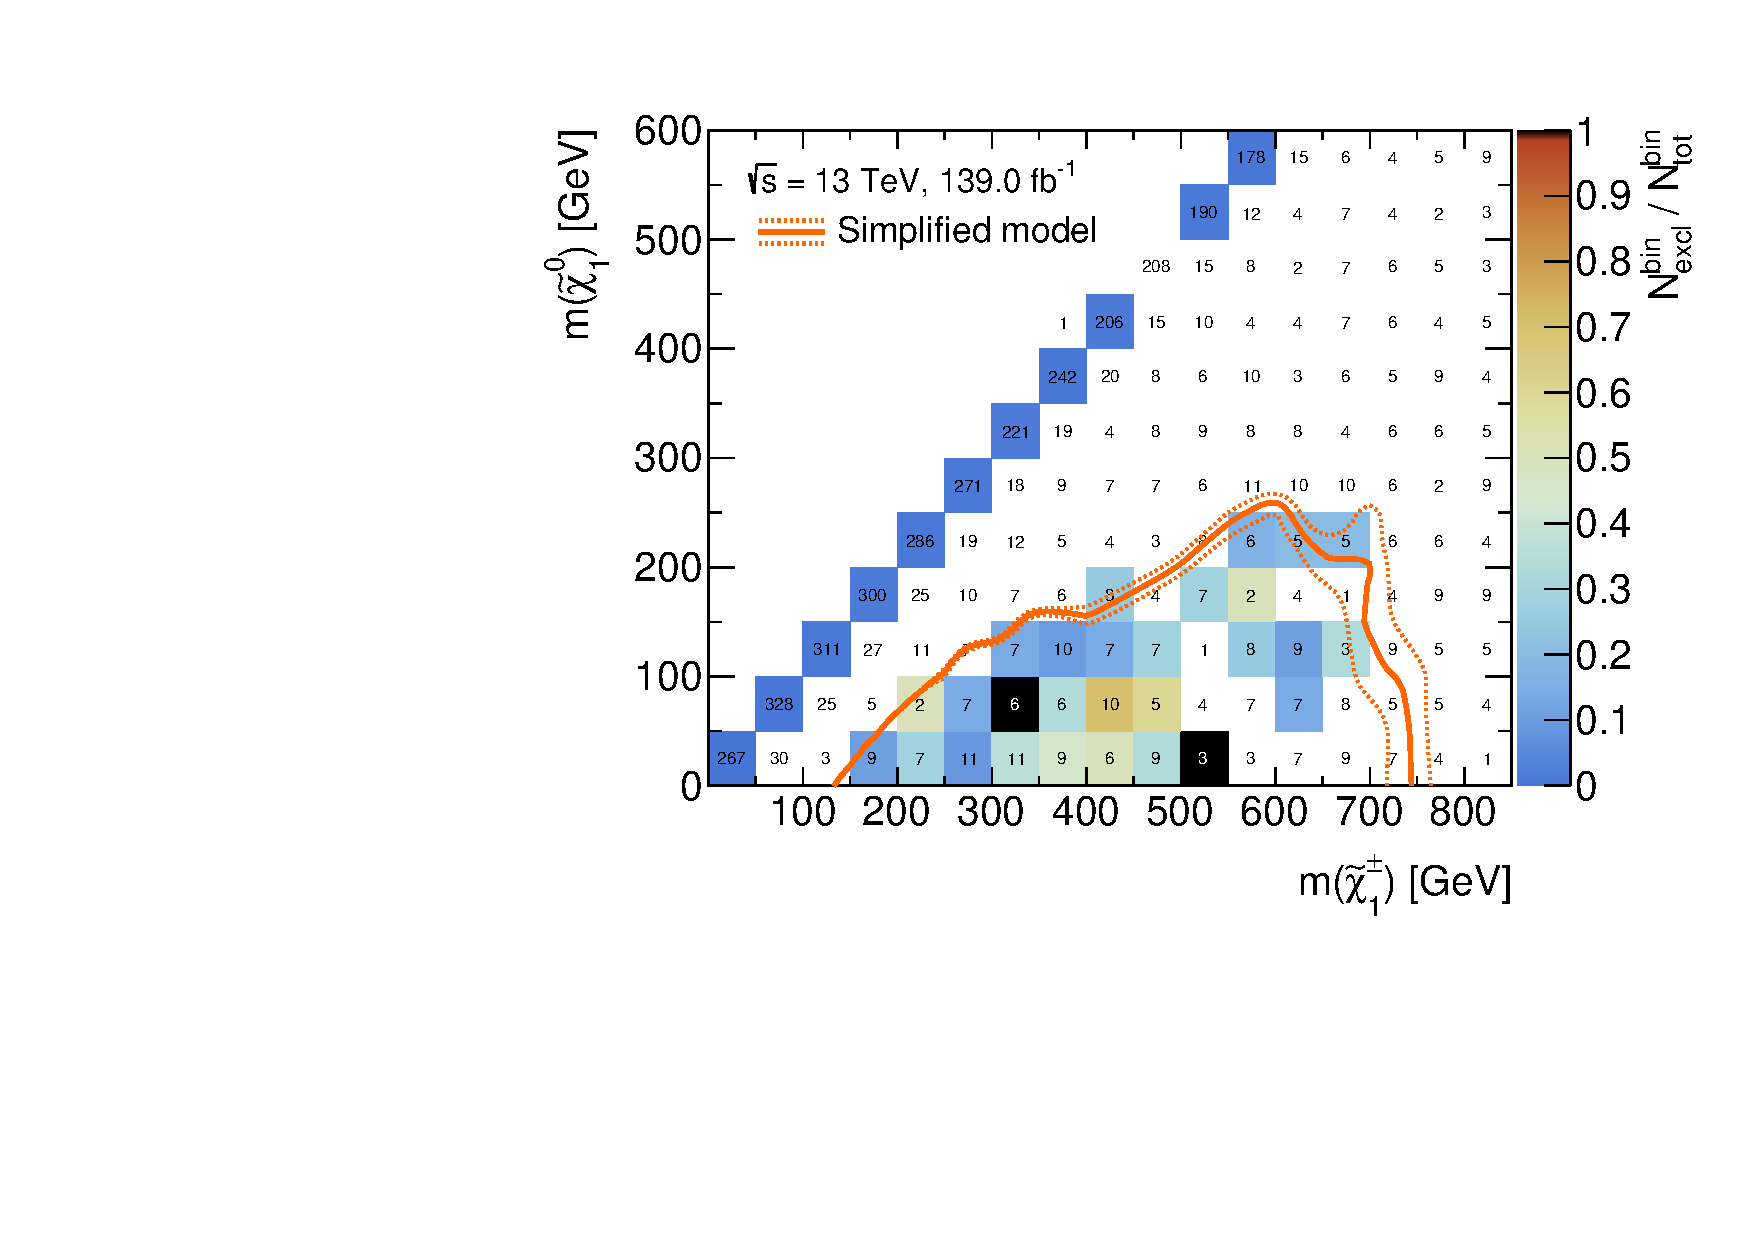
\includegraphics[width=\textwidth]{cut_none/mchi1p_mlsp_contour}
		\caption{\label{fig:mchi1p_mlsp_contour}}
	\end{subfigure}\hfill
	\begin{subfigure}[b]{0.5\linewidth}
		\centering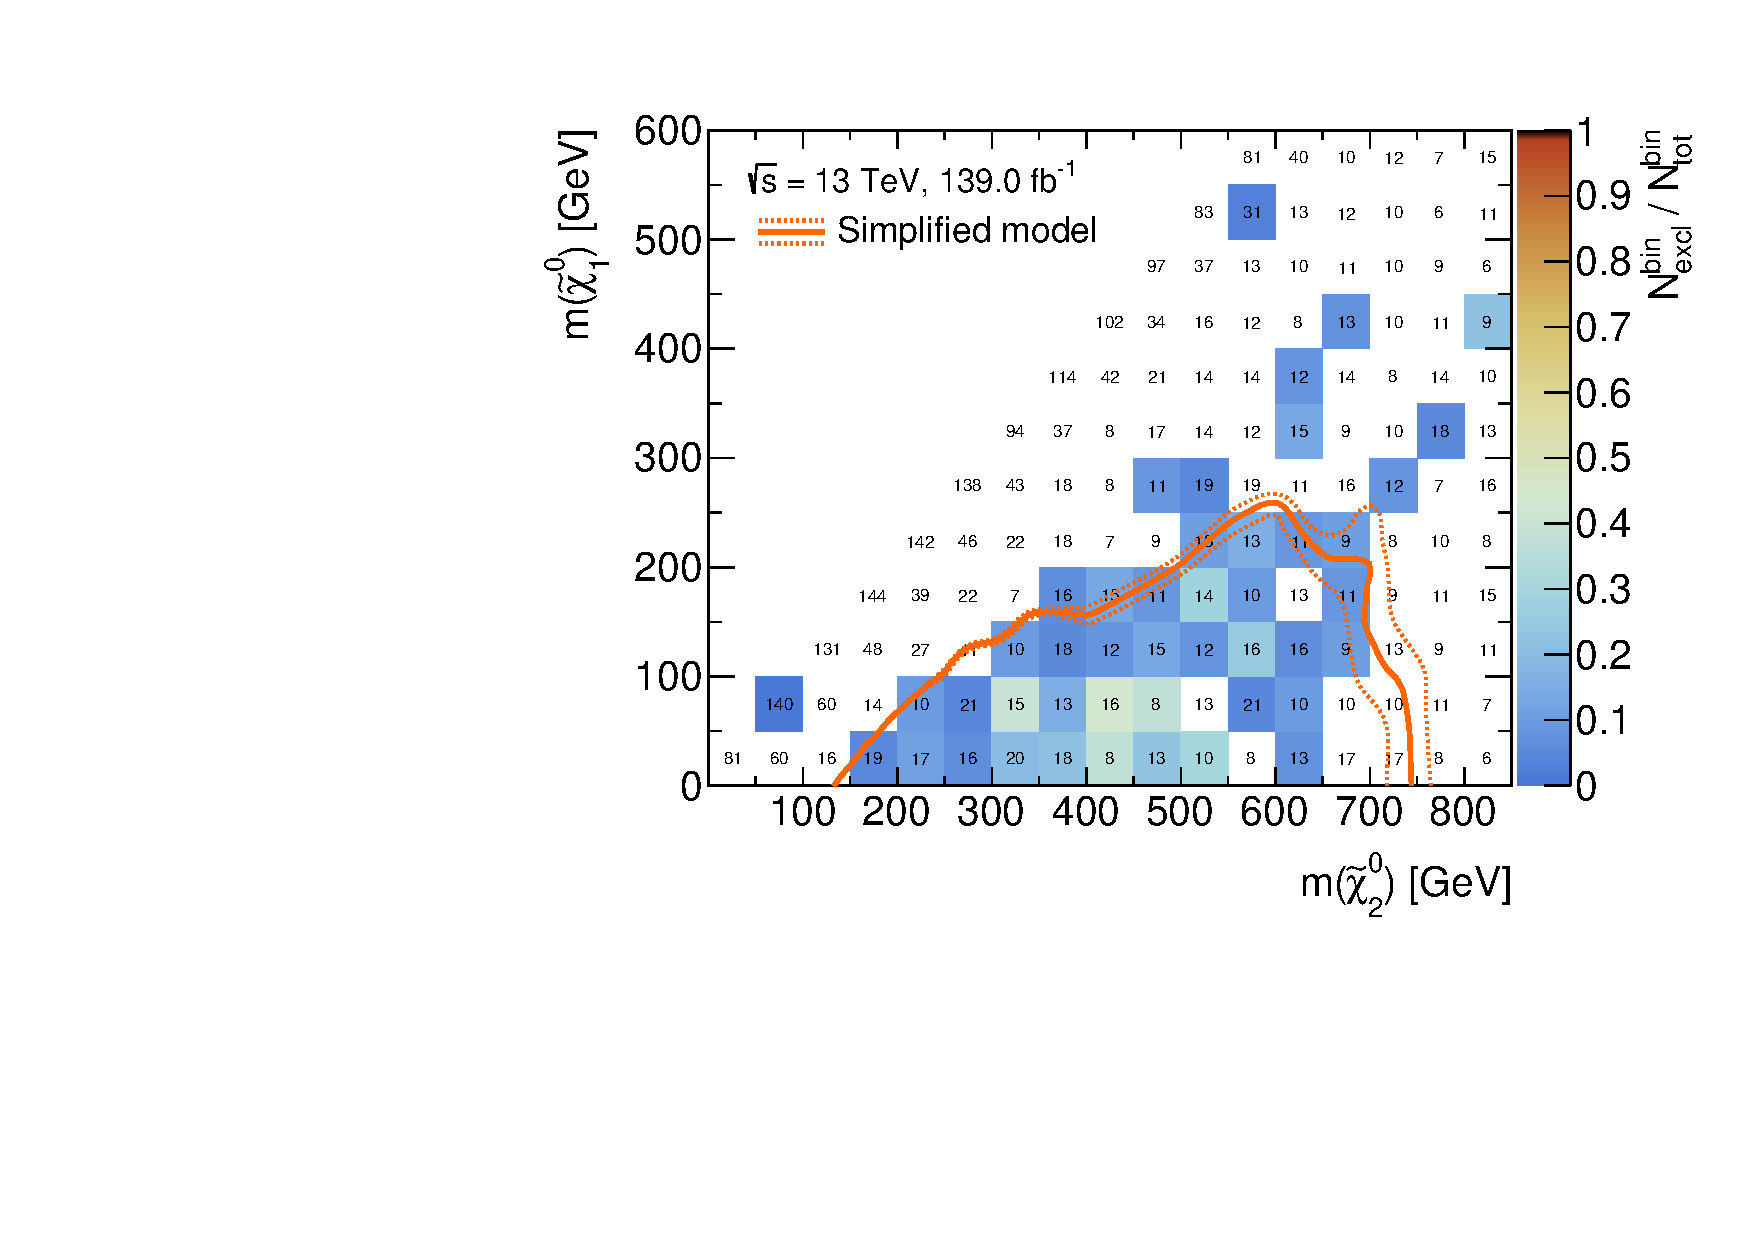
\includegraphics[width=\textwidth]{cut_none/mchi20_mlsp_contour}
		\caption{\label{fig:mchi20_mlsp_contour}}
	\end{subfigure}\hfill
	\begin{subfigure}[b]{0.5\linewidth}
		\centering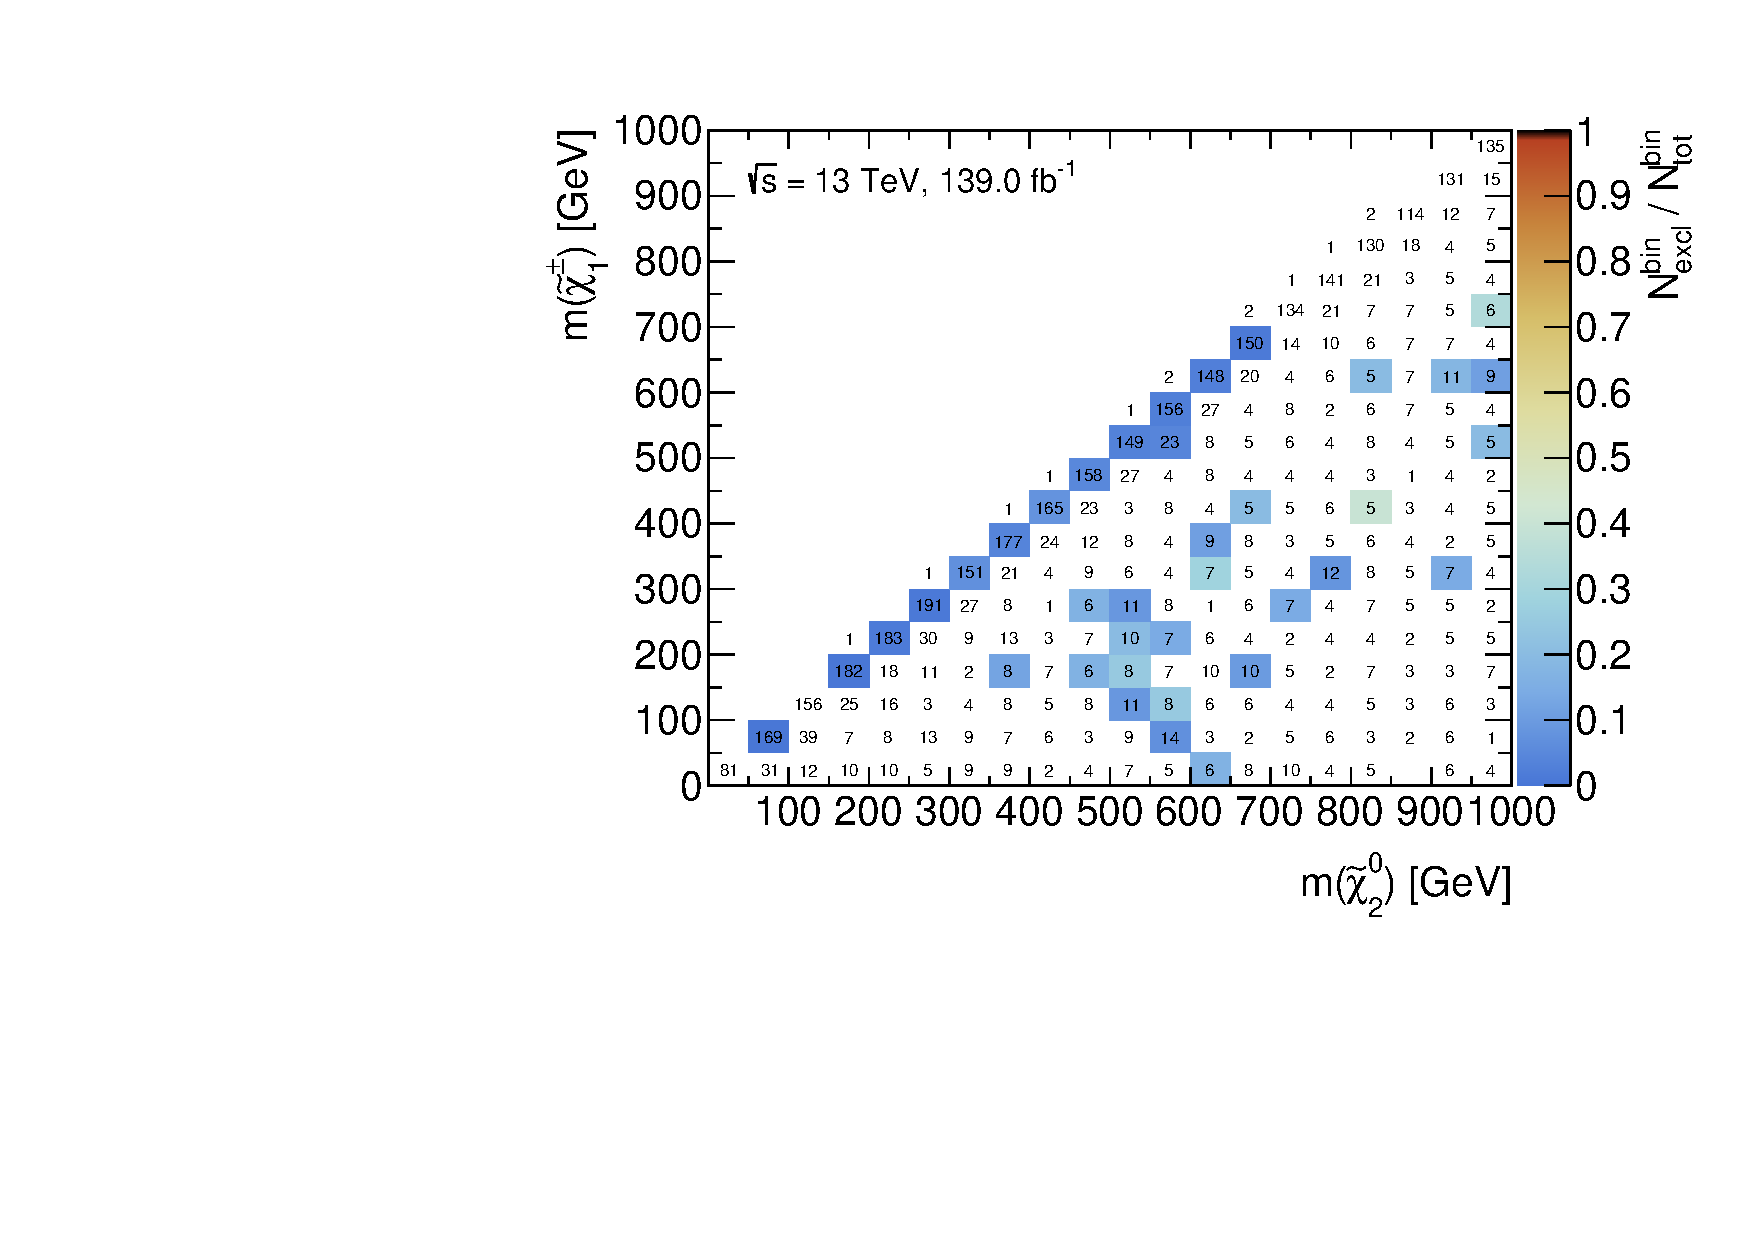
\includegraphics[width=\textwidth]{cut_none/mchi1p_mchi20_contour}
		\caption{\label{fig:mchi1p_mchi20_contour}}
	\end{subfigure}\hfill
	\caption{Bin-by-bin fraction of excluded models as a function of the relevant sparticle masses. The numbers in the bins correspond to the total number of models sampled falling into the respective bin. The number of models excluded by the 1-lepton analysis is encoded with a colour bar ranging from 0 to 1. Where all models in a given bin are excluded, the bin is coloured in black. Bins without any models excluded are left white. Models are evaluated using the simplified likelihood of the 1-lepton analysis. The simplified model contour is shown in orange.}
	\label{fig:impact_electroweakinos_2D}
\end{figure}


 \begin{figure}
	\centering
	\begin{subfigure}[b]{0.5\linewidth}
		\centering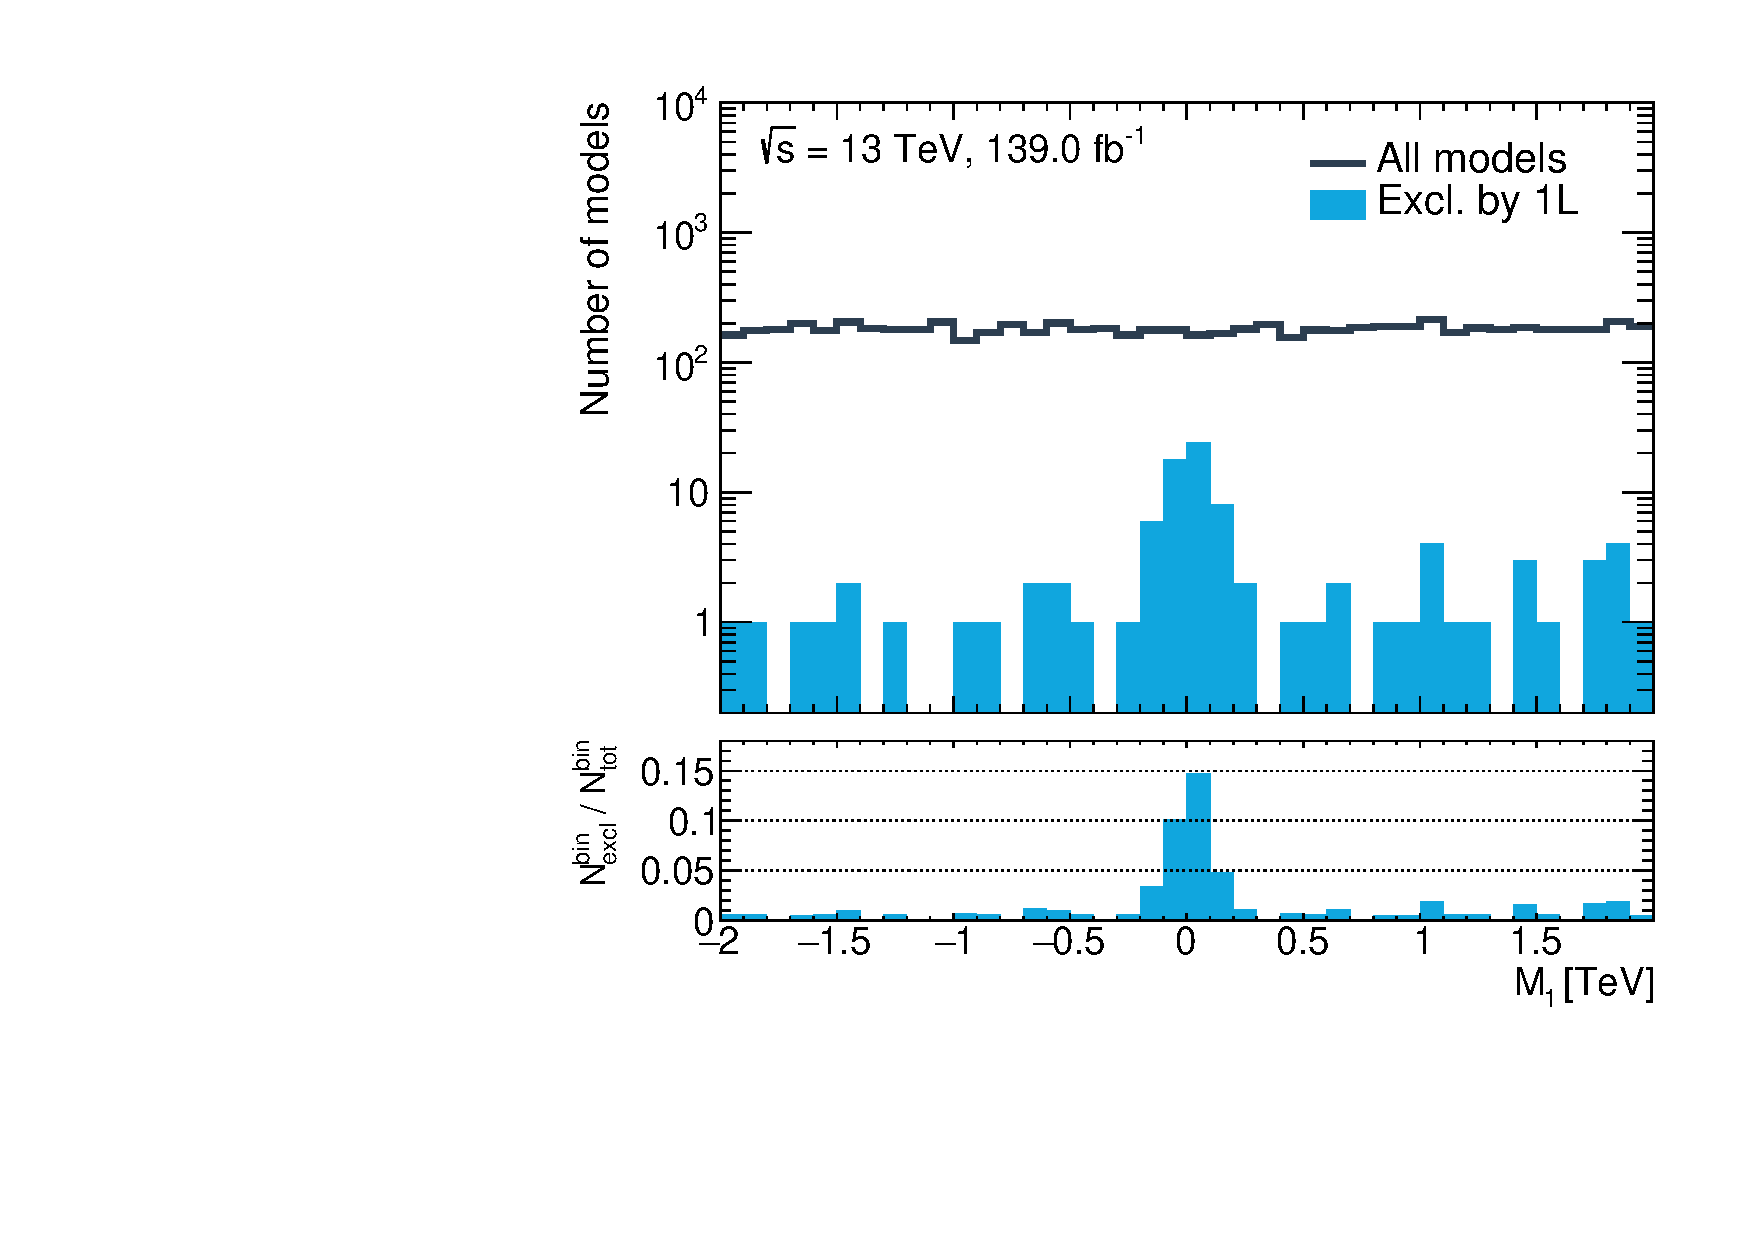
\includegraphics[width=\textwidth]{1D/M1}
	\end{subfigure}\hfill
	\begin{subfigure}[b]{0.5\linewidth}
		\centering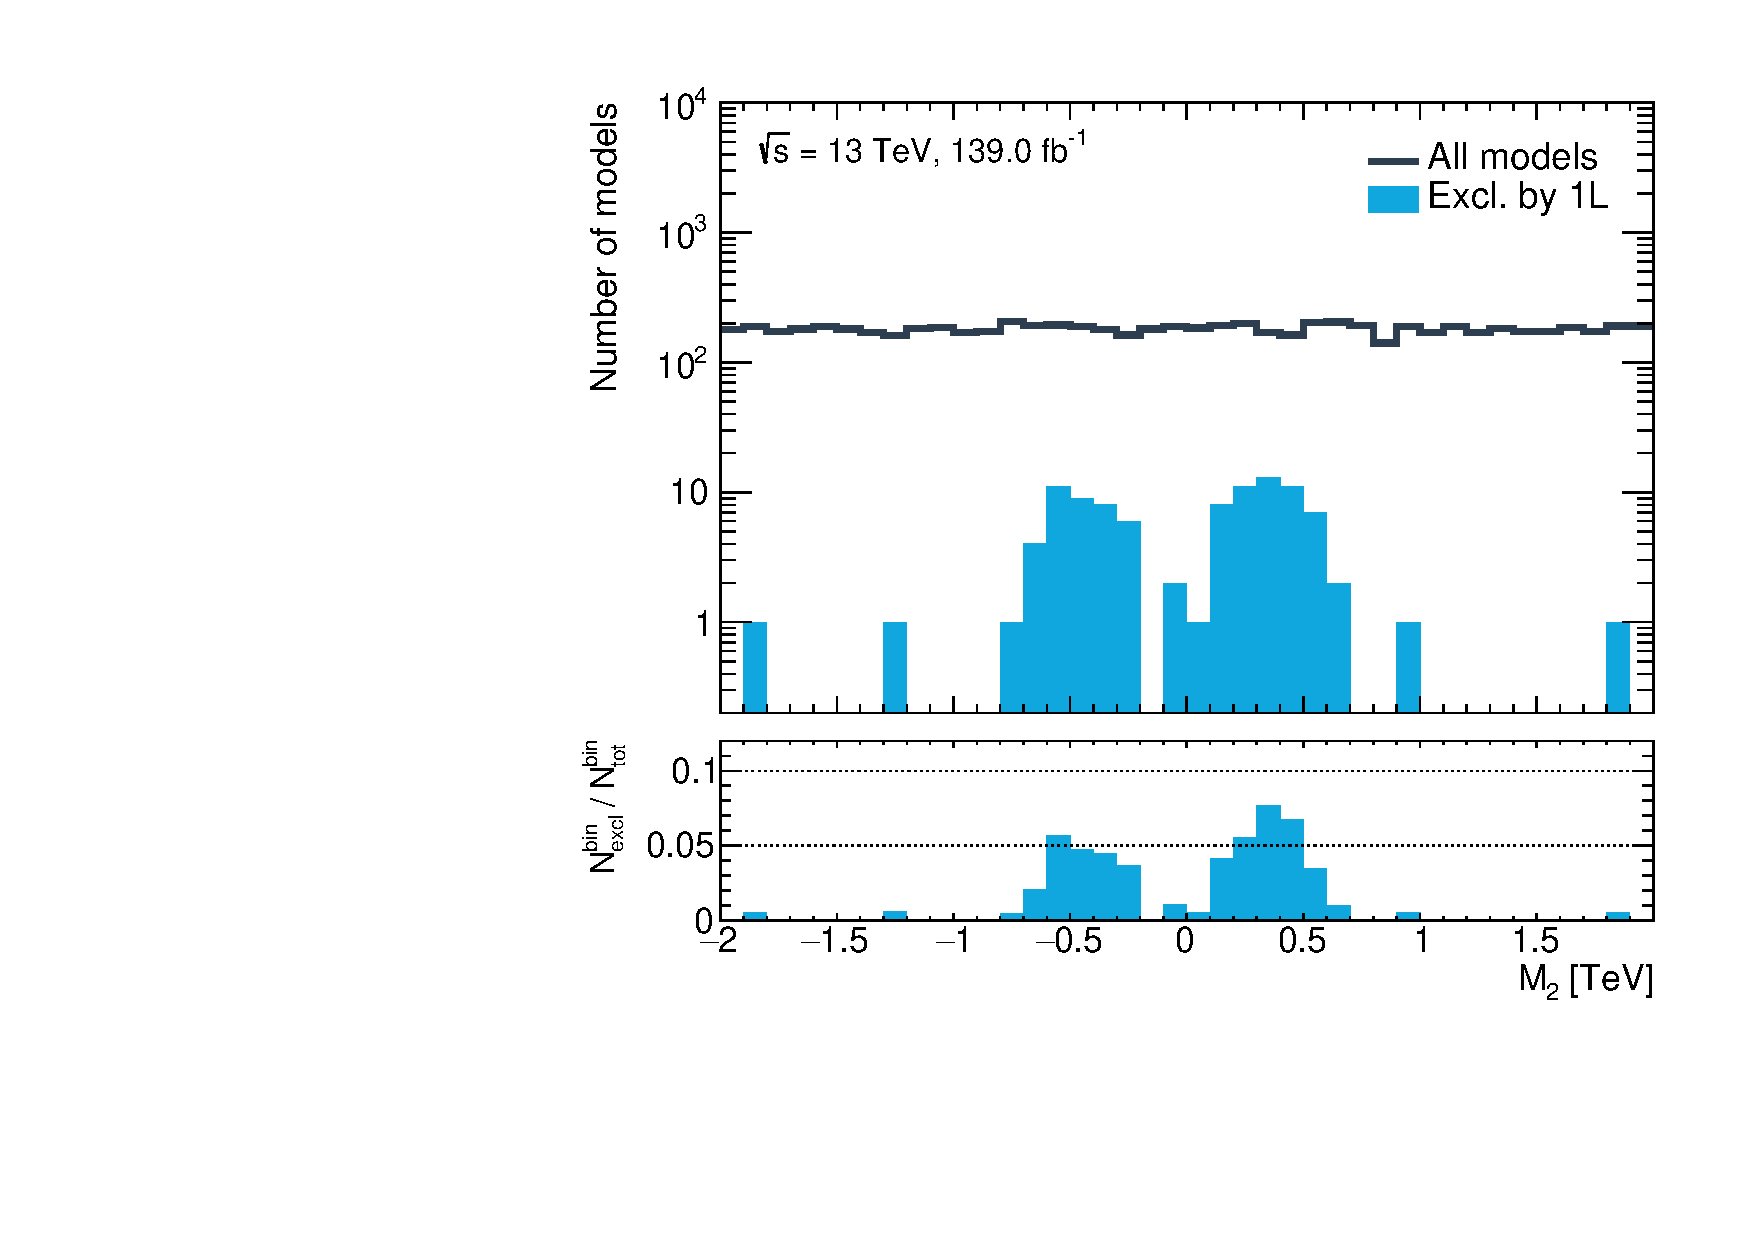
\includegraphics[width=\textwidth]{1D/M2}
	\end{subfigure}\hfill
	\begin{subfigure}[b]{0.5\linewidth}
		\centering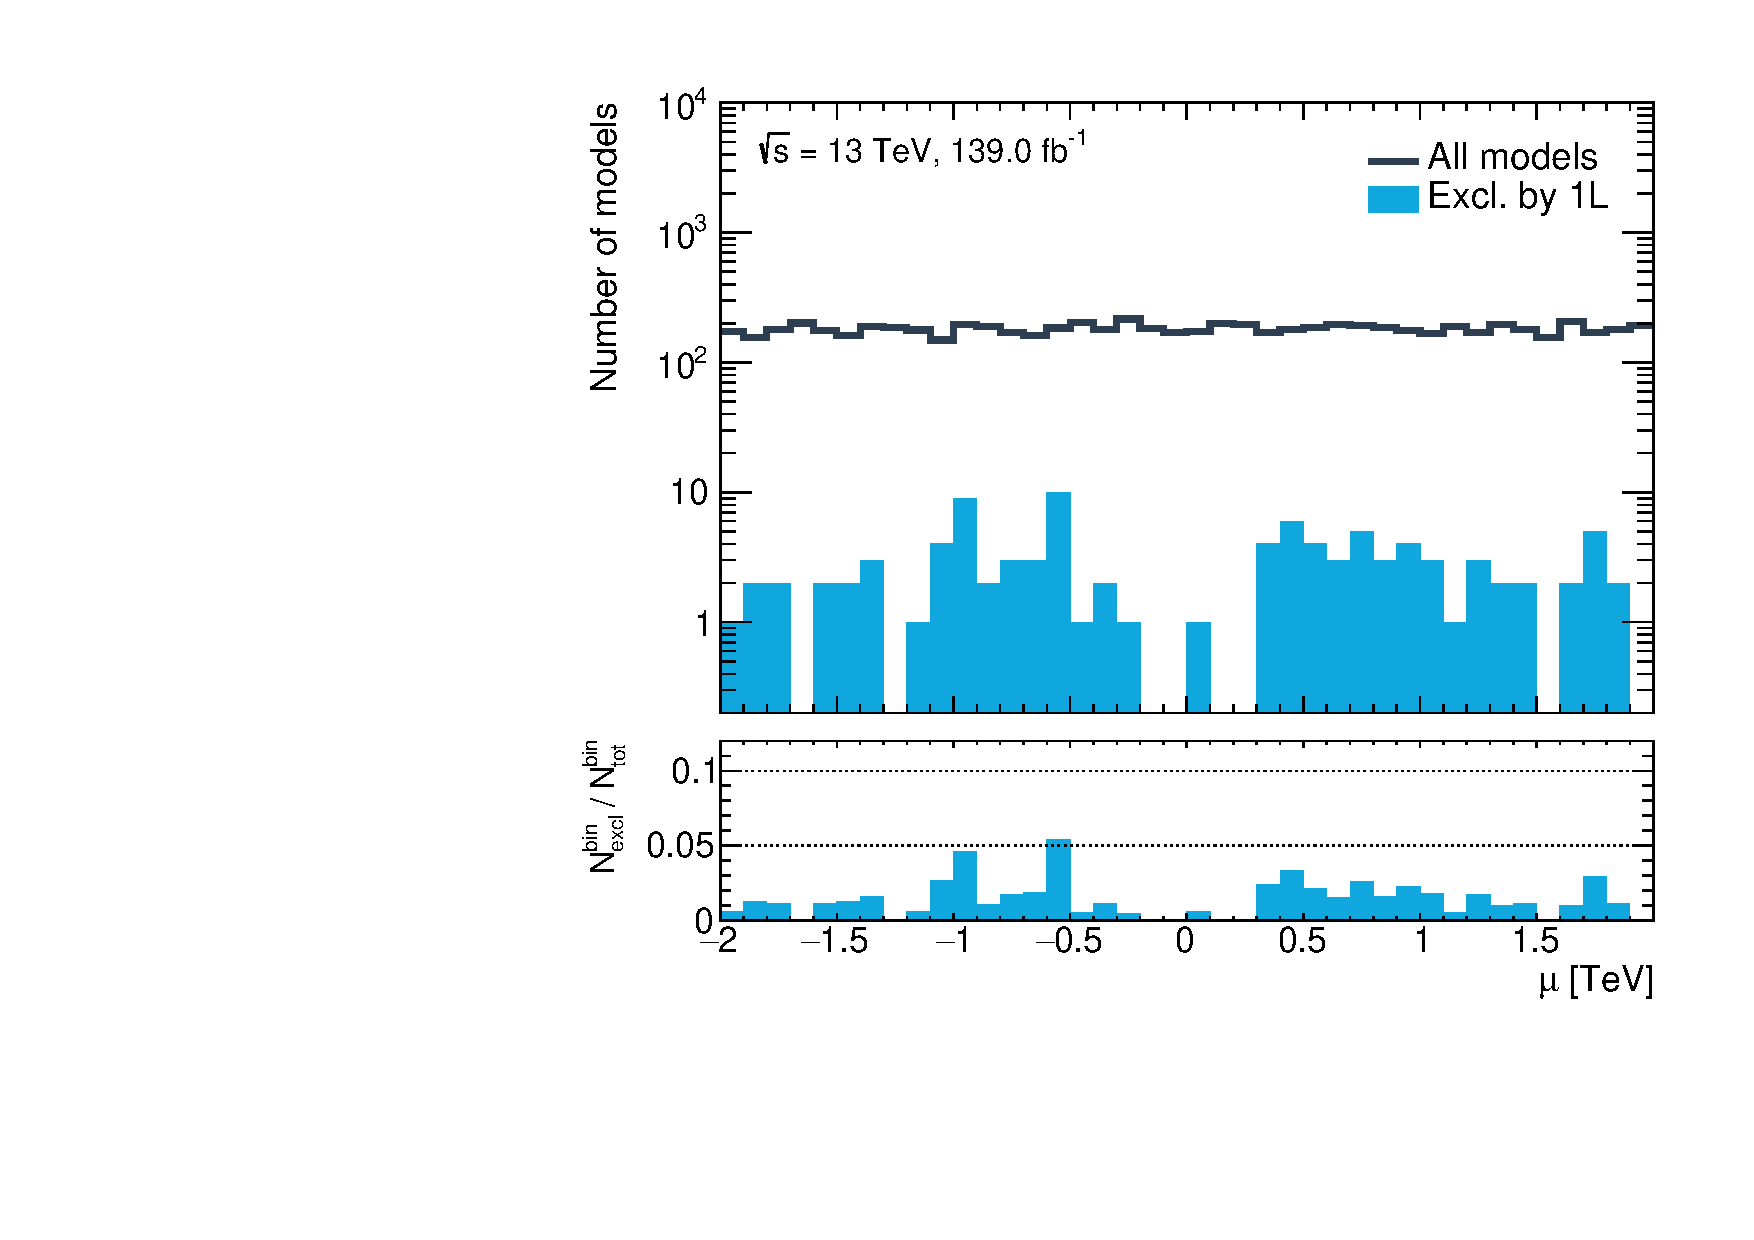
\includegraphics[width=\textwidth]{1D/mu}
	\end{subfigure}\hfill
	\begin{subfigure}[b]{0.5\linewidth}
		\centering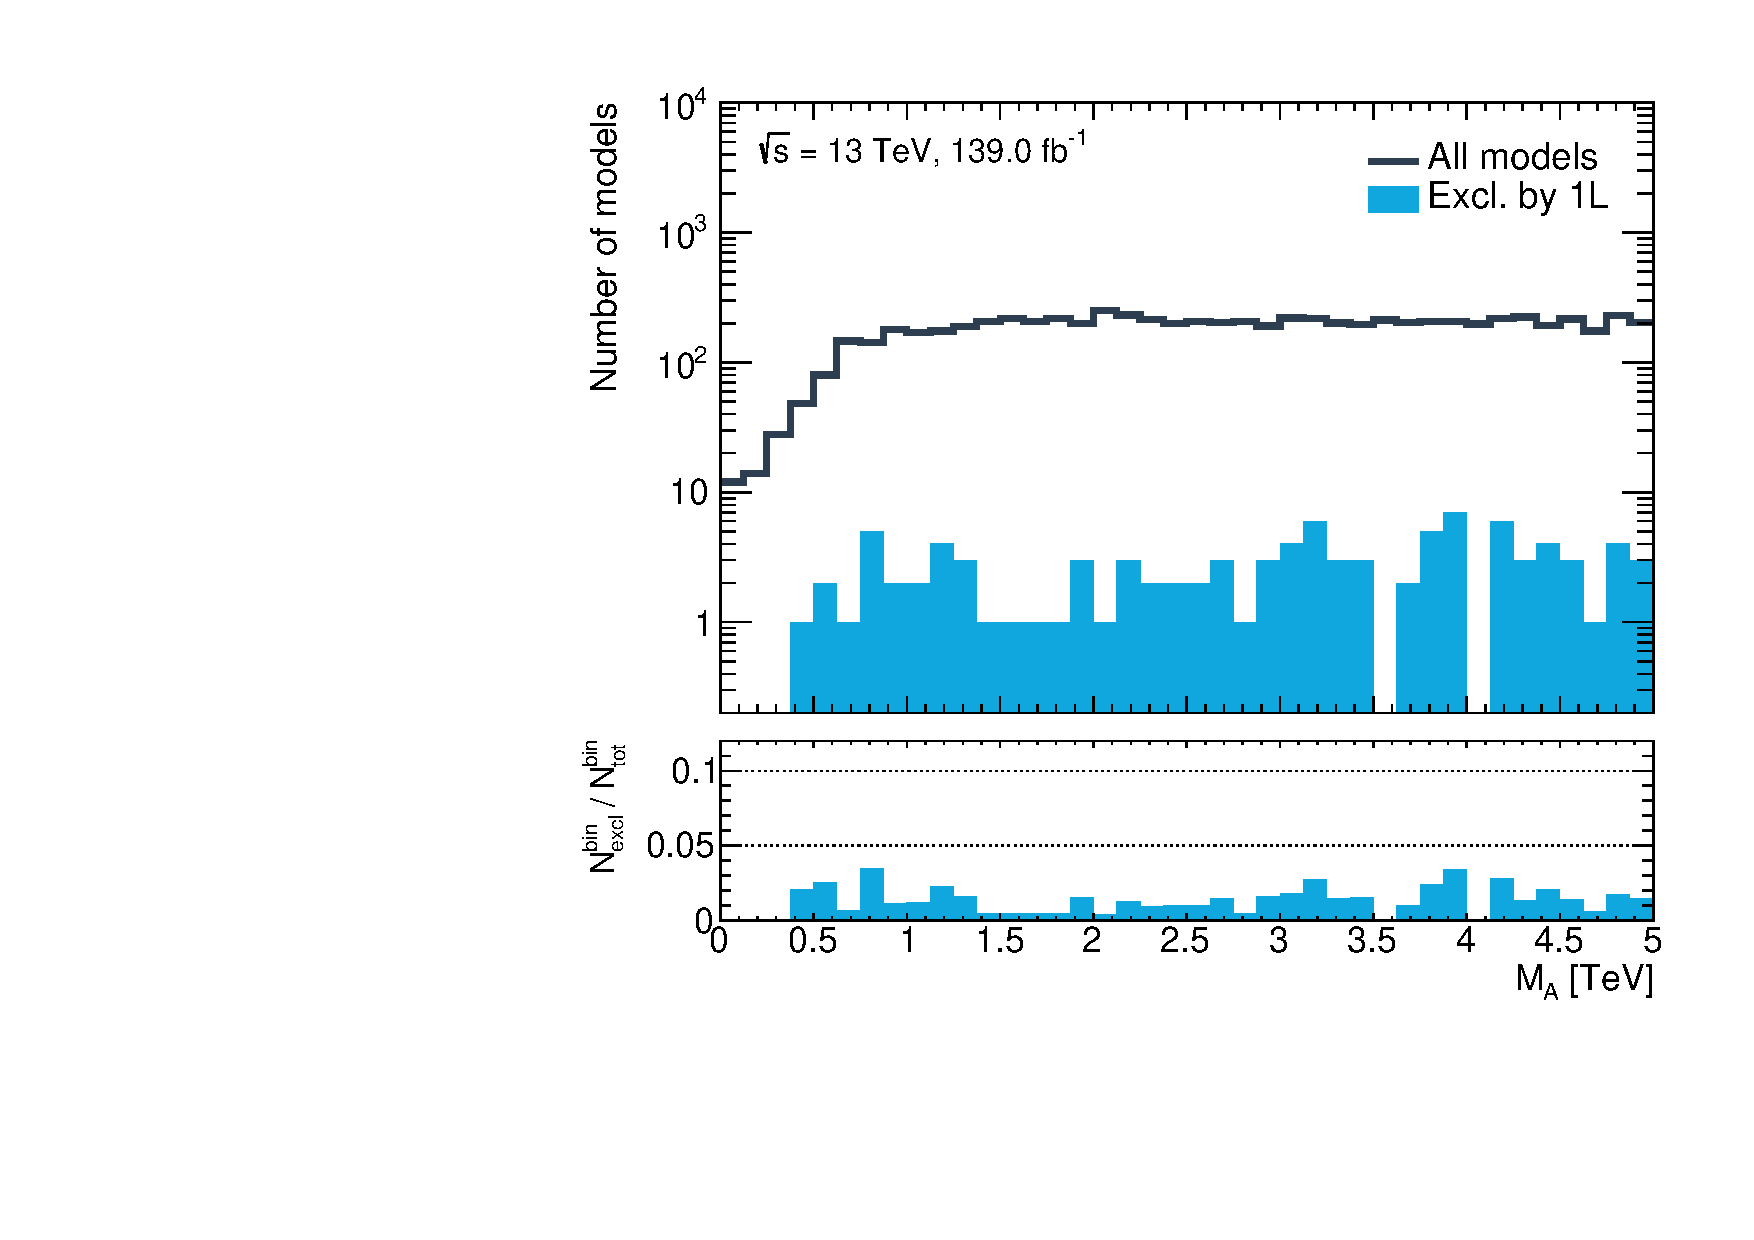
\includegraphics[width=\textwidth]{1D/mA}
	\end{subfigure}\hfill
	\begin{subfigure}[b]{0.5\linewidth}
		\centering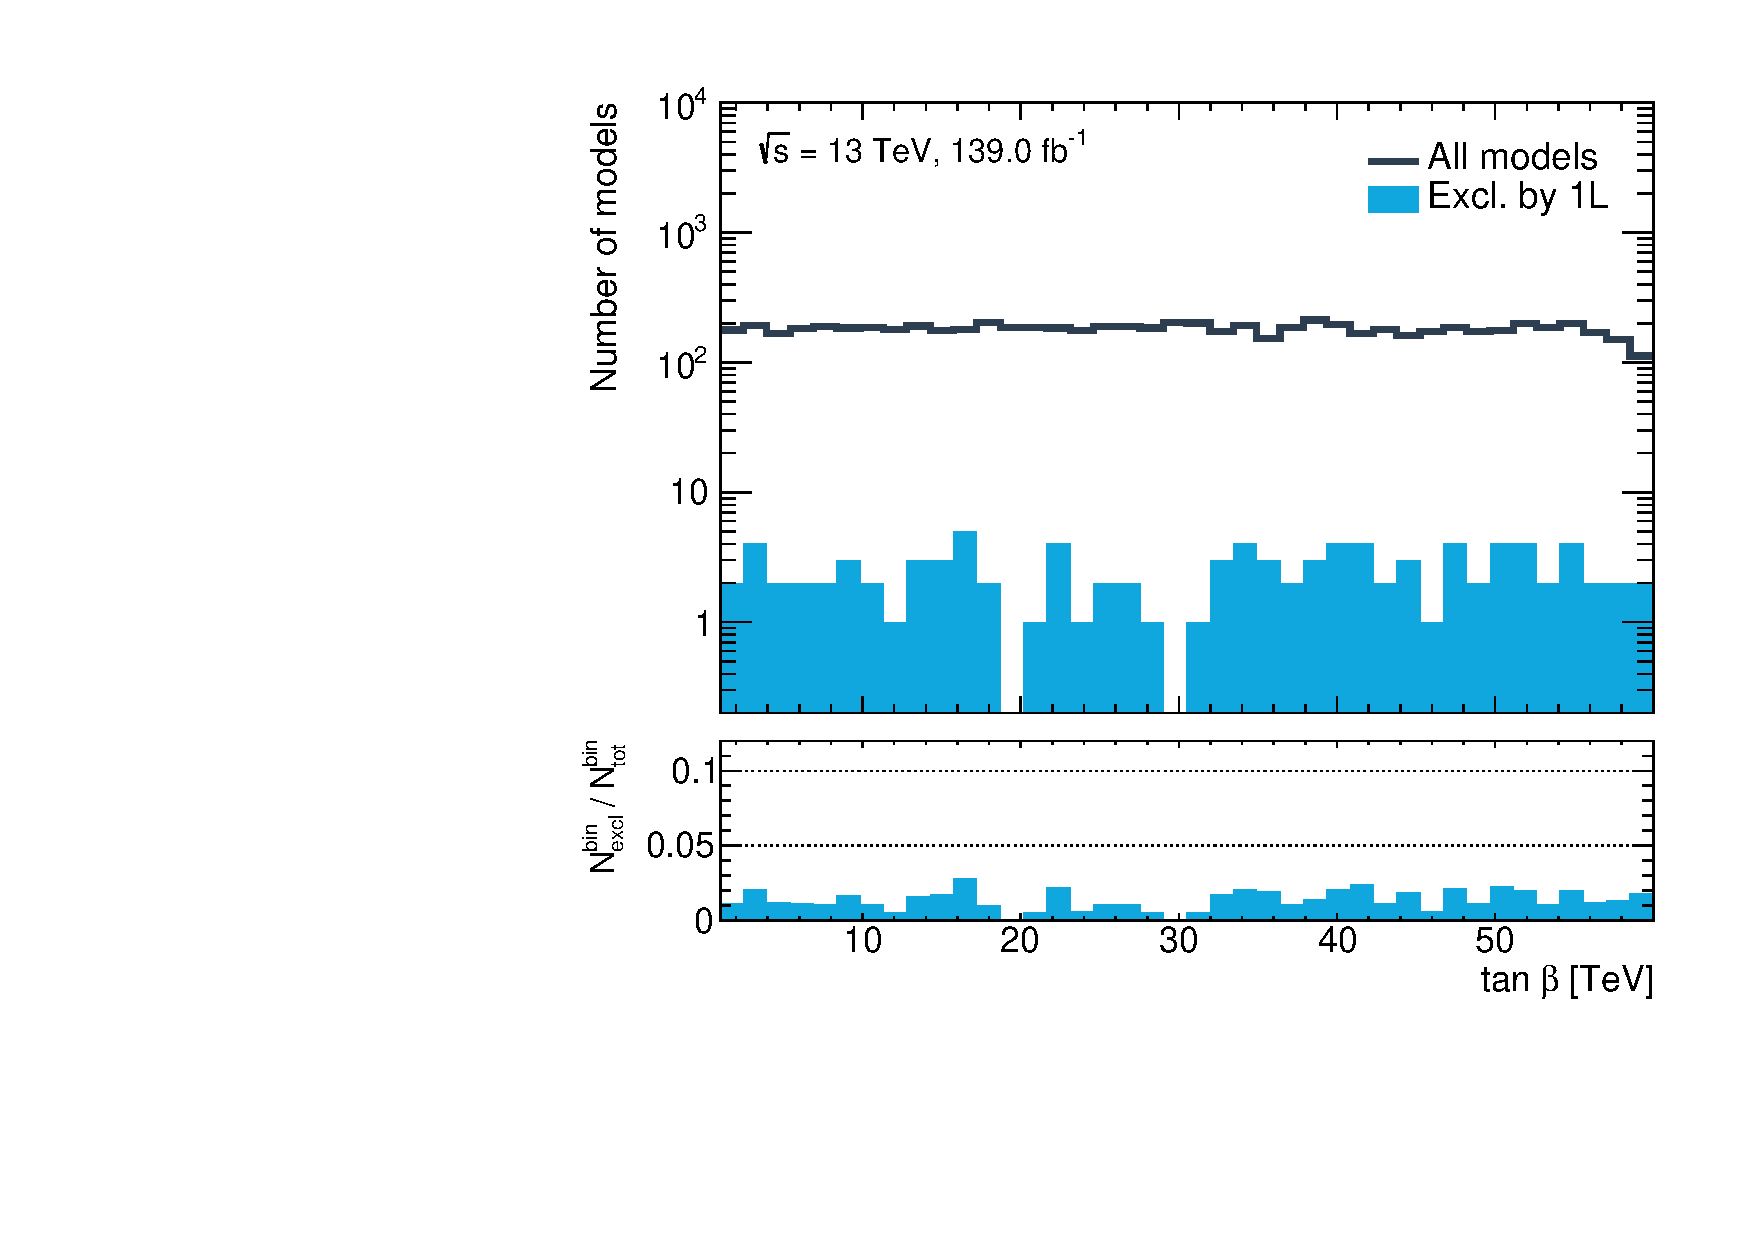
\includegraphics[width=\textwidth]{1D/tanb}
	\end{subfigure}\hfill
	\caption{}
	\label{fig:impact_pMSSM_parameters_1D}
\end{figure}

\subsection{Impact on dark matter}
